% 构建：cd kernels/interview/book/colfax && ./build.sh
% 译自 Colfax Research《Categorical Foundations for CuTe Layouts》
% （arXiv:2601.05972，官方 LaTeX 源 FinalVersion.tex），仅供学习交流。
\documentclass[12pt,a4paper]{ctexrep}
% cf-macros.tex — 移植自 Colfax《Categorical Foundations for CuTe Layouts》官方源
% （arXiv:2601.05972，FinalVersion.tex L1-270 preamble）。
% 改动：①定理环境名中文化 ②xcolor 两次加载合并为一次 ③移除 lmodern/microtype
%（pdflatex 专属，xelatex 下不需要）④增加 longtable（术语表用）。
\usepackage{graphicx}
\usepackage{amsmath}
\usepackage{amsfonts}
\usepackage{amssymb}
\usepackage{amsthm}
\usepackage{tikz-cd}
\usetikzlibrary{matrix,fit,backgrounds}
\usepackage[table,dvipsnames]{xcolor}
\usepackage{mathrsfs}
\usepackage{mathdots}
\usepackage{mathtools}
\usepackage{comment}
\usepackage{array}
\usepackage{algorithm}
\usepackage{algpseudocode}  % breakable algorithmic environment
\usepackage{caption}
\usepackage[most]{tcolorbox}
\usepackage{longtable}
\usepackage{booktabs}

% Algorithm counter (for \ref)
\renewcommand{\thealgorithm}{\arabic{algorithm}}

% Breakable, framed algorithm box with continued title
\newtcolorbox[use counter=algorithm, number within=section]{BreakableAlgorithm}[2][]{%
  enhanced,
  breakable,
  colback=white,
  colframe=black,
  boxrule=0.8pt,
  arc=2pt,
  left=8pt,right=8pt,top=8pt,bottom=8pt,
  attach title to upper,
  title={算法~\thetcbcounter：#2},
  title after break={算法~\thetcbcounter（续）：#2},
  fonttitle=\bfseries,
  colbacktitle=white,
  coltitle=black,
  titlerule=0.8pt,
  borderline north={1pt}{0pt}{black},
  borderline south={1pt}{0pt}{black},
  #1
}

% Subtle line numbers & comment style
\algrenewcommand\alglinenumber[1]{\scriptsize\color{gray}{#1}}
\algrenewcommand{\algorithmiccomment}[1]{\hfill\(\triangleright\)\ #1}

% Horizontal separator you can place inside the algorithm
\newcommand{\algsep}{\Statex \rule{\linewidth}{0.6pt}}
\renewcommand{\baselinestretch}{1.10}
\usepackage[letterpaper,margin=1.2in]{geometry}  % 与原文版心一致（report 默认 letterpaper）
\setlength{\emergencystretch}{3em}  % CJK 行文断行点少，吸收长引用/行内数学小溢出
\usepackage[colorlinks=true, linkcolor=blue, urlcolor=blue, citecolor=blue]{hyperref}
\usepackage{cleveref}
\usepackage{listings}
\usepackage{enumitem}
\usepackage[backend=biber,style=numeric]{biblatex}
\addbibresource{references.bib}

\definecolor{colorx1}{rgb}{1.00, 0.00, 0.00} % Red
\definecolor{colorx2}{rgb}{1.00, 0.75, 0.00} % Orange-yellow
\definecolor{colorx3}{rgb}{0.50, 1.00, 0.00} % Yellow-green
\definecolor{colorx4}{rgb}{0.00, 1.00, 0.50} % Green-cyan
\definecolor{colorx5}{rgb}{0.00, 1.00, 1.00} % Cyan
\definecolor{colorx6}{rgb}{0.00, 0.50, 1.00} % Blue
\definecolor{colorx7}{rgb}{0.50, 0.00, 1.00} % Indigo
\definecolor{colorx8}{rgb}{1.00, 0.00, 1.00} % Magenta

\definecolor{codegray}{rgb}{0.5,0.5,0.5}
\definecolor{codebg}{rgb}{0.95,0.95,0.95}
\lstset{
    backgroundcolor=\color{codebg},
    basicstyle=\ttfamily\footnotesize,
    breaklines=true,
    frame=single,
    rulecolor=\color{codegray},
    keywordstyle=\color{blue},
    commentstyle=\color{gray},
    stringstyle=\color{red},
    showstringspaces=false,
}

\definecolor{keywordcolor}{rgb}{0.0, 0.0, 0.6}     % dark blue
\definecolor{identifiercolor}{rgb}{0.5, 0.0, 0.5}  % purple
\definecolor{stringcolor}{rgb}{0.58,0,0.82}        % magenta
\definecolor{bgcolor}{rgb}{0.95,0.95,0.95}         % light gray

% ===== COLORS =====
\definecolor{codebg}{rgb}{0.98, 0.98, 0.95}
\definecolor{codebase}{rgb}{0.25, 0.25, 0.28}
\definecolor{codecomment}{rgb}{0.45, 0.50, 0.53}
\definecolor{codekeyword}{rgb}{0.82, 0.37, 0.37}
\definecolor{codestring}{rgb}{0.37, 0.55, 0.29}
\definecolor{codefunc}{rgb}{0.48, 0.42, 0.93}
\definecolor{codetype}{rgb}{0.76, 0.47, 0.96}
\definecolor{codenumber}{rgb}{0.92, 0.47, 0.39}
\definecolor{codegray}{rgb}{0.60, 0.60, 0.60}
\definecolor{darkpastelpurple}{rgb}{0.59, 0.44, 0.84}
\definecolor{darkerpastelpurple}{rgb}{0.47, 0.34, 0.66}

% ===== CODE LISTINGS =====
\lstset{
    backgroundcolor=\color{codebg},
    basicstyle=\ttfamily\footnotesize\color{codebase},
    commentstyle=\itshape\color{codecomment},
    keywordstyle=\bfseries\color{keywordcolor},
    stringstyle=\color{codestring},
    identifierstyle=\color{darkerpastelpurple},
    numberstyle=\tiny\color{codegray},
    numbers=left,
    numbersep=6pt,
    frame=single,
    framesep=5pt,
    breaklines=true,
    showstringspaces=false,
    tabsize=4,
    morekeywords=[2]{cute, tract, uint32_t, int32_t, size_t, std, vector, string},
    keywordstyle=[2]\color{red},
    morekeywords=[3]{my_function, MyClass, CustomThing},
    keywordstyle=[3]\color{darkpastelpurple}\bfseries,
}

\lstdefinelanguage{cutedsl}{
    language=Python,
    morekeywords={},                     % 'cute' as a keyword
    morekeywords=[2]{},  % method names
    keywordstyle=\color{keywordcolor}\bfseries,
    morekeywords=[2]{cute, tract}
    keywordstyle=[2]\color{red},
    morestring=[b]',                        % single-quoted strings
    morestring=[b]",                        % double-quoted strings
    stringstyle=\color{stringcolor},
    showstringspaces=false,
    basicstyle=\ttfamily\footnotesize,
    backgroundcolor=\color{bgcolor},
    frame=single,
    breaklines=true,
    columns=flexible
}

% 定理环境（名称中文化，编号规则与原文一致：theorem 按 subsection 编号）
\newtheorem{theorem}{定理}[subsection]
\newtheorem{lemma}[theorem]{引理}
\newtheorem{corollary}[theorem]{推论}
\newtheorem{proposition}[theorem]{命题}
\newtheorem{mainthm}{主定理}
\renewcommand{\themainthm}{\Alph{mainthm}} % 主定理用大写字母 A, B, C...

\setcounter{secnumdepth}{3}

\theoremstyle{definition}
\newtheorem{definition}[theorem]{定义}
\newtheorem{example}[theorem]{例}
\newtheorem{construction}[theorem]{构造}
\newtheorem{observation}[theorem]{观察}
\newtheorem{notation}[theorem]{记号}
\newtheorem{warning}[theorem]{警告}
\newtheorem{localnotation}[theorem]{局部记号}

\theoremstyle{remark}
\newtheorem{remark}[theorem]{注}
\newtheorem{aside}[theorem]{旁注}

% amsthm proof 环境名 + cleveref 引用名中文化
\renewcommand{\proofname}{证明}
\crefname{theorem}{定理}{定理}
\crefname{lemma}{引理}{引理}
\crefname{corollary}{推论}{推论}
\crefname{proposition}{命题}{命题}
\crefname{mainthm}{主定理}{主定理}
\crefname{definition}{定义}{定义}
\crefname{example}{例}{例}
\crefname{construction}{构造}{构造}
\crefname{observation}{观察}{观察}
\crefname{notation}{记号}{记号}
\crefname{warning}{警告}{警告}
\crefname{localnotation}{局部记号}{局部记号}
\crefname{remark}{注}{注}
\crefname{aside}{旁注}{旁注}
\crefname{equation}{式}{式}
\crefname{figure}{图}{图}
\crefname{table}{表}{表}
\crefname{section}{节}{节}
\crefname{chapter}{章}{章}
\crefname{algorithm}{算法}{算法}

\newcommand{\m}{\langle m \rangle}
\newcommand{\n}{\langle n \rangle}
\newcommand{\p}{\langle p \rangle}
\newcommand{\q}{\langle q \rangle}

\newcommand{\fpset}[1]{\langle #1 \rangle_*}

\newcommand{\mathterm}[1]{\mathsf{#1}} % sans serif math terms

\newcommand{\sort}{\mathterm{sort}}
\newcommand{\coalesce}{\mathterm{coal}}
\newcommand{\coal}{\coalesce}
\renewcommand{\complement}{\mathterm{complement}}
\newcommand{\comp}{\mathterm{comp}}
\newcommand{\flatten}{\mathterm{flat}}
\newcommand{\cosize}{\mathterm{cosize}}
\newcommand{\size}{\mathterm{size}}
\newcommand{\len}{\mathterm{len}}
\newcommand{\rank}{\mathterm{rank}}
\newcommand{\depth}{\mathterm{depth}}
\newcommand{\mode}{\mathterm{mode}}
\newcommand{\entry}{\mathterm{entry}}
\newcommand{\red}{\mathterm{red}}
\newcommand{\sub}{\mathterm{sub}}
\newcommand{\shape}{\mathterm{shape}}
\newcommand{\stride}{\mathterm{stride}}
\newcommand{\colex}{\mathterm{colex}}
\newcommand{\squeeze}{\mathterm{squeeze}}
\newcommand{\Image}{\mathterm{Image}}
\newcommand{\codomain}{\mathterm{codomain}}
\newcommand{\domain}{\mathterm{domain}}
\newcommand{\complexity}{\mathterm{complexity}}
\newcommand{\id}{\mathterm{id}}
\newcommand{\incl}{\mathterm{incl}}
\newcommand{\Hom}{\mathterm{Hom}}
\renewcommand{\max}{\mathterm{max}}
\newcommand{\op}{\mathterm{op}}
\newcommand{\sk}{\mathterm{sk}}
\newcommand{\ob}{\mathterm{ob}}
\newcommand{\filter}{\mathterm{filter}}
\newcommand{\full}{\mathterm{full}}
\newcommand{\profile}{\mathterm{prof}}
\newcommand{\mor}{\mathterm{mor}}
\newcommand{\row}{\mathterm{row}}
\newcommand{\col}{\mathterm{col}}
\newcommand{\tiled}{\mathterm{tiled}}
\newcommand{\ind}{\mathterm{ind}}

\newcommand{\bit}[1]{\textbf{\textit{#1}}}
\newcommand{\catstyle}[1]{{\boldsymbol{\mathsf{#1}}}}
\newcommand{\msf}[1]{\mathsf{#1}}

\newcommand{\Set}{\catstyle{Set}}
\newcommand{\Fin}{\catstyle{Fin}}
\newcommand{\FinSet}{\catstyle{FinSet}}
\newcommand{\Tuple}{\catstyle{Tuple}}
\newcommand{\Cat}{\catstyle{Cat}}
\newcommand{\cC}{\catstyle{C}}
\newcommand{\cD}{\catstyle{D}}
\newcommand{\cE}{\catstyle{E}}
\newcommand{\cS}{\catstyle{S}}
\newcommand{\Poset}{\catstyle{Poset}}
\newcommand{\NN}{\mathbb{N}}
\newcommand{\adj}{\dashv}

\definecolor{amethyst}{rgb}{0.6, 0.4, 0.8}
\newcommand{\rs}[1]{{\color{amethyst}\textbf{RS: }#1}}


\title{ {\Huge CuTe 布局的范畴论基础} \\[0.4em] {\Large Categorical Foundations for CuTe Layouts（中文译注版）} }
\author{Jack Carlisle \and Jay Shah \and Reuben Stern \and Paul VanKoughnett}
\date{%
  \begin{tabular}{c}
    Colfax Research\\[0.5em]
    2026 年 1 月（原文）\quad 中文译注版 2026-09
  \end{tabular}%
}

\begin{document}

\maketitle

\begin{abstract}
NVIDIA 的 CUTLASS 库提供了一套健壮且富有表达力的方法，用于在 GPU 上描述与操纵多维张量数据。这些方法在概念上植根于 CuTe 布局（layout）这一抽象概念，以及关于布局的一整套丰富代数，其中包括复合（composition）、逻辑乘积（logical product）与逻辑切分（logical division）等运算。本文为理解这套布局代数提出一个范畴论框架，其核心是一类自然出现的{\it 可处理布局}（tractable layouts）。为此，我们定义了两个范畴 $\Tuple$ 与 $\catstyle{Nest}$，它们的态射可以生成布局。我们在这些范畴的态射上定义了一组运算，并证明这些运算与相应的布局运算相容。此外，我们对由该构造产生的布局给出了完整的刻画。最后，我们给出了上述范畴构造的一个 Python 实现，以及验证其与 CUTLASS 行为对齐的测试。该实现位于代码仓库 \url{https://github.com/ColfaxResearch/layout-categories}。
\end{abstract}

\newpage

% cf-front.tex — 译序 + 术语表
\chapter*{译序}
\addcontentsline{toc}{chapter}{译序}

本译注版译自 Colfax Research 技术报告《Categorical Foundations for CuTe Layouts》
（Jack Carlisle、Jay Shah、Reuben Stern、Paul VanKoughnett，arXiv:2601.05972，
2026 年 1 月）的官方 LaTeX 源。该文从范畴论（category theory）视角对 CUTLASS/CuTe
中的布局（layout）代数给出严格刻画，是理解 CuTe 布局运算（复合、逻辑乘积、逻辑切分
等）数学基础的进阶材料。

\textbf{翻译说明：}
\begin{itemize}
  \item 数学公式、tikz 交换图、Python 代码清单全部保持原文原样，不做任何改动；
  \item 定理/引理/定义/构造/注等环境名称已中文化，编号规则与原文完全一致
        （定理按小节编号，主定理以大写字母 A、B、C\ldots 编号）；
  \item 关键术语在每章首次出现时以「中文（English）」标注；
  \item 术语译名与《LeetCUDA》一书第 20--26 章 CuTe 篇保持一致。
\end{itemize}

\textbf{版权声明：}原文版权归原文作者与 Colfax Research 所有；原文的 Python 参考实现
见 \url{https://github.com/ColfaxResearch/layout-categories}。本中文译注版仅供个人学习
交流使用，未经原文作者与译者同意，不得用于任何商业传播。

\chapter*{术语表}
\addcontentsline{toc}{chapter}{术语表}

\begin{longtable}{@{}lll@{}}
\toprule
英文 & 中文 & 备注 \\
\midrule
\endhead
\multicolumn{3}{l}{\textbf{CuTe 布局代数（与《LeetCUDA》ch20 一致）}} \\
layout & 布局 & \\
flat layout & 扁平布局 & \\
nested tuple & 嵌套元组 & \\
tractable layout & 可处理布局 & 全文核心概念 \\
hierarchy & 层级 & \\
profile & 轮廓 & \\
composition & 复合 & \\
logical product & 逻辑乘积 & \\
logical division & 逻辑切分 & \\
coalesce & 合并 & \\
relative coalesce & 相对合并 & \\
complement & 补 & \\
inverse & 逆 & 左逆/右逆 \\
concatenate & 拼接 & \\
flatten / flat & 扁平化 / 扁平 & \\
compact & 紧凑 & \\
codomain & 陪域 & \\
range & 值域 & 陪域中的像 \\
domain & 定义域 & \\
shape & 形状 & \\
stride & 步长 & \\
size / cosize & 大小 / 余大小 & \\
depth / rank & 深度 / 秩 & \\
mode & 模式 & \\
slice & 切片 & \\
sublayout & 子布局 & \\
\midrule
\multicolumn{3}{l}{\textbf{范畴论}} \\
category & 范畴 & \\
functor & 函子 & \\
morphism & 态射 & \\
object & 对象 & \\
identity morphism & 恒等态射 & \\
isomorphism & 同构 & \\
natural transformation & 自然变换 & \\
monad & 单子 & \\
commutative diagram & 交换图 & \\
categorical product & 范畴积 & 注意区别于 CuTe 的「乘积」 \\
coproduct & 余积 & \\
terminal / initial object & 终对象 / 始对象 & \\
subcategory & 子范畴 & \\
full subcategory & 满子范畴 & \\
equivalence of categories & 范畴等价 & \\
adjunction / adjoint & 伴随 & \\
poset & 偏序集 & \\
monoid & 幺半群 & \\
comma category & 逗号范畴 & \\
skeleton & 骨架 & \\
forgetful functor & 遗忘函子 & \\
generator & 生成元 & \\
\bottomrule
\end{longtable}


\newpage
\setcounter{tocdepth}{2}
\tableofcontents

\newpage

\chapter{引言}
在现代计算中，尤其是 GPU 编程中，性能在很大程度上取决于多维数据在内存中如何存储与访问。我们关心的大多数数据——例如图像、视频以及机器学习中的张量——本质上是多维的，而计算机的内存从根本上说是一维的。这意味着，当我们想要加载、存储或以其他方式操纵数据时，需要把数据的多维逻辑坐标映射到一维的物理坐标。这种映射被称为{\bf 布局}（layout），它对于正确而高效地读写内存至关重要。此外，在 GPU 的 SIMT 执行模型下，布局还被用来描述与操纵数据上线程的划分，这对于确保优化的内存访问模式、以及正确调用面向张量核心（tensor core）的专用硬件指令十分重要。

作为一个启发性例子，设我们要把 $4 \times 8$ 矩阵
\[
A = 
\begin{bmatrix}
12.47 & 87.21 & 34.08 & 56.93 & 45.65 &  9.17 & 73.02 & 21.39 \\
64.88 & 30.41 &  1.72 & 88.04 & 92.55 & 17.06 & 50.91 & 68.77 \\
 3.33 & 77.19 & 61.58 & 29.46 & 15.82 & 80.75 & 44.62 & 39.28 \\
91.40 & 26.12 &  6.97 & 53.03 & 58.66 & 33.79 & 11.20 & 70.55
\end{bmatrix}
\]
存入内存。为此，我们需要为 $A$ 的每个元素（entry）指定一个内存地址。做法是：为 $A$ 的第 $(0,0)$ 个元素选定某个地址，并为 $A$ 的其余每个元素指定一个{\bf 偏移}（offset）。一种常见的选择是{\bf 行主序}（row-major）布局\\ 

\begin{centering}

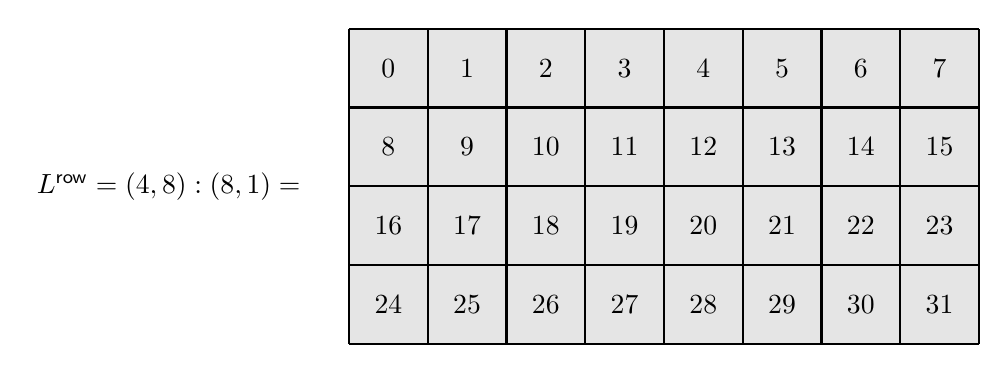
\begin{tikzpicture}[x={(0cm,-1cm)},y={(1cm,0cm)},every node/.style={minimum size=1cm, outer sep=0pt}]

\node[fill=gray!20] at (0,0) {0};
\node[fill=gray!20] at (0,1) {1};
\node[fill=gray!20] at (0,2) {2};
\node[fill=gray!20] at (0,3) {3};
\node[fill=gray!20] at (0,4) {4};
\node[fill=gray!20] at (0,5) {5};
\node[fill=gray!20] at (0,6) {6};
\node[fill=gray!20] at (0,7) {7};
\node[fill=gray!20] at (1,0) {8};
\node[fill=gray!20] at (1,1) {9};
\node[fill=gray!20] at (1,2) {10};
\node[fill=gray!20] at (1,3) {11};
\node[fill=gray!20] at (1,4) {12};
\node[fill=gray!20] at (1,5) {13};
\node[fill=gray!20] at (1,6) {14};
\node[fill=gray!20] at (1,7) {15};
\node[fill=gray!20] at (2,0) {16};
\node[fill=gray!20] at (2,1) {17};
\node[fill=gray!20] at (2,2) {18};
\node[fill=gray!20] at (2,3) {19};
\node[fill=gray!20] at (2,4) {20};
\node[fill=gray!20] at (2,5) {21};
\node[fill=gray!20] at (2,6) {22};
\node[fill=gray!20] at (2,7) {23};
\node[fill=gray!20] at (3,0) {24};
\node[fill=gray!20] at (3,1) {25};
\node[fill=gray!20] at (3,2) {26};
\node[fill=gray!20] at (3,3) {27};
\node[fill=gray!20] at (3,4) {28};
\node[fill=gray!20] at (3,5) {29};
\node[fill=gray!20] at (3,6) {30};
\node[fill=gray!20] at (3,7) {31};
\draw[color=black,thick,shift={(-0.5,-0.5)}] (0,0) grid (4,8);

\node[anchor=east] at (1.5,-1) {$L^\row = (4,8):(8,1) =$};
\end{tikzpicture}

\end{centering}

\bigskip

\noindent 记号 $L^\row = (4,8):(8,1)$ 表示矩阵第 $(i,j)$ 个元素的偏移为
\[
(i,j) \cdot (8,1) = 8i + j. 
\]

\noindent 另一种常见的选择是{\bf 列主序}（column-major）布局 \\

\begin{centering}

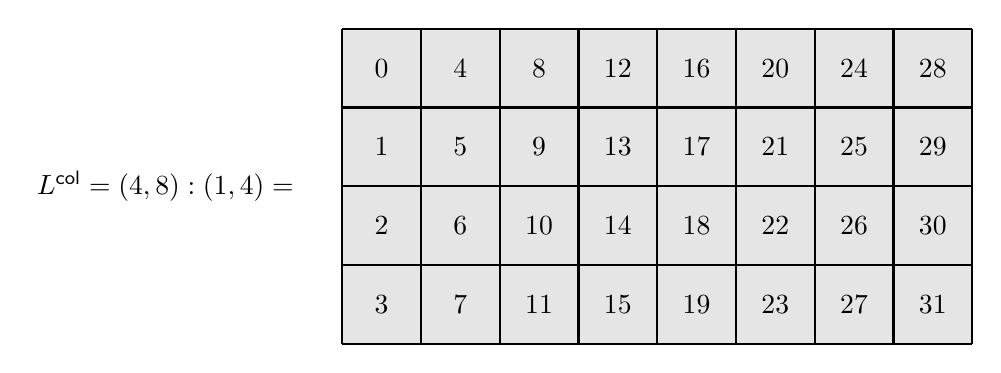
\begin{tikzpicture}[x={(0cm,-1cm)},y={(1cm,0cm)},every node/.style={minimum size=1cm, outer sep=0pt}]

\node[fill=gray!20] at (0,0) {0};
\node[fill=gray!20] at (0,1) {4};
\node[fill=gray!20] at (0,2) {8};
\node[fill=gray!20] at (0,3) {12};
\node[fill=gray!20] at (0,4) {16};
\node[fill=gray!20] at (0,5) {20};
\node[fill=gray!20] at (0,6) {24};
\node[fill=gray!20] at (0,7) {28};
\node[fill=gray!20] at (1,0) {1};
\node[fill=gray!20] at (1,1) {5};
\node[fill=gray!20] at (1,2) {9};
\node[fill=gray!20] at (1,3) {13};
\node[fill=gray!20] at (1,4) {17};
\node[fill=gray!20] at (1,5) {21};
\node[fill=gray!20] at (1,6) {25};
\node[fill=gray!20] at (1,7) {29};
\node[fill=gray!20] at (2,0) {2};
\node[fill=gray!20] at (2,1) {6};
\node[fill=gray!20] at (2,2) {10};
\node[fill=gray!20] at (2,3) {14};
\node[fill=gray!20] at (2,4) {18};
\node[fill=gray!20] at (2,5) {22};
\node[fill=gray!20] at (2,6) {26};
\node[fill=gray!20] at (2,7) {30};
\node[fill=gray!20] at (3,0) {3};
\node[fill=gray!20] at (3,1) {7};
\node[fill=gray!20] at (3,2) {11};
\node[fill=gray!20] at (3,3) {15};
\node[fill=gray!20] at (3,4) {19};
\node[fill=gray!20] at (3,5) {23};
\node[fill=gray!20] at (3,6) {27};
\node[fill=gray!20] at (3,7) {31};
\draw[color=black,thick,shift={(-0.5,-0.5)}] (0,0) grid (4,8);

\node[anchor=east] at (1.5,-1) {$L^\col = (4,8):(1,4) = $};
\end{tikzpicture}

\end{centering} 
\bigskip

\noindent 同样，记号 $L^\col = (4,8):(1,4)$ 表示矩阵第 $(i,j)$ 个元素的偏移为
\[
(i,j) \cdot (1,4) = i + 4j.
\]

\noindent 这些布局极其有用，但并不能满足所有目的。例如，在高性能计算中，人们常常通过如下步骤来计算矩阵乘积 $AB$：
\begin{enumerate}
    \item 把操作数矩阵 $A$ 与 $B$ 划分为若干瓦片（tile），
    \item 计算各瓦片之间的矩阵乘积，以及
    \item 合并这些部分结果以得到完整结果 $AB$。
\end{enumerate}
譬如，我们可以把 $4 \times 8$ 矩阵 $A$ 划分为 $2 \times 2$ 的瓦片，如下所示。
\[
A = \left[\begin{array}{cccc}
\begin{bmatrix}
12.47 & 87.21 \\
64.88 & 30.41 
\end{bmatrix}
&
\begin{bmatrix} 
34.08 & 56.93 \\
1.72 & 88.04 
\end{bmatrix}
&
\begin{bmatrix}
45.65 &  9.17 \\
92.55 & 17.06
\end{bmatrix}
&
\begin{bmatrix} 
73.02 & 21.39 \\
50.91 & 68.77
\end{bmatrix} 
\\[2ex]
\begin{bmatrix}
 3.33 & 77.19 \\
 91.40 & 26.12
\end{bmatrix} 
&
\begin{bmatrix} 
 61.58 & 29.46 \\
6.97 & 53.03 
\end{bmatrix}
&
\begin{bmatrix} 
 15.82 & 80.75 \\
58.66 & 33.79
\end{bmatrix} 
&
\begin{bmatrix} 
 44.62 & 39.28 \\
11.20 & 70.55
\end{bmatrix} 
\end{array}\right]
\]
% \noindent We can consider $A^\tiled$ as a tensor of shape $((2,2),(2,4))$, where 
% \[
% A^\tiled_{(i,j),(k,\ell)} = \begin{matrix}
%     \text{the }(i,j)\text{th entry of} \\
%     \; \;\text{the } (k,\ell)\text{th tile of }A.
% \end{matrix}
% \]

\noindent 现在假设我们想切出 $A$ 的各个瓦片，并设 $A$ 在内存中按列主序格式存放。为此，可以按如下方式手工计算偏移：对第 $(i,j)$ 个瓦片，索引其左上角元素的偏移由 $2i + 8j$ 给出。另一方面，为了更好地组织这一计算，我们可以使用瓦片的{\bf 交错}（interleaved）布局
\\


\begin{centering}

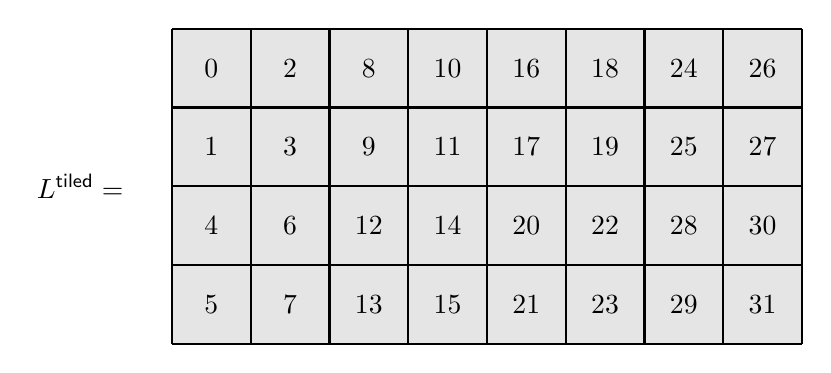
\begin{tikzpicture}[x={(0cm,-1cm)},y={(1cm,0cm)},every node/.style={minimum size=1cm, outer sep=0pt}]

\node[fill=gray!20]       at (0,0) {0};
\node[fill=gray!20]       at (0,1) {2};
\node[fill=gray!20]      at (0,2) {8};
\node[fill=gray!20]      at (0,3) {10};
\node[fill=gray!20]  at (0,4) {16};
\node[fill=gray!20]  at (0,5) {18};
\node[fill=gray!20]        at (0,6) {24};
\node[fill=gray!20]        at (0,7) {26};

\node[fill=gray!20]       at (1,0) {1};
\node[fill=gray!20]       at (1,1) {3};
\node[fill=gray!20]      at (1,2) {9};
\node[fill=gray!20]      at (1,3) {11};
\node[fill=gray!20]  at (1,4) {17};
\node[fill=gray!20]  at (1,5) {19};
\node[fill=gray!20]        at (1,6) {25};
\node[fill=gray!20]        at (1,7) {27};

\node[fill=gray!20]       at (2,0) {4};
\node[fill=gray!20]       at (2,1) {6};
\node[fill=gray!20]      at (2,2) {12};
\node[fill=gray!20]      at (2,3) {14};
\node[fill=gray!20]  at (2,4) {20};
\node[fill=gray!20]  at (2,5) {22};
\node[fill=gray!20]        at (2,6) {28};
\node[fill=gray!20]        at (2,7) {30};

\node[fill=gray!20]       at (3,0) {5};
\node[fill=gray!20]       at (3,1) {7};
\node[fill=gray!20]      at (3,2) {13};
\node[fill=gray!20]      at (3,3) {15};
\node[fill=gray!20]  at (3,4) {21};
\node[fill=gray!20]  at (3,5) {23};
\node[fill=gray!20]        at (3,6) {29};
\node[fill=gray!20]        at (3,7) {31};
\draw[color=black,thick,shift={(-0.5,-0.5)}] (0,0) grid (4,8);

\node[anchor=east] at (1.5,-1) {$L^\tiled =$};

% \node at (0,-1) {\Large{\texttt{0}}};
% \node at (1,-1) {\Large{\texttt{1}}};
% \node at (2,-1) {\Large{\texttt{2}}};
% \node at (3,-1) {\Large{\texttt{3}}};
% \node at (-1,0) {\Large{\texttt{0}}};
% \node at (-1,1) {\Large{\texttt{1}}};
% \node at (-1,2) {\Large{\texttt{2}}};
% \node at (-1,3) {\Large{\texttt{3}}};
% \node at (-1,4) {\Large{\texttt{4}}};
% \node at (-1,5) {\Large{\texttt{5}}};
% \node at (-1,6) {\Large{\texttt{6}}};
% \node at (-1,7) {\Large{\texttt{7}}};
\end{tikzpicture}

\end{centering}

\bigskip

\noindent 其中列由 $A$ 的瓦片给出，行由瓦片形状内的坐标给出。这里我们用{\bf 余字典序}（colexicographic ordering）来线性地枚举瓦片以及瓦片内的坐标，因此布局 $L^\tiled$ 的顶层形状为 $(4, 8)$。

然而，请注意，$L^\tiled$ 所呈现的交错模式意味着，对任何步长 $a,b$，它都不能表示为布局 $(4,8):(a,b)$。作为替代，我们可以把形状 $(4,8)$ 的各模式分解因式，并定义
\[ L^\tiled = ((2,2),(2,4)):((1,4),(2,8)). \]

\noindent 这样，前面的偏移计算 $2i + 8j$ 就体现为在坐标 $(0, (i,j))$ 上对 $L^\tiled$ 求值，而瓦片布局本身则由第一个模式给出。于是，在为 $A$ 赋予布局 $L^\tiled$ 而得到 $A^\tiled$ 之后，我们就可以把 $A$ 的第 $(i,j)$ 个瓦片取为切片

\[ A_{i,j} = A^\tiled(\; \rule{.7em}{0.4pt} \; , (i,j)). \]

CUTLASS 中发展的一个关键思想是：像 $L^\tiled$ 这样有用但更复杂的辅助布局，可以通过某些基本运算从更简单的布局系统地推导出来。就 $L^\tiled$ 而言，所涉及的运算称为{\bf 逻辑切分}（logical division）。若记
\\

\begin{centering}

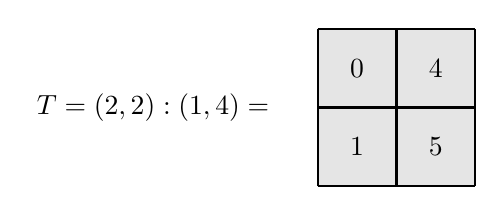
\begin{tikzpicture}[x={(0cm,-1cm)},y={(1cm,0cm)},every node/.style={minimum size=1cm, outer sep=0pt}]
\node[fill=gray!20]       at (0,0) {0};
\node[fill=gray!20]       at (1,0) {1};
\node[fill=gray!20]      at (0,1) {4};
\node[fill=gray!20]      at (1,1) {5};
\draw[color=black,thick,shift={(-0.5,-0.5)}] (0,0) grid (2,2);

\node[anchor=east] at (0.5,-1) {$T = (2,2):(1,4) =$};
\end{tikzpicture}

\end{centering}

\bigskip

\noindent 为瓦片布局，则 $L^\tiled$ 就是逻辑切分

\[
L^\tiled = L^\col \oslash T
\]
如下图所示。\\

\begin{centering}
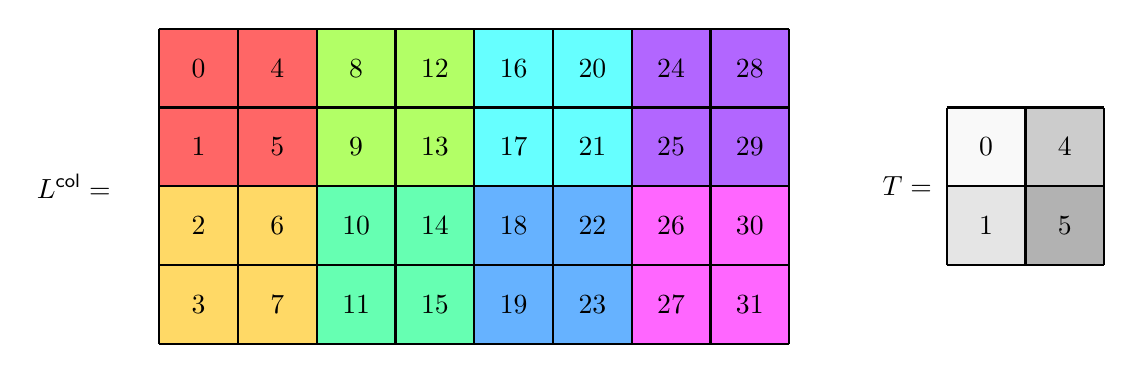
\begin{tikzpicture}[x={(0cm,-1cm)},y={(1cm,0cm)},every node/.style={minimum size=1cm, outer sep=0pt}]

\node[fill=colorx1!60] at (0,0) {0};
\node[fill=colorx1!60] at (0,1) {4};
\node[fill=colorx3!60] at (0,2) {8};
\node[fill=colorx3!60] at (0,3) {12};
\node[fill=colorx5!60] at (0,4) {16};
\node[fill=colorx5!60] at (0,5) {20};
\node[fill=colorx7!60] at (0,6) {24};
\node[fill=colorx7!60] at (0,7) {28};
\node[fill=colorx1!60] at (1,0) {1};
\node[fill=colorx1!60] at (1,1) {5};
\node[fill=colorx3!60] at (1,2) {9};
\node[fill=colorx3!60] at (1,3) {13};
\node[fill=colorx5!60] at (1,4) {17};
\node[fill=colorx5!60] at (1,5) {21};
\node[fill=colorx7!60] at (1,6) {25};
\node[fill=colorx7!60] at (1,7) {29};
\node[fill=colorx2!60] at (2,0) {2};
\node[fill=colorx2!60] at (2,1) {6};
\node[fill=colorx4!60] at (2,2) {10};
\node[fill=colorx4!60] at (2,3) {14};
\node[fill=colorx6!60] at (2,4) {18};
\node[fill=colorx6!60] at (2,5) {22};
\node[fill=colorx8!60] at (2,6) {26};
\node[fill=colorx8!60] at (2,7) {30};
\node[fill=colorx2!60] at (3,0) {3};
\node[fill=colorx2!60] at (3,1) {7};
\node[fill=colorx4!60] at (3,2) {11};
\node[fill=colorx4!60] at (3,3) {15};
\node[fill=colorx6!60] at (3,4) {19};
\node[fill=colorx6!60] at (3,5) {23};
\node[fill=colorx8!60] at (3,6) {27};
\node[fill=colorx8!60] at (3,7) {31};
\draw[color=black,thick,shift={(-0.5,-0.5)}] (0,0) grid (4,8);

\node[anchor = east] at (1.5,-1) {$L^\col = $ };
\node[anchor = east] at (1.5,9.5) {$T = $};

\node[fill=gray!5] at (1,10) {0};
\node[fill=gray!20] at (2,10) {1};
\node[fill=gray!40] at (1,11) {4};
\node[fill=gray!60] at (2,11) {5};
\draw[color=black,thick,shift={(-0.5,-0.5)}] (1,10) grid (3,12);
\end{tikzpicture}

\end{centering}

\vspace{0.2in}

\begin{centering}
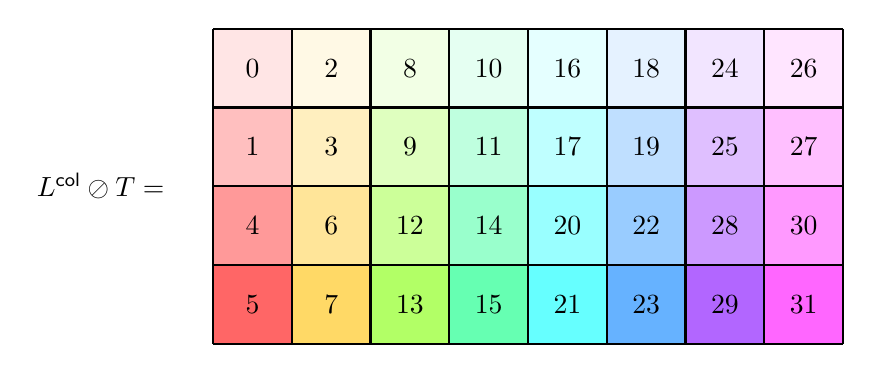
\begin{tikzpicture}[x={(0cm,-1cm)},y={(1cm,0cm)},every node/.style={minimum size=1cm, outer sep=0pt}]

\node[fill=colorx1!10]       at (0,0) {0};
\node[fill=colorx2!10]       at (0,1) {2};
\node[fill=colorx3!10]      at (0,2) {8};
\node[fill=colorx4!10]      at (0,3) {10};
\node[fill=colorx5!10]  at (0,4) {16};
\node[fill=colorx6!10]  at (0,5) {18};
\node[fill=colorx7!10]        at (0,6) {24};
\node[fill=colorx8!10]        at (0,7) {26};

\node[fill=colorx1!25]       at (1,0) {1};
\node[fill=colorx2!25]       at (1,1) {3};
\node[fill=colorx3!25]      at (1,2) {9};
\node[fill=colorx4!25]      at (1,3) {11};
\node[fill=colorx5!25]  at (1,4) {17};
\node[fill=colorx6!25]  at (1,5) {19};
\node[fill=colorx7!25]        at (1,6) {25};
\node[fill=colorx8!25]        at (1,7) {27};

\node[fill=colorx1!40]       at (2,0) {4};
\node[fill=colorx2!40]       at (2,1) {6};
\node[fill=colorx3!40]      at (2,2) {12};
\node[fill=colorx4!40]      at (2,3) {14};
\node[fill=colorx5!40]  at (2,4) {20};
\node[fill=colorx6!40]  at (2,5) {22};
\node[fill=colorx7!40]        at (2,6) {28};
\node[fill=colorx8!40]        at (2,7) {30};

\node[fill=colorx1!60]       at (3,0) {5};
\node[fill=colorx2!60]       at (3,1) {7};
\node[fill=colorx3!60]      at (3,2) {13};
\node[fill=colorx4!60]      at (3,3) {15};
\node[fill=colorx5!60]  at (3,4) {21};
\node[fill=colorx6!60]  at (3,5) {23};
\node[fill=colorx7!60]       at (3,6) {29};
\node[fill=colorx8!60]       at (3,7) {31};
\draw[color=black,thick,shift={(-0.5,-0.5)}] (0,0) grid (4,8);

\node[anchor=east] at (1.5,-1) {$ L^\col \oslash T = $};

% \node at (0,-1) {\Large{\texttt{0}}};
% \node at (1,-1) {\Large{\texttt{1}}};
% \node at (2,-1) {\Large{\texttt{2}}};
% \node at (3,-1) {\Large{\texttt{3}}};
% \node at (-1,0) {\Large{\texttt{0}}};
% \node at (-1,1) {\Large{\texttt{1}}};
% \node at (-1,2) {\Large{\texttt{2}}};
% \node at (-1,3) {\Large{\texttt{3}}};
% \node at (-1,4) {\Large{\texttt{4}}};
% \node at (-1,5) {\Large{\texttt{5}}};
% \node at (-1,6) {\Large{\texttt{6}}};
% \node at (-1,7) {\Large{\texttt{7}}};
\end{tikzpicture}

\end{centering}

\bigskip

除逻辑切分之外，其他基本的布局运算还包括{\bf 逻辑乘积}（logical product）、{\bf 补}（complement），以及最重要的{\bf 复合}（composition）。这些布局运算是 CUTLASS 的支柱，深入理解它们的行为有助于编写正确且高性能的代码。然而，这些运算的定义与构造相当精妙。例如，布局 $A$ 与 $B$ 的复合 $B \circ A$ 只有在 $A$ 与 $B$ 满足某些整除性约束时才是良定义（well-defined）的，CUTLASS 会在底层检查这些约束。特别地，两个布局何时可复合、以及应如何解释它们的复合，并不总是显然的。

% To support these tasks, NVIDIA's CUTLASS library provides a powerful toolkit for working with layouts. The core abstraction of the CUTLASS library is the {\bf CuTe layout}, or simply {\bf layout}, which specifies a logical-to-physical coordinate transformation (\cite{cutedsldocumentation}, \cite{cutedocumentation}). Throughout this work, we include code snippets written in NVIDIA’s CuTe DSL, a Python-based implementation of CuTe, which we refer to simply as $\texttt{cute}$. CuTe layouts and the operations which they support abstract away the complexity of layout management, allowing programmers to work with high-dimensional structures efficiently and intuitively. The power of layouts comes from the vast collection of operations they support.

% Given the subtlety of these operations, there is a clear need for a more accessible and mathematically grounded treatment of layouts.

% TODO: Get Cris Cecka consent or not to mention his forthcoming work.
% Mathematically, the theory of {\bf categories} and {\bf operads} provides a convenient language and set of standard mathematical tools for describing and reasoning about algebraic structures with a notion of composition. In this work, we will adopt a categorical perspective in order to develop one possible mathematical framework for CuTe layouts, although knowledge of category theory or operads isn't a strict prerequisite to read this work. We mention here that another framework has been developed in forthcoming work by Cris Cecka, the original author of CuTe, and the reader may wish to compare his perspective with ours.

\section{主要结果综述}

本文的主要思想是：通过把注意力限制在{\bf 可处理布局}（tractable layout）上——其元素满足一个简单的整除性条件（见定义 \ref{definitionoftractablelayouts}）——我们可以为布局的操纵发展出一套直观而强大的数学框架。可处理布局几乎涵盖了实践中会遇到的所有布局，例如
\begin{itemize}
\item {\it 行主序}与{\it 列主序}布局，它们无处不在；
\item {\it 紧凑}（compact）布局，它们把数据存储在连续的内存地址中；
\item {\it 投影}（projection）布局，它们广播数据的多个副本；以及
\item {\it 膨胀}（dilation）布局，它们支持带填充的加载与存储。
\end{itemize}
若 $L$ 是可处理布局，则我们可以用{\bf 图表}（diagram）来表示 $L$。例如，布局 $L^\row$、$L^\col$ 与 $L^\tiled$ 由下列图表表示。

\[\begin{tikzcd}[row sep = 1, column sep = 12]
  & & & &  & & 8 \ar[drr,mapsto] & & 4 \\
 (4,8):(8,1) & & \leftrightsquigarrow & &   & & 4 \ar[urr,mapsto] & & 8 \\
  & & & &  & &   & &  \\
 & & & &   & &   & &   \\[2em]
 & & & &   & &   & &  \\
 & & & &   & & 8 \ar[rr,mapsto] & & 8  \\
(4,8):(1,4)& & \leftrightsquigarrow& &   & & 4 \ar[rr,mapsto] & & 4  \\
  & & & &  & &   & &    \\
 & & & &   & &   & &   \\[2em]
 & & & &   & &   & &    \\
 & & & &  & & 4 \ar[rr,mapsto] & & 4  \\
& & & & 8 \ar[rr,-] \ar[urr,-] & & 2 \ar[drr,mapsto] & & 2 & & & & \\
 ((2,2),(2,4)):((1,4),(2,8)) & & \leftrightsquigarrow & &   & & 2 \ar[urr,mapsto] & & 2 \\
& & & & 4 \ar[urr,-] \ar[rr,-]  & & 2 \ar[rr,mapsto] & & 2  \\
& & & &   & &   & &   \\
\end{tikzcd}\]
% \[\begin{tikzcd}[row sep = 1, column sep = 8]
% & & & & & & & &  & & \\
% & & & & & & & & & & 4\\
%     (4,4) \ar[rrrr,"f"] \ar[rrrr,swap,"(1{,}3)"] & & & & (4,2,4)  & & \rightsquigarrow & & 4 \ar[urr,mapsto] & & 2\\
%     & & & & & & & & 4 \ar[rr,mapsto] & & 4\\
%     & & & & & & & &  & f &\\
% & & & & & & & & & & \\[2em]
% & & & & & & & & 2 \ar[drr,mapsto] & & 2\\
%     (2,2,2) \ar[rrrr,"g"] \ar[rrrr,swap,"(1{,}3{,}2)"] & & & & (2,2,2)  & & \rightsquigarrow & & 2 \ar[urr,mapsto] & & 2\\
%     & & & & & & & & 2 \ar[rr,mapsto] & & 2\\
%     & & & & & & & &  & g &
% & & & & & & & & & & \\[2em]
% & & & & & & & & 4 & & \\
% & & & & & & & & 4 \ar[drr,mapsto] & & \\
% & & & & & & & & 4 & & 4\\
%     (16,(4,4),(4,4)) \ar[rrrr,"h"] \ar[rrrr,swap,"(1{,}2{,}*{,}3{,}*)"] & & & & (16,4,4)  & & \rightsquigarrow & & 4 \ar[rr,mapsto] & & 4\\
%     & & & & & & & & 16 \ar[rr,mapsto] & & 16\\
%     & & & & & & & &  & h &
% \end{tikzcd}\]

\noindent 这些图表可以解释为某个{\bf 范畴}（category）中的态射（morphism）。这使我们得以借助{\bf 范畴论}（category theory）的力量来描述布局及其运算。\footnote{对于不熟悉这一学科的读者，我们在附录 \ref{categorytheoryappendix} 中提供了范畴论入门。}

更确切地说，我们定义一个范畴 $\catstyle{Nest}$，其对象（object）是正整数的嵌套元组（nested tuple），其态射 $f:S \to T$ 对应于如上那种图表（详见定义 \ref{definitionofTuple} 与定义 \ref{definitionofNest}）。若 $L$ 是{\bf 非退化}（non-degenerate）的可处理布局（见定义 \ref{definitionofnondegeneratelayout}），则存在一个本质唯一的 $\catstyle{Nest}$-态射 $f$ 编码 $L$，正如下面的对应定理所展示的那样。
% An object of $\catstyle{Nest}$ is a nested tuples of positive integers, and a morphism $f:S \to T$ in $\catstyle{Nest}$ associates entries of $S$ to entries of $T$ (see Definition \ref{definitionofTuple} and Definition \ref{definitionofNest}). If $f:S \to T$ is a nested tuple morphism, then $f$ encodes a tractable layout $L_f$. The shape of $L_f$ is $S$, and the stride of $L_f$ is a nested tuple whose entries are certain prefix products of $T$ (See Construction \ref{layoutfromnestedtuplemorphism}). For example, the layouts encoded by the morphisms $f$, $g$, and $h$ above are
% \begin{align*}
%     L_f & = (4,4):(1,8)\\
%     L_g & = (2,2,2):(1,4,2)\\
%     L_h & = (16,(4,4),(4,4)): (1,(16,0),(64,0)).
% \end{align*}

 % Conversely, if $L$ is a tractable layout, then there exists a nested tuple morphism $f_L$ which encodes $L$. The nested tuple morphism which encodes $L$ is not unique. However, we introduce a notion of {\it standard form} for nested tuple morphisms (Definition \ref{definitionofnestedstandardform}), and prove the following correspondence theorem.
\begin{mainthm}(参见 \ref{nestedonetoonecorrespondence})
存在一一对应
    \[ \begin{tikzcd} 
    \begin{Bmatrix}
    \text{非退化}\\
        \text{可处理布局}
    \end{Bmatrix} 
    \ar[r] & \ar[l] 
        \begin{Bmatrix}
        \text{非退化}\\
        \catstyle{Nest}\text{-态射}\\
        \text{（标准形式）}
    \end{Bmatrix}
    \end{tikzcd} 
    \]
\end{mainthm}

诸如复合、逻辑切分与逻辑乘积这样的布局运算，都可以在范畴 $\catstyle{Nest}$ 中得到自然的解释。若
\[
\begin{tikzcd}
    S \ar[r,"f"]  & T \ar[r,"g"]  & U
\end{tikzcd}
\]
是 $\catstyle{Nest}$-态射，则我们可以通过把相应的图表粘合在一起来构成复合
\[\begin{tikzcd}
S \ar[r,"g \circ f"] &  U
\end{tikzcd} \]
例如，
% \[\begin{tikzcd}
% (2,2) \ar[rr,"f"] \ar[rr,swap,"(2{,}1)"] & & (2,2) \ar[rr,"g"] \ar[rr,swap,"(2{,}3)"] & & (5,(2,2))
% \end{tikzcd}\]
% is 
% \[\begin{tikzcd}
% (2,2) \ar[rr,"g \circ f"] \ar[rr,swap,"(3{,}2)"] & &  (5,(2,2))
% \end{tikzcd}\]
% as depicted below.
\[ \begin{tikzcd}[row sep = 1, column sep = 8]
 & &   & & 2 & & & & & & 2\\
2 \ar[drr,mapsto]  & & 2 \ar[urr,mapsto] & & 2 & & \rightsquigarrow & & 2 \ar[rr,mapsto]  & & 2\\
2 \ar[urr,mapsto] & & 2 \ar[urr,mapsto] & & 5 & & & & 2 \ar[uurr,mapsto] & & 5\\
 & f & & g & & & & & & \mathclap{g \circ f} & 
\end{tikzcd}\]
我们证明 $\catstyle{Nest}$ 中的复合与布局复合相容。
\begin{mainthm}(参见 \ref{compatibilityofcompositioninD}) 若 $f$ 与 $g$ 是非退化的、可复合的 $\catstyle{Nest}$-态射，则
\[
L_{g \circ f} = L_g \circ L_f.
\]
\end{mainthm}
% For example, if $f$ and $g$ are the morphisms above, then 
% \begin{align*}
%     L_f & =(2,2):(2,1) \\
%     L_g & = (2,2):(5,10)\\
%     L_{g \circ f} & = (2,2):(10,5)\\
%     L_g \circ L_f& = (2,2):(10,5).
% \end{align*}

我们可以通过折叠相邻的箭头来合并（coalesce）$\catstyle{Nest}$-态射 $f$。例如，
% on nested tuple morphisms.
% For example if $f$ is the morphism 
% \[
% \begin{tikzcd} 
% ((2,2),(10,10)) \ar[rr,"f"] \ar[rr,swap,"(1{,}2{,}4{,}5)"] & & (2,2,2,10,10)
% \end{tikzcd}
% \]
% then $\coalesce(f)$ is the morphism 
% \[
% \begin{tikzcd} 
% (4,100) \ar[rr,"\coalesce(f)"] \ar[rr,swap,"(1{,}3)"] & & (4,2,100)
% \end{tikzcd}
% \]
% as depicted below.
\[\begin{tikzcd}[row sep = 1, column sep = 8]
 & & 10 & & & & & & \\
 10 \ar[urr,mapsto] & & 10 & & & & & & \\
 10 \ar[urr,mapsto] & & 2 & & & & & & 100\\
 2 \ar[rr,mapsto] & & 2 & & \rightsquigarrow & & 100 \ar[urr,mapsto] & & 2\\
 2 \ar[rr,mapsto] & & 2 & & & & 4 \ar[rr,mapsto] & & 4\\
    & f & & & & & & \mathclap{\coalesce(f)} & 
\end{tikzcd}\]
我们证明该运算与布局的合并运算相容。
\begin{mainthm}(参见 \ref{coalesceagreement}) 若 $f$ 是 $\catstyle{Nest}$-态射，则
\[
L_{\coalesce(f)} = \coalesce(L_f).
\]
\end{mainthm}
% For example, if $f$ is the morphism above, then 
% \begin{align*}
%     L_f & = ((2,2),(10,10)):((1,2),(8,80))\\
%     L_{\coalesce(f)} & = (4,100):(1,8)\\
%     \coalesce(L_f) & = (4,100):(1,8).
% \end{align*}

$\catstyle{Nest}$-态射 $f$ 的补是未被 $f$ 命中的元素所构成的包含映射（inclusion）。例如，
% if $f$ is the morphism 
% \[
% \begin{tikzcd} 
% (2,2) \ar[rr,"f"] \ar[rr,swap,"(1{,}3)"] & & (2,5,2,5)
% \end{tikzcd}
% \]
% then $f^c$ is the morphism 
% \[
% \begin{tikzcd} 
% (5,5) \ar[rr,"f^c"] \ar[rr,swap,"(2{,}4)"] & & (2,5,2,5)
% \end{tikzcd}
% \]
% as depicted below.
\[\begin{tikzcd}[row sep = 1, column sep = 8]
 & & 5 & & & & & & 5\\
 & & 2 & & & & & & 2\\
 2 \ar[urr,mapsto] & & 5 & & \rightsquigarrow &  & 5 \ar[uurr,mapsto] & & 5\\
 2 \ar[rr,mapsto] & & 2 & & & &  5 \ar[urr,mapsto]  & & 2\\
    & f & & & & & &  f^c & 
\end{tikzcd}\]
我们证明 $\catstyle{Nest}$ 中的补与布局的补相容。
\begin{mainthm}(参见 \ref{coalescedlayoutoftuplemorphismcomplement}) 若 $f:S \to T$ 是单射的 $\catstyle{Nest}$-态射且 $N = \size(T)$，则
\[
\coalesce(L_{f^c}) = \comp(L_f,N).
\]
\end{mainthm} 
% For example, if $f$ is the morphism above, then 
% \begin{align*}
% L_f & = (2,2):(1,10)\\
% L_{f^c} & = (5,5):(2,20)\\
% \comp(L_f,100)&  = (5,5):(2,20).
% \end{align*}

我们定义 $\catstyle{Nest}$-态射的整除性，以及当 $g$ 整除 $f$ 时的逻辑切分运算
\[
f,g \mapsto f \oslash g
\]
例如，
% if $f$ and $g$ are the morphisms 
% \[\begin{tikzcd}
%     ((4,8),(4,8)) \ar[rr,"f"] \ar[rr,swap,"(1{,}2{,}3{,}4)"] & & ((4,8),(4,8))\\
%     (4,4) \ar[rr,"g"] \ar[rr,swap,"(1{,}3)"] & & ((4,8),(4,8))
% \end{tikzcd}\]
% then $g$ divides $f$, and $f \oslash g$ is the morphism 
% \[\begin{tikzcd}
%     ((4,4),(8,8)) \ar[rr,"f\oslash g"] \ar[rr,swap,"(1{,}3{,}2{,}4)"] & & ((4,8),(4,8))
% \end{tikzcd}\]
% as depicted below.
\[\begin{tikzcd}[row sep = 1, column sep = 8]
  & & 8 \ar[rr,mapsto] & & 8 & & & & & &  8 \ar[rr,mapsto]  & & 8\\
  & & 4 \ar[rr,mapsto] & & 4 & & & & 64 \ar[rr,-] \ar[urr,-]& &  8 \ar[drr,mapsto] & & 4\\
4 \ar[urr,mapsto] & & 8 \ar[rr,mapsto] & & 8 & & \rightsquigarrow & &  & &  4 \ar[urr,mapsto] & & 8\\
4 \ar[rr,mapsto] & & 4 \ar[rr,mapsto] & & 4 & & & & 16 \ar[rr,-] \ar[urr,-]& & 4 \ar[rr,mapsto] & & 4\\
  & g &  & f & & & & & & & & \mathclap{f \oslash g} & 
\end{tikzcd}\]

我们证明 $\catstyle{Nest}$ 中的逻辑切分与布局的逻辑切分相容。
\begin{mainthm}(参见 \ref{coalesceoflogicaldivision}) 若 $f$ 与 $g$ 是非退化 $\catstyle{Nest}$-态射且 $g$ 整除 $f$，则
\[
\coalesce(L_{f \oslash g}) = \coalesce(L_f \oslash L_g).
\]
\end{mainthm}
% For example, if $f$ and $g$ are the morphisms above, then 
% \begin{align*}
%     L_f & = (4,8,4,8):(1,4,32,128)\\
%     L_g & = (4,4):(1,32)\\
%     L_{f \oslash g} & = ((4,4),(8,8)):((1,32),(4,128))\\
%     L_f \oslash L_g & = ((4,4),(8,8)):((1,32),(4,128)).
% \end{align*}

我们定义 $\catstyle{Nest}$-态射的乘积可许性（product admissibility），以及当 $f$ 与 $g$ 乘积可许时的逻辑乘积运算
\[
f,g \mapsto f \otimes g
\]
例如，
% if $f$ and $g$ are the nested tuple morphisms 
% \[\begin{tikzcd}
%     (2,2) \ar[rr,"f"] \ar[rr,swap,"(1{,}2)"] & & (2,2,5,5)\\
%     (5,5) \ar[rr,"g"] \ar[rr,swap,"(2{,}1)"] & & (5,5)
% \end{tikzcd}\]
% then $f$ and $g$ are product admissible, and $f \otimes g$ is the morphism 
% \[\begin{tikzcd}
%     ((2,2),(5,5)) \ar[rr,"f\oslash g"] \ar[rr,swap,"(1{,}2{,}4{,}3)"] & & (2,2,5,5)
% \end{tikzcd}\]
% as depicted below.
\[\begin{tikzcd}[row sep = 1, column sep = 8]
  & & 5 & &   & &  & &  & & & & 5 \ar[drr,mapsto] & & 5\\
  & & 5 & &   & & & & & & 25 \ar[rr,-] \ar[urr,-] & & 5 \ar[urr,mapsto] & & 5\\
2  \ar[rr,mapsto] & & 2 & & 5  \ar[drr,mapsto] & & 5 & & \rightsquigarrow & & &  & 2 \ar[rr,mapsto] & & 2\\
2 \ar[rr,mapsto] & & 2 & & 5 \ar[urr,mapsto]  & & 5 & & & & 4 \ar[rr,-] \ar[urr,-] & & 2 \ar[rr,mapsto] & & 2\\
  & f & & &  & g & & & & & & & & \mathclap{f \otimes g} & 
\end{tikzcd}\] 


我们证明 $\catstyle{Nest}$ 中的逻辑乘积与布局的逻辑乘积相容。
\begin{mainthm}(参见 \ref{logicalproductcompatibility}) 若 $f$ 与 $g$ 是非退化 $\catstyle{Nest}$-态射且二者乘积可许，则
\[
L_{f \otimes g} = L_f \otimes L_g.
\]
\end{mainthm}
% For example, if $f$ and $g$ are the morphisms above, then 
% \begin{align*}
%     L_f & = (2,2):(1,2)\\
%     L_g & = (5,5):(5,1) \\
%     L_{f \otimes g} & = ((2,2),(5,5)):((1,2),(20,4))\\
%     L_f \otimes L_g & = ((2,2),(5,5)):((1,2),(20,4))
% \end{align*}

在第 \ref{computationschapter} 章中，我们展示如何用我们的新框架来计算复合、逻辑切分与逻辑乘积等重要布局运算。特别地，我们给出一个计算可处理布局 $A$ 与 $B$ 的复合 $B \circ A$ 的算法（算法 \ref{tractablelayoutcompositionalgorithm}）。略去细节，我们算法的基本思想是：若要计算复合 $B \circ A$，可以用适当选取的 $\catstyle{Nest}$-态射 $f$ 与 $g$ 分别表示 $A$ 与 $B$，把这两个态射复合成 $g \circ f$，再取其编码的布局，从而得到
\[
B \circ A = L_{g \circ f}.
\]
我们用大量例子演示这一算法。

\section{结构安排}

本文的组织结构如下。 

在 \ref{implementationsection} 节中，我们给出布局的 $\texttt{cute}$ 实现的相关细节。我们以模块 $\texttt{tract}$ 的形式提供了范畴 $\catstyle{Nest}$ 的一个 Python 实现，并演示 $\texttt{tract}$ 与 $\texttt{cute}$ 的相容性。我们的 Python 实现可在我们的 git 仓库 \url{https://github.com/ColfaxResearch/layout-categories} 找到。

第 \ref{layoutschapter} 章是关于布局及其代数的全面参考。该章给出布局及其所支持运算的严格定义，并建立这些运算的基本性质。该章富含例子，对一线程序员也可能颇有助益。 

在第 \ref{categorieschapter} 章中，我们提出一个处理可处理布局的新数学框架。特别地，我们把布局及其代数与{\bf 范畴}和 {\bf operad} 的理论联系起来。该章内容具有独立的数学趣味，同时也有实用价值：它为可视化布局以及计算布局的各种运算提供了一个新框架。  

在第 \ref{computationschapter} 章中，我们利用第 \ref{categorieschapter} 章发展的框架，给出一个计算可处理布局 $A$ 与 $B$ 的复合的算法。我们用大量例子演示该复合算法。

\section{相关工作}

虽然本文在性质上是理论性的，但其动机来自 GPU 编程中的实际应用，最著名的当属 CUTLASS。我们强调，这里发展的理论是独立于实现的：它不依赖于在实践中用来实现布局的具体编程语言或运行时系统。尽管如此，在使用具体实现时仍会出现一些实际的考量。例如，CUTLASS 会区分编译期常量（静态变量）与运行时值（动态变量）。这一信息使编译器能够在代码生成期间进行优化。这类与实现相关的细节虽然对性能很重要，但超出了我们数学框架的讨论范围。进一步的讨论见 CuTe 文档 \cite{cutedocumentation}。

我们为布局发展的数学框架与计算机科学和数学的若干领域都有关联。我们简要回顾 GPU 编程及相邻领域的相关工作，以便为我们的贡献提供更完整的背景。

\begin{itemize}
    \item {\bf CUTLASS 的应用。}CUTLASS 的最先进应用包括 FlashAttention \cite{dao2023flashattention2, shah2024flashattention3}、EVT \cite{chen2024evt} 与 SonicMoE \cite{sonic}。对于希望更深入地理解 CUTLASS 与 CuTe 实际应用的读者，我们推荐 NVIDIA~\cite{cecka2024cutlass, sun2025cutlass, thakkar2025cutlass} 与 Colfax Research~\cite{shah2024cutlass_streamk, shah2025cutlass_blackwell_tensor_memory, shah2025cutlass_blackwell_clusters, shah2025cutlass_blackwell_subbyte} 关于用这些库进行 GPU 编程的系列综合教程。
    \item {\bf 数据布局优化} 数据布局优化技术通过仔细考量张量在内存中的存储方式，来改善缓存局部性与内存访问模式 \cite{xu2023alt, bacon1994compiler, raman2007structure, ju1992reduction}，\cite{sharma2015data}。选择高效的内存存储与访问模式对 GPU 性能至关重要，因为内存带宽往往正是瓶颈所在。
    \item {\bf 现代布局系统} CuTe \cite{cutedocumentation, cutedsldocumentation, shah2024layout} 与 Triton Linear Layouts \cite{tritonlinearlayouts, zhou2026linear} 等布局系统已成为张量计算中管理内存存储与访问的行业标准。Triton 线性布局基于 $\mathbb{F}_2$-线性代数，并从 $\mathbb{F}_2$-线性算子的复合继承复合结构。它们还与布局 swizzle 自然相容，而后者一般无法表示为 CuTe 布局。另一方面，这些布局不如 CuTe 布局富有表达力，因为它们的大小与余大小必须等于 $2$ 的幂，而且无法表达诸如乘以非 $2$ 的幂整数之类的变换。最近的研究表明，这两种布局系统都可以用整数集合关系来表达 \cite{bhaskaracharya2025}。这为统一处理 CuTe 布局、Triton 线性布局以及更一般的布局（例如具有非矩形形状的布局）提供了共同基础。
    
    \item {\bf 多面体编译} 多面体模型（polyhedral model）\cite{verdoolaege2010isl}，\cite{verdoolaege2021presburger}，\cite{thangamani2024survey} 为分析与变换具有仿射边界和数组访问的循环嵌套提供了数学框架。该模型的主要抽象，是把迭代空间表示为某个多面体中整点的集合。这一形式化方法允许进行复杂的循环变换，在优化局部性与并行性的同时保持程序语义。Pluto \cite{bondhugula2008pluto}、Polly \cite{grosser2012polly} 与 Tensor Comprehensions \cite{vasilache2018tensor} 等工具利用多面体技术自动生成优化代码。
    \item {\bf 张量缩并/分解} 张量缩并（tensor contraction）\cite{ShiNiranjanAnandkumarCecka2016, zhao2022polyhedral, KoldaBader2009} 把矩阵乘法推广到更高秩的张量，在机器学习与科学计算中无处不在。张量缩并的高效实现依赖于缩并次序与中间张量布局的最优选择。  
\end{itemize}

\clearpage

\section{实现} \label{implementationsection}
本节演示如何在 NVIDIA 的 CuTe DSL（我们将其记作 $\texttt{cute}$）中使用布局。我们在 git 仓库 \url{https://github.com/ColfaxResearch/layout-categories} 中以 $\texttt{Python}$ 模块 $\texttt{tract}$ 的形式给出了我们范畴框架的一个实现。这里我们展示 $\texttt{cute}$ 与 $\texttt{tract}$ 的相容性。

\begin{enumerate}[left=0pt]
\item {\bf 构造元组与嵌套元组：}我们在 \texttt{Python} 中如下构造元组（tuple）与嵌套元组。 
\begin{lstlisting}[language=cutedsl]
S = (2,2,2)
T = ((2,2),(5,5))
U = ((2,2),4,(9,(3,3)))
\end{lstlisting}
注意，若要构造长度为 $1$ 的元组，必须在元组的元素后面加上一个逗号。例如，
\begin{lstlisting}[language=cutedsl]
S = (10,)
T = (10)
\end{lstlisting}
返回
\begin{lstlisting}[language=cutedsl]
S = (10,)
T = 10
\end{lstlisting}
\item {\bf 构造布局与态射：}我们在 $\texttt{cute}$ 中如下构造布局
\[
L = S:D
\]
：
\begin{lstlisting}[language=cutedsl]
L = cute.make_layout(shape=S, stride=D)
\end{lstlisting}
例如，
\begin{lstlisting}[language=cutedsl]
A = cute.make_layout(shape=((4,4),4), stride=((16,1),4))
B = cute.make_layout(shape=(8,64), stride=(64,1))
C = cute.make_layout(shape=100, stride=2)
\end{lstlisting}
返回
\begin{lstlisting}[language=cutedsl]
A = ((4,4),4):((16,1),4)
B = (8,64):(64,1)
C = 100:2
\end{lstlisting}
我们在 $\texttt{tract}$ 中如下构造嵌套元组态射
\[\begin{tikzcd} 
S \ar[r,"f"] \ar[r,swap,"\alpha"] & T
\end{tikzcd} \]
：
\begin{lstlisting}[language=cutedsl]
f = tract.make_morphism(domain=S, codomain=T, map_=alpha)
\end{lstlisting}
例如，
\begin{lstlisting}[language=cutedsl]
f = tract.make_morphism(domain=(4,4), codomain=(4,2,4), map_=(1,3))
g = tract.make_morphism(domain=(2,2,2,2), codomain=(2,2,2,2), map_=(1,0,4,2))
h = tract.make_morphism(domain=(16,(4,4),(4,4)), codomain=(16,4,4), map_=(1,2,0,3,0))
\end{lstlisting}
返回
\begin{lstlisting}[language=cutedsl]
f = (4,4)--(1,3)-->(4,2,4)
g = (2,2,2,2)--(1,0,4,2)-->(2,2,2,2)
h = (16,(4,4),(4,4))--(1,2,0,3,0)-->(16,4,4)
\end{lstlisting}
注意，在 \texttt{tract} 中指定映射时，我们使用符号 \texttt{0} 而不是 $\ast$。

\item {\bf 在可处理布局与态射之间转换：}
若 $L$ 是布局，我们可以用如下方式检查 $L$ 是否可处理：
\begin{lstlisting}[language=cutedsl]
tract.is_tractable(L)
\end{lstlisting}
例如，
\begin{lstlisting}[language=cutedsl]
A = cute.make_layout(shape=(2,2,2), stride=(1,2,4))
B = cute.make_layout(shape=(2,2,2), stride=(1,7,4))
A_is_tractable = tract.is_tractable(A)
B_is_tractable = tract.is_tractable(B)
\end{lstlisting}
返回
\begin{lstlisting}[language=cutedsl]
A = (2,2,2):(1,2,4)
B = (2,2,2):(1,7,4)
A_is_tractable = True
B_is_tractable = False
\end{lstlisting}
若 $L$ 是可处理布局，则我们可以如下构造标准表示 $f_L$：
\begin{lstlisting}[language=cutedsl]
tract.compute_morphism(L)
\end{lstlisting}
例如，
\begin{lstlisting}[language=cutedsl]
L = cute.make_layout(shape=(2,2,2), stride=(1,2,4))
f_L = tract.compute_morphism(L)
\end{lstlisting}
返回
\begin{lstlisting}[language=cutedsl]
L = (2,2,2):(1,2,4)
f_L = (2,2,2)--(1,2,3)-->(2,2,2)
\end{lstlisting}
若 $f$ 是嵌套元组态射，我们可以如下构造由 $f$ 编码的布局 $L_f$：
\begin{lstlisting}[language=cutedsl]
tract.compute_layout(f)
\end{lstlisting}
例如，
\begin{lstlisting}[language=cutedsl]
f = tract.make_morphism(domain=((5,5),8), codomain=(5,8,5), map_=(1,3,2))
L_f = tract.compute_layout(f)
\end{lstlisting}
返回
\begin{lstlisting}[language=cutedsl]
f = ((5,5),8)--(1,3,2)-->(5,8,5)
L_f = ((5,5),8):((1,40),5)
\end{lstlisting}

\item {\bf 复合}：当有定义时，该运算从一对布局 $A$ 与 $B$ 产生布局 $B \circ A$。精确定义见定义 \ref{definitionoflayoutcomposition}。我们可以在 $\texttt{cute}$ 中如下计算复合 $B \circ A$：
\begin{lstlisting}[language=cutedsl]
cute.composition(B,A)
\end{lstlisting}
例如，运行
\begin{lstlisting}[language=cutedsl]
A = cute.make_layout(shape=((4,4),4), stride=((16,1),4))
B = cute.make_layout(shape=(8,64), stride=(64,1))
B_o_A = cute.composition(B,A)
\end{lstlisting}
返回
\begin{lstlisting}[language=cutedsl]
A = ((4,4),4):((16,1),4)
B = (8,64):(64,1)
B_o_A = ((4,4),(2,2)):((2,64),(256,1))
\end{lstlisting}
若 $f$ 与 $g$ 是可复合的嵌套元组态射，我们可以在 $\texttt{tract}$ 中如下计算复合 $g \circ f$：
\begin{lstlisting}[language=cutedsl]
tract.compose(f,g)
\end{lstlisting}
例如，
\begin{lstlisting}[language=cutedsl]
f = tract.make_morphism(domain=((2,2),(2,2)), codomain=((2,2,2),(2,2,2)), map_=(3,2,6,5))
g = tract.make_morphism(domain=((2,2,2),(2,2,2)), codomain=(2,2,2,2), map_=(1,0,2,0,3,4))
g_o_f = tract.compose(f,g)
\end{lstlisting}
返回
\begin{lstlisting}[language=cutedsl]
f = ((2,2),(2,2))--(3,2,6,5)-->((2,2,2),(2,2,2))
g = ((2,2,2),(2,2,2))--(1,0,2,0,3,4)-->(2,2,2,2)
g_o_f = ((2,2),(2,2))--(2,0,4,3)-->(2,2,2,2)
\end{lstlisting}

\item {\bf 合并}：该运算从布局 $A$ 产生布局 $\coalesce(A)$。详见定义 \ref{definitionofnestedlayoutcoalesce}。我们可以在 $\texttt{cute}$ 中如下计算 $\coalesce(A)$：
\begin{lstlisting}[language=cutedsl]
cute.coalesce(A)
\end{lstlisting}
例如，
\begin{lstlisting}[language=cutedsl]
A = cute.make_layout(shape = ((2,2),(2,2),(5,5)), stride = ((1,2),(16,32),(64,640)))
coal_A = cute.coalesce(A)
\end{lstlisting}
返回
\begin{lstlisting}[language=cutedsl]
A = ((2,2),(2,2),(5,5)):((1,2),(16,32),(64,640))
coal_A = (4,20,5):(1,16,640)
\end{lstlisting}
另外还有一个{\it 相对合并}（relative coalesce）运算 $A \mapsto \coalesce(A,S)$，它额外接收一个嵌套元组 $S$ 作为输入，且 $S$ 被 $A$ 的形状所{\it 加细}（refine）。详见定义 \ref{definitionofrelativecoalesce}。我们可以在 $\texttt{cute}$ 中如下计算 $\coalesce(A,S)$：
\begin{lstlisting}[language=cutedsl]
A = cute.make_layout(shape = ((2,2),(3,3),(5,5)), stride = ((1,2),(4,12),(36,180)))
S = ((2,2),9,25)
coal_A_over_S = cute.coalesce(A,target_profile=S)
\end{lstlisting}
返回
\begin{lstlisting}[language=cutedsl]
A = ((2,2),(3,3),(5,5)):((1,2),(4,12),(36,180))
S = ((2,2),9,25)
coal_A_over_S = ((2,2),9,25):((1,2),4,36)
\end{lstlisting}
若 $f$ 是嵌套元组态射，我们可以构造 $\coalesce(f)$。详见定义 \ref{definitionofcoalesceofnestedtuplemorphism}。我们在 $\texttt{tract}$ 中如下计算 $\coalesce(f)$：
\begin{lstlisting}[language=cutedsl]
tract.coalesce(f)
\end{lstlisting}
例如，
\begin{lstlisting}[language=cutedsl]
f = tract.make_morphism(domain=(2,2,10,10), codomain = (2,2,2,10,10), map_=(1,2,4,5))
coal_f = tract.coalesce(f)
\end{lstlisting}
返回
\begin{lstlisting}[language=cutedsl]
f = (2,2,10,10)--(1,2,4,5)-->(2,2,2,10,10)
coal_f = (4,100)--(1,3)-->(4,2,100)
\end{lstlisting}

\item {\bf 补}：当有定义时，该运算从布局 $A$ 与正整数 $N$ 产生布局 $\comp(A,N)$。详见定义 \ref{definitionoflayoutcomplements}。我们可以在 $\texttt{cute}$ 中如下计算 $\comp(A,N)$：
\begin{lstlisting}[language=cutedsl]
cute.complement(A,N)
\end{lstlisting}
例如，
\begin{lstlisting}[language=cutedsl]
A = cute.make_layout(shape = ((2,2),(2,2)), stride = ((8,2),(64,256)))
comp_A = cute.complement(A,4096)
\end{lstlisting}
返回
\begin{lstlisting}[language=cutedsl]
A = ((2,2),(2,2)):((8,2),(64,256))
comp_A = (2,2,4,2,8):(1,4,16,128,512)
\end{lstlisting}
若 $f$ 是嵌套元组态射，则我们可以构造 $f$ 的补 $f^c$。详见定义 \ref{complementofmorphisminD}。我们在 $\texttt{tract}$ 中如下计算 $f^c$：
\begin{lstlisting}[language=cutedsl]
tract.complement(f)
\end{lstlisting}
例如，
\begin{lstlisting}[language=cutedsl]
f = tract.make_morphism(domain=(2,2), codomain=(2,5,2,5), map_=(1,3))
comp_f = tract.complement(f)
\end{lstlisting}
返回
\begin{lstlisting}[language=cutedsl]
f = (2,2)--(1,3)-->(2,5,2,5)
comp_A = (5,5)--(2,4)-->(2,5,2,5)
\end{lstlisting}
\item {\bf 逻辑切分}：当有定义时，该运算从一对布局 $A$ 与 $B$ 产生布局 $A \oslash B$。详见定义 \ref{definitionoflogicaldivide}。我们在 $\texttt{cute}$ 中如下计算 $A \oslash B$：
\begin{lstlisting}[language=cutedsl]
cute.logical_divide(A,B)
\end{lstlisting}
例如，
\begin{lstlisting}[language=cutedsl]
A = cute.make_layout((64,32), stride = (32,1))
B = cute.make_layout((4,4), stride = (1,64))
quotient = cute.logical_divide(A,B)
\end{lstlisting}
返回
\begin{lstlisting}[language=cutedsl]
A = (64,32):(32,1)
B = (4,4):(1,64)
quotient = ((4,4),(16,8)):((32,1),(128,4))
\end{lstlisting}
若 $f$ 与 $g$ 是嵌套元组态射且 $g$ 整除 $f$，则我们可以构造逻辑切分 $f \oslash g$。详见定义 \ref{definitionoflogicaldivisionofnestedtuplemorphisms}。我们在 $\texttt{tract}$ 中如下计算 $f \oslash g$：
\begin{lstlisting}[language=cutedsl]
tract.logical_divide(f,g)
\end{lstlisting}
例如，
\begin{lstlisting}[language=cutedsl]
f = tract.make_morphism(domain=(4,8,4,8), codomain=(4,8,4,8), map_=(1,2,3,4))
g = tract.make_morphism(domain=(4,4), codomain=(4,8,4,8), map_=(1,3))
quotient = tract.logical_divide(f,g)
\end{lstlisting}
返回
\begin{lstlisting}[language=cutedsl]
f = (4,8,4,8)--(1,2,3,4)-->(4,8,4,8)
g = (4,4)--(1,3)-->(4,8,4,8)
quotient = ((4,4),(8,8))--(1,3,2,4)-->(4,8,4,8)
\end{lstlisting}
\item {\bf 逻辑乘积}：当有定义时，该运算从一对布局 $A$ 与 $B$ 产生布局 $A \otimes B$。详见定义 \ref{definitionoflogicalproduct}。我们在 $\texttt{cute}$ 中如下计算 $A \otimes B$：
\begin{lstlisting}[language=cutedsl]
cute.logical_product(A,B)
\end{lstlisting}
例如，运行
\begin{lstlisting}[language=cutedsl]
A = cute.make_layout((3,10,10), stride = (200,1,20))
B = cute.make_layout((2,2), stride = (1,2))
product = cute.logical_product(A,B)
\end{lstlisting}
返回
\begin{lstlisting}[language=cutedsl]
A = (3,10,10):(200,1,20)
B = (2,2):(1,2)
product = ((3,10,10),(2,2)):((200,1,20),(10,600))
\end{lstlisting}

\end{enumerate}

若 $f$ 与 $g$ 是嵌套元组态射且二者乘积可许，则我们可以构造逻辑乘积 $f \otimes g$。详见定义 \ref{definitionoflogicalproductofnestedtuplemorphisms}。我们在 $\texttt{tract}$ 中如下计算 $f \otimes g$：
\begin{lstlisting}[language=cutedsl]
tract.logical_product(f,g)
\end{lstlisting}
例如，
\begin{lstlisting}[language=cutedsl]
f = tract.make_morphism(domain=(2,2), codomain=(2,2,5,5), map_=(1,2))
g = tract.make_morphism(domain=(5,5), codomain=(5,5), map_=(2,1))
product = tract.logical_product(f,g)
\end{lstlisting}
返回
\begin{lstlisting}[language=cutedsl]
f = (2,2)--(1,2)-->(2,2,5,5)
g = (5,5)--(2,1)-->(5,5)
product = ((2,2),(5,5))--(1,2,4,3)-->(2,2,5,5)
\end{lstlisting}

\section{记号}

\begin{align*}
\mathbb{Z} & = \{\dots,-1,0,1,2,\dots\}\\
\mathbb{N} & = \{ 0 , 1, 2 ,\dots\}\\
\mathbb{Z}_{>0} & = \{1,2,\dots \}\\
\mathbb{F}_2 & = \{0,1\}\text{，即 } 2 \text{ 元有限域。}\\
[0,n) & = \{0,\dots,n-1\}\text{，且 }[0,0) = \varnothing. \\
\langle n \rangle & = \{1,2,\dots,n\}\text{，且 }\langle 0 \rangle = \varnothing. \\
\langle n \rangle_* & = \{*,1,2,\dots,n\}\\
\delta_i^m & = (0,\dots,1,\dots,0)\text{，即长度为 } m \text{ 的元组，}\\
& \hspace{0.2in} \text{其第 } i\text{ 个元素为 }1\text{，其余元素全为 } 0. \\
\Sigma_n & = \langle n \rangle \text{ 上的对称群（symmetric group）。}\\
X^\sigma & = (x_{\sigma(1)},\dots,x_{\sigma(m)}) \text{，其中 }X = (x_1,\dots,x_m)\\
& \hspace{0.2in} \text{ 是一个元组，}\sigma \in \Sigma_m \text{ 是一个置换（permutation）。}\\
X \star Y & = X \text{ 与 } Y \text{ 的扁平拼接。}\\
X^\flat & = \text{嵌套元组 }X\text{ 的扁平化。}\\
\profile(X) & = \text{嵌套元组 }X\text{ 的轮廓（profile）。}\\
(X_1,\dots,X_k) & = X_1,\dots,X_k \text{ 的（嵌套）拼接。} \\
(X_1,\dots,X_k)_Q & = \text{以轮廓 }Q\text{ 对 }X_1,\dots,X_k\text{ 所做的 }Q\text{-代入。}\\
\mathterm{Tuple}(V) & = \text{元素取自集合 }V\text{ 的全体元组。}\\
\mathterm{Nest}(V) & = \text{元素取自集合 }V\text{ 的全体嵌套元组。}\\
\mathterm{Profile} & = \text{全体轮廓构成的集合。}\\
\mathterm{FlatLayout} & = \text{全体扁平布局（flat layout）构成的集合。}\\
\mathterm{Layout} & = \text{全体布局构成的集合。}\\
B \circ A & = A \text{ 与 } B \text{ 的复合。} \\
A \oslash B & = A \text{ 除以 } B \text{ 的逻辑切分。} \\
A \otimes B & = A \text{ 与 } B \text{ 的逻辑乘积。} \\
\catstyle{Set} & = \text{集合范畴。} \\
\catstyle{FinSet} & = \text{有限集范畴。}\\
\catstyle{Fin} & = \text{由诸 }\n\text{（}n \geq 0\text{）张成的 }\catstyle{FinSet}\text{ 的满子范畴（full subcategory）。}\\
\catstyle{FinSet}_* & = \text{基点有限集（pointed finite set）范畴。}\\
\catstyle{Fin}_*&  = \text{由诸 }\n_*\text{（}n \geq 0\text{）张成的 }\catstyle{FinSet}_*\text{ 的满子范畴。} \\
\catstyle{Tuple}& = \text{元组与元组态射构成的范畴。}\\
\catstyle{Nest} & = \text{嵌套元组与嵌套元组态射构成的范畴。}\\
\catstyle{Ref} & = \text{嵌套元组与加细构成的范畴。}\\
\catstyle{Cat} & = \text{（小）范畴与函子（functor）构成的范畴。}
\end{align*}




\newpage





\newpage

% TODO 待翻译：对应原文 FinalVersion.tex L1297-2015

% TODO 待翻译：对应原文 FinalVersion.tex L2016-2975

% TODO 待翻译：对应原文 FinalVersion.tex L2976-3891

\subsection{可处理扁平布局}

本节中我们定义一类性质特别良好的扁平布局（flat layout），称为{\it 可处理}（tractable）扁平布局。可处理扁平布局包含了最受关注的一批重要例子，例如行主序（row-major）、列主序（column-major）、紧凑（compact）以及可求补（complementable）布局（layout）。后文将会看到，可处理扁平布局恰好是来自某个范畴（category）$\catstyle{Tuple}$ 的布局。

\begin{definition}\label{definitionoftractableflatlayouts}
    设 $L$ 是扁平布局，并记
    \[
    \sort(L) = (s_1,\dots,s_m):(d_1,\dots,d_m).
    \]
    我们称 $L$ 是{\it 可处理}的，如果对每个 $1 \leq i < m$，都有
    \begin{enumerate}
        \item $d_i = 0$，或
        \item $s_id_i$ 整除 $d_{i+1}$。
    \end{enumerate}
\end{definition}


\begin{example}
    扁平布局
    \[L = (12):(17)\]
    是可处理的。更一般地，任何秩（rank）为 $1$ 的扁平布局都是可处理的。
\end{example}

\begin{example}
    扁平布局
    \[L = (2,4,32):(1,2,8)\]
    是可处理的。更一般地，任何列主序布局
    \[
    L = (s_1,\dots,s_m):(1,s_1,\dots,s_1 \cdots s_{m-1})
    \]
    都是可处理的。
\end{example}
\begin{example}
    扁平布局
    \[L = (2,4,32):(128,32,1)\]
    是可处理的。更一般地，任何行主序布局
    \[
    L = (s_1,\dots,s_m) : (s_2\cdots s_m, \dots, s_m , 1)
    \]
    都是可处理的。
\end{example}
\begin{example}
    扁平布局
    \[L = (3,3,1,3,3,1,3):(81,1,0,9,3,0,27)\]
    是可处理的。更一般地，任何紧凑扁平布局都是可处理的。
\end{example}

\begin{example}
    扁平布局
    \[L = (3,7,7):(0,15,0)\]
    是可处理的。更一般地，任何恰有一个非零步长（stride）的扁平布局都是可处理的。
\end{example}

\begin{example}
    扁平布局
    \[L = (2,2,2,2):(1,2048,16,64)\]
    是可处理的。更一般地，任何可求补扁平布局都是可处理的。
\end{example}

\begin{example}
    设 $L$ 是扁平布局。若 $L$ 可处理且 $I \subset \langle m \rangle$ 是任意子集，则限制（restriction）$L \mid_I$ 是可处理的。特别地，若 $L$ 可处理，则 $\squeeze(L)$ 与 $\filter(L)$ 都是可处理的。
\end{example}

\begin{example}
    扁平布局
    \[L = (4,8):(3,3)\]
    不是可处理的。特别地，这说明可处理扁平布局 $L_1$ 与 $L_2$ 的拼接（concatenation）$L_1 \star L_2$ 未必可处理。
\end{example}


\begin{observation}
    若 $L$ 是可处理扁平布局且 $\stride(L)$ 的元素（entry）均不等于 $0$，则 $L$ 可求补。特别地，若 $L$ 可处理，则 $\filter(L)$ 可求补。
\end{observation}

本节最后，我们列举扁平布局 $L$ 可处理的一族等价条件。

\begin{proposition}\label{equivalentconditionsfortractable}
    设 $L$ 是扁平布局。则下列条件等价。
    \begin{enumerate}
        \item $L$ 可处理。
        \item $\sort(L)$ 可处理。
        \item $\filter(L)$ 可处理。
        \item $\filter(L)$ 可求补。
    \end{enumerate}
\end{proposition}

\begin{proof} 设 $L$ 是扁平布局。
    \begin{itemize}
        \item (1 $\Leftrightarrow $ 2)：这由
        \[
        \sort(\sort(L)) = \sort(L).
        \]
        这一事实得出。
        \item (1 $\Leftrightarrow $ 3)：这由
        \[
        \sort(\filter(L)) = \filter(\sort(L)).
        \]
        这一事实得出。
        \item (3 $\Leftrightarrow $ 4)：这由如下事实得出：若
        \[
        L = (s_1,\dots,s_m):(d_1,\dots,d_m)
        \]
        是一个每个步长元素 $d_i$ 都非零的扁平布局，则可处理性的定义与可求补性的定义一致。
    \end{itemize}
\end{proof}


\newpage

\section{嵌套元组}\label{nestedtuplessection}

本节引入嵌套元组（nested tuple），它是为在最一般意义下定义布局所需的元组（tuple）的推广。

\subsection{轮廓}

嵌套元组 $S$ 由它的{\it 扁平化}（flattening）——一个普通元组——与它的{\it 轮廓}（profile）——描述 $S$ 上括号模式的对象——所决定。我们如下精确定义轮廓。


\begin{definition}
    {\it 轮廓} $P$ 是以下二者之一
    \begin{enumerate}
        \item $P = *$，或
        \item 对某个 $r \geq 0$，由轮廓 $P_1,\dots,P_r$ 组成的元组 $P = (P_1,\dots,P_r)$。
    \end{enumerate}
    我们记 $\mathterm{Profile}$ 为轮廓的集合。
\end{definition}

\begin{example}
    以下是一些轮廓的例子。
    \[
    \begin{aligned}
    P_1 &= (*,*) \\
    P_2 &= (*,(*,*))\\
    P_3 & = ((*,*),(*,*))\\
    P_4 & = ((*,*,*),(*,()))\\
    P_5 & = ()\\
    P_6 & = *
\end{aligned}
\]
\end{example}
我们来定义轮廓的一些重要属性。
\begin{definition}\label{definitionofnestedtupleattributes}
    设 $P$ 是轮廓。
    \begin{itemize} 
    \item $X$ 的{\it 秩}为
    \[
    \rank(P) = \begin{cases}
        1 & P = *\\
        r & P = (P_1,\dots,P_r) \text{ 是一个由轮廓组成的元组。}
    \end{cases}.
    \]
    \item $P$ 的{\it 长度}（length）为
    \[
    \len(P) = 
    \begin{cases}
        1 & P = *\\
        \sum_{i=1}^r\len(P_i) & P = (P_1,\dots,P_r) \text{ 是一个由轮廓组成的元组。}
    \end{cases}
    \]
    \item $P$ 的{\it 深度}（depth）为
    \[
    \depth(P) = 
    \begin{cases}
        0 & P = *\\
        1 + \displaystyle\max_{1 \leq i \leq r} (\depth(P_i)) & P = (P_1,\dots,P_r) \text{ 为轮廓元组。}
    \end{cases}
    \]
    \end{itemize}
\end{definition}

\begin{example}
以下是一些轮廓的例子，连同它们的秩、长度与深度：
\[
\begin{aligned}
P &= * & \quad \rank(P) &= 1, \quad \len(P)  = 1, & \depth(P) &= 0\\
P &= (*,*,*) & \quad \rank(P) &= 3, \quad \len(P)  = 3, &\depth(P) &= 1 \\
P &= (((*,*),*,*),*,*), & \quad \rank(P) &= 3, \quad \len(P)  = 6, & \depth(P) &= 3 \\
P &= (((),()),(*,(*,*))), & \quad \rank(P) &= 2, \quad \len(P)  = 3, & \depth(P) &= 3 \\
\end{aligned}
\]
\end{example}

\begin{definition}\label{definitionofmodeofnestedtuple}
设 $P$ 是满足 $\rank(P) = r$ 的轮廓。若 $1 \leq i \leq r$，则 $P$ 的第 $i$ 个{\it 模式}（mode）为
\[
\mode_i(P) = \begin{cases}
    P & \depth(P) = 0 \text{ (从而 }i=r=1\text{),}\\
    P_i & P = (P_1,\dots,P_{r}) \text{ 的深度 }\geq 1.
\end{cases}
\]
\end{definition}

\begin{example}
    若 $P = ( (*,*),(()),((*,(*,*))))$，则 $P$ 的各模式为
    \begin{align*}
        \mode_1(P) & = (*,*)\\
        \mode_2(P) & = (())\\
        \mode_3(P) & = (*,(*,*)).
    \end{align*}
\end{example}

下面的记号会很有用。

\begin{notation}
    设 $P$ 是深度 $>0$ 的轮廓。对任意 $1 \leq j \leq \rank(P)$，我们记
    \begin{align*}
        \len_j(X) & = \len(\mode_j(P))\text{, } \\
        \len_{<j}(P) & = \sum_{i=1}^{j-1} \len_i(X)\text{,}\\
        \len_{\leq j}(X) & = \len_{<j}(P) + \len_j(P)\\
    \end{align*}
\end{notation}

轮廓所支持的最重要运算是{\it 代入}（substitution）：若 $Q$ 是长度为 $m$ 的轮廓，且 $P_1,\dots,P_m$ 是轮廓，则通过对每个 $1 \leq i \leq m$ 把 $Q$ 的第 $i$ 个元素替换为轮廓 $P_i$，我们可以得到一个新的轮廓 $(P_1,\dots,P_m)_Q$。更精确地说，我们有如下定义。

\begin{definition}\label{definitionofPconcatenation}
    设 $Q$ 是长度为 $m$ 的轮廓，并设 $P_1,\dots,P_m$ 是轮廓。则 $P_1,\dots,P_m$ 的 $Q${\it -代入}是如下定义的轮廓
    \[
    (P_1,\dots,P_m)_Q
    \]
    记 $\depth(Q) = d$ 且 $\rank(Q) = r$。
    \begin{itemize}[left = 0pt]
        \item 若 $d = 0$，则 $m = 1$，我们定义
        \[
        (P_1)_Q = P_1.
        \]
        \item 再设 $d > 0$，且我们已对所有深度 $<d$ 的轮廓 $Q'$ 定义了 $Q'$-代入。我们可以写出
    \[
    Q = (Q_1,\dots, Q_r)
    \]
    其中每个模式 $Q_i = \mode_i(Q)$ 的深度均 $< d$。若对每个 $1 \leq i \leq r$，令
    \[\ell_i = \len(P_1) + \cdots + \len(P_{i-1}),\] 
    则我们定义
    \[
    (P_1,\dots,P_r)_Q = ((P_{1},\dots,P_{\ell_2})_{Q_1},\dots,(P_{\ell_r +1},\dots,P_{\ell_{r+1}})_{Q_r}).
    \]
    \end{itemize}
\end{definition}

\begin{example}
    若 $Q = (*,*)$ 且 $P_1 = (*,*)$、$P_2 = (*,*,*)$，则
    \[
    (P_1,P_2)_Q = ( (*,*), (*,*,*)).
    \]
    更一般地，若 $Q = (*,\dots,*)$ 是满足 $\depth(Q) = 1$ 且 $\len(Q) = \rank(Q) = r$ 的轮廓，则
    \[
    (P_1,\dots,P_r)_Q = (P_1,\dots,P_r)
    \]
    就是普通拼接。
\end{example}


\begin{aside}
    $Q$-代入有一种 operad 式的解释。轮廓的集合 $\mathterm{Profile}$ 具有（非对称）operad 的结构：集合
    \[
    \mathterm{Profile}(n) = \{P \in \mathterm{Profile} \mid \len(P) = n\}
    \]
    构成 $\mathterm{Profile}$ 的 $n$ 元运算的全体，且若 $n = m_1 + \cdots + m_r$，则结构映射
    \[ \begin{tikzcd} 
     \mathterm{Profile}(m_1)\times \dots \times \mathterm{Profile}(m_r) \times \mathterm{Profile}(n) \ar[rr] & &  \mathterm{Profile}(m_1 + \cdots + m_r)\\
    (P_1,\dots,P_r),Q \ar[rr,mapsto] & & (P_1,\dots,P_r)_Q
    \end{tikzcd}\]
    由 $Q$-代入给出。还可以在这个非对称 operad 上构造余自由对称 operad（cofree symmetric operad），这相当于给各 $n$ 元运算集合赋予平凡的对称群作用。
\end{aside}




\subsection{基本定义}

定义了轮廓及其基本性质之后，我们现在可以定义嵌套元组了。

\begin{definition}\label{definitionofnestedtuple}
    若 $V$ 是集合，则以 $V$ 中元素为元素的{\it 嵌套元组} $X$ 是由以下两部分组成的对 $(X^\flat,P)$：
    \begin{enumerate}
        \item 一个元素取自 $V$ 的元组 $X^\flat = (x_1,\dots,x_m)$，称为 $X$ 的{\it 扁平化}；以及
        \item 一个长度为 $m$ 的轮廓 $\profile(X) = P$，称为 $X$ 的{\it 轮廓}。
    \end{enumerate}
    我们记 $\mathterm{Nest}(V)$ 为以集合 $V$ 中元素为元素的所有嵌套元组构成的集合。
\end{definition}

\begin{example} 以下是一些嵌套元组的例子，连同它们的扁平化与轮廓。
\[
\begin{aligned}
X &= (2,(2,2)) \quad & X^\flat &= (2,2,2) \quad & \profile(X) & = (*,(*,*)) \\
X & = 25 \quad & X^\flat & = (25) \quad & \profile(X) & = * \\
X & = (((2,2,2),8),64) \quad & X^\flat & = (2,2,2,8,26) \quad & \profile(X) & = (((*,*,*),*),*)\\
X & = ((),(32,()),(4,8)) \quad & X^\flat & = (32,4,8) \quad & \profile(X) & = ((),(*,()),(*,*))
\end{aligned}
\]
\end{example}

\begin{notation}
    我们有时写
    \[X = (x_1,\dots,x_m)_P\]
    来表示满足 $X^\flat = (x_1,\dots,x_m)$ 且轮廓为 $\profile(X) = P$ 的嵌套元组。
\end{notation}

\begin{observation}\label{nesttuplepullbacksquare}
    若 $V$ 是任意集合，则按定义，我们有一个拉回方块（pullback square）
    \[ \begin{tikzcd} 
    \mathterm{Nest}(V) \ar[rr,"\profile(-)"] \ar[d,swap,"(-)^\flat"] \arrow[drr, phantom, "\lrcorner", very near start] & & \mathterm{Profile} \ar[d,"\len(-)"] \\
    \mathterm{Tuple}(V) \ar[rr,swap,"\len(-)"] & & \mathbb{N}.
    \end{tikzcd} \]
\end{observation}


\begin{remark}
    鉴于轮廓的递归定义，我们也可以等价地把以 $V$ 中元素为元素的嵌套元组定义为以下二者之一：
    \begin{enumerate}
        \item $V$ 中的一个元素；或
        \item 一个由以 $V$ 中元素为元素的嵌套元组组成的元组。
    \end{enumerate}
\end{remark}

我们来定义嵌套元组的一些重要属性。嵌套元组 $X$ 的每个这样的属性都继承自它的扁平化 $X^\flat$ 或它的轮廓 $\profile(X)$。

\begin{definition}\label{definitionofnestedtupleattributes}
    设 $X$ 是以 $V$ 中元素为元素的嵌套元组。
    \begin{itemize} 
    \item $X$ 的{\it 秩}为
    \[
    \rank(X) = \rank(P)
    \]
    \item $X$ 的{\it 长度}为
    \[
    \len(X) = \len(P) = \len(X^\flat)
    \]
    \item $X$ 的{\it 深度}为
    \[
    \depth(X) = \depth(P)
    \]
    \item 若 $V = \mathbb{Z}$，则 $X$ 的{\it 大小}（size）为
    \[
    \size(X) = \size(X^\flat).
    \]
    \end{itemize}
\end{definition}


\begin{example}
以下是一些整数嵌套元组的例子，连同它们的秩、长度、深度与大小：
\[
\begin{aligned}
X &= 27 & \rank(X) &= 1, \len(X)  = 1, & \depth(X) &= 0, \mspace{-9mu} \size(X) = 27 \\
X &= (2,10,5) & \rank(X) &= 3, \len(X)  = 3, &\depth(X) &= 1, \mspace{-9mu} \size(X) = 100 \\
X &= (((3,4),2,2),8,9), & \rank(X) &= 3, \len(X)  = 6, & \depth(X) &= 3, \mspace{-9mu} \size(X) = 3096 \\
X &= (((),()),(2,(5,5))), & \rank(X) &= 2, \len(X)  = 3, & \depth(X) &= 3, \mspace{-9mu} \size(X) = 50 \\
\end{aligned}
\]
\end{example}

\begin{example}
    深度为 $0$ 的整数嵌套元组就是一个整数。
\end{example}

\begin{example}
深度为 $1$ 的整数嵌套元组就是一个整数元组。若 $X$ 是这样的嵌套元组，则 $\rank(X) = \len(X)$。
\end{example}

\begin{definition}\label{definitionofmodeofnestedtuple}
设 $X = (x_1,\dots,x_m)_P$ 是满足 $\rank(X) = r$ 的嵌套元组。若 $1 \leq i \leq r$，则 $X$ 的第 $i$ 个{\it 模式}定义为嵌套元组
\[
\mode_i(X) = (x_{\len_{<i}(P) + 1},\dots,x_{\len_{\leq i}(P)})_{\mode_i(P)}.
\]
\end{definition}

\begin{example}
    若
    \[X = ((3),4,((10,10),12)),\]
    则 $X$ 的各模式为
    \begin{align*}
        \mode_1(X) & = (3)\\
        \mode_2(X) & = 4 \\
        \mode_3(X) & = ((10,10),12)
    \end{align*}
\end{example}

\begin{example}
    若 $X = (32,5,6,64)$，则 $X$ 的各模式为
    \begin{align*}
        \mode_1(X) & = 32\\
        \mode_2(X) & = 5 \\
        \mode_3(X) & = 6\\
        \mode_4(X) & = 64
    \end{align*}
\end{example}

\noindent 引入以下记号会带来方便。

\begin{notation}
    设 $X$ 是满足 $\depth(X)>0$ 的整数嵌套元组。对任意 $1 \leq j \leq \rank(X)$，我们记
    \begin{align*}
        \len_j(X) & = \len(\mode_j(X))\text{, } \\
        \len_{<j}(X) & = \sum_{i=1}^{j-1} \len_i(X)\text{,}\\
        \len_{\leq j}(X) & = \len_{<j}(X) + \len_j(X)
    \end{align*}
    类似地，我们记
    \begin{align*}
        \size_j(X) & = \size(\mode_j(X))\text{, }\\
        \size_{< j} (X) & = \prod_{i=1}^{j-1} \size_j(X)\text{, and}\\
        \size_{\leq j} (X) & = \size_{<j}(X)\cdot\size_j(X).
    \end{align*}
\end{notation}

\begin{definition}
    \label{definitionofentryofnestedtuple}
    若 $X = (x_1,\dots,x_m)_P$ 是嵌套元组且 $1 \leq i \leq m$，则 $X$ 的第 $i$ 个元素为
    \[
    \entry_i(X) = \entry_i(X^\flat) = x_i.
    \]
\end{definition}

% \begin{definition} \label{definitionofentryofnestedtuple}
% Suppose $X$ is a nested tuple with $\len(X) = \ell$. If $1 \leq i \leq \ell$, then the $i${\it th entry of} $X$ is defined recursively by
% \[
% \entry_i(X) = \begin{cases}
%     X &  \depth(X) = 0 \text{ (hence }i=\ell=1\text{)}\\
%  \entry_{i - N}(\mode_j(X)) & \begin{matrix} j \text{ is the largest integer such that }\\
%  N \coloneqq \len_{<j}(X) < i. \\
%  \end{matrix} 
% \end{cases}
% \]
% \end{definition}

\begin{example}
    若
    \[X = ((3),4,((10,10),12)),\]
    则 $X$ 的各元素为
    \begin{align*}
        \entry_1(X) & = 3\\
        \entry_2(X) & = 4\\
        \entry_3(X) & = 10\\
        \entry_4(X) & = 10\\
        \entry_5(X) & = 12.
    \end{align*}
\end{example}

\begin{example}
    若 $X = (32,5,6,64)$，则 $X$ 的各元素为
    \begin{align*}
        \entry_1(X) & = 32\\
        \entry_2(X) & = 5\\
        \entry_3(X) & = 6\\
        \entry_4(X) & = 4.
    \end{align*}
\end{example}

\begin{example}
    若 $X$ 是深度为 $1$ 的嵌套元组，则对所有 $1 \leq i \leq \rank(X) = \len(X)$，都有 $\mode_i(X) = \entry_i(X)$。
\end{example}

\begin{observation}
    若 $X$ 是整数嵌套元组，则 $X$ 的{\it 元素}是整数，而 $X$ 的{\it 模式}本身也是整数嵌套元组。
\end{observation}

最后，我们引入嵌套元组的{\it 同余}（congruence）概念，它刻画嵌套元组何时具有相同的轮廓。

\begin{definition}
    若 $X_1$ 与 $X_2$ 是嵌套元组，我们称 $X_1$ 与 $X_2$ {\it 同余}，如果
    \[
    \profile(X_1) = \profile(X_2).
    \]
\end{definition}

% \begin{definition}
%     Suppose $X_1$ and $X_2$ are nested tuples. We say $X_1$ and $X_2$ are {\it congruent}, and write $X_1 \cong X_2$, if
%     \begin{enumerate}
%         \item $X_1$ and $X_2$ have depth $0$, or
%         \item $X_1$ and $X_2$ have depth $\geq 1$, and 
%         \[
%         \mode_i(X_1) \cong \mode_i(X_2)
%         \]
%         for each $1 \leq i \leq \rank(X_1) = \rank(X_2)$.
%     \end{enumerate}
% \end{definition}


\begin{example}
    以下是一些嵌套元组 $X_1$ 与 $X_2$ 的例子，以及它们是否同余
\[
\begin{aligned}
X_1 &= 27 \quad & X_2 &= 100 \quad & \text{同余}\\
X_1 &= (2,2) \quad & X_2 &= (8,64) \quad & \text{同余}\\
X_1 &= ((4,8),(4,8)) \quad & X_2 &= ((1,1),(5,10)) \quad & \text{同余}\\
X_1 &= ((64,(8,8)),(25,(5,5))) \quad & X_2 &= ((2,(3,5)),(7,(11,13))) \quad & \text{同余}\\
X_1 &= 27 \quad & X_2 &= (100) \quad & \text{不同余}\\
X_1 &= (2,2) \quad & X_2 &= (8,64,128) \quad & \text{不同余}\\
X_1 &= ((4,8),(4,8)) \quad & X_2 &= (((1,1),(5,10))) \quad & \text{不同余}\\
\end{aligned}
\]
\end{example}

% \subsection{Congruence and profiles}

% Next, we introduce the notion of {\it congruence} of nested tuples, which encodes when nested tuples have the same pattern of parentheses. Again, our definition is recursive.


% Congruence is an equivalence relation on nested tuples, and we write $[X]$ for the congruence class of a nested tuple $X$. It will be useful to introduce {\it profiles}, which are objects that characterize the congruence class of a nested tuple.


% \begin{definition}
%     A {\it profile} is a nested tuple with entries in the set $\{*\}$. We write 
%     \[
%     \mathterm{Profile} = \mathterm{Nest}(\{*\})
%     \]
%     for the set of profiles.
% \end{definition}

% \begin{example}
%     Here are some examples of profiles.
%     \begin{align*}
%         P_1 & = (*,(*,*))\\
%         P_2 & = (((*,*,*),(*,*)),((*,*)))\\
%         P_3 & = (*)\\
%         P_4 & = ()
%     \end{align*}
% \end{example}

% If $X$ is a nested tuple, then we can obtain a profile $\profile(X)$ by replacing each entry of $X$ with the symbol ``$*$". In order to make this precise, we make the following construction.


% \begin{construction} 
% If $V$ is a set, let $\mathterm{Nest}(V)$ denote the collection of nested tuples with entries in $V$. If $V_1$ and $V_2$ are sets, and $f: V_1 \to V_2$ is a function, then we can define a function 
% \[
% f_*:\mathterm{Nest}(V_1) \to \mathterm{Nest}(V_2)
% \]
% recursively by 
% \[
% f_*(X) = \begin{cases}
%     f(X) & \text{depth}(X) = 0 \text{, so } X \in V_1\\
%     (f_*(\mode_1(X)),\dots,f_*(\mode_{\rank(X)}(X))) & \depth(X) > 0
% \end{cases}
% \]
% \end{construction}

% \begin{example}
%     If $f:\mathbb{Z} \to \mathbb{Z}_{\geq 0}$ is the map $f(x) = |x|$, then here are some examples of nested tuples $X$ together with $f_*(X)$.
%     \[
%     \begin{aligned}
%     X &= (2,-8) \quad & f_*(X) &= (2,8) \\
%     X &= (10,(-10,-2)) \quad & f_*(X) &= (10,(10,2))\\
%     X & = ((0,2),(0,2)) \quad & f_*(X) & = ((0,2),(0,2))\\
%     X & = ((-8,8,-8),(-64,())) \quad & f_*(X) & = ((8,8,8),(64,()))\\
% \end{aligned}
%     \]
% \end{example}

% \begin{definition}
%     If $X$ is a nested tuple (of integers), we define the {\it profile of} $X$ to be  
%     \[
%     \profile(X) = p_*(X).
%     \]
%     where $p:\mathbb{Z} \to \{*\}$ is the projection map.
% \end{definition}

% \begin{example}
%     Here are some nested tuples $X$ together with their profile $\profile(X)$.
%         \[
%     \begin{aligned}
%     X &= (2,8) \quad & \profile(X) &= (*,*) \\
%     X &= (10,(10,2)) \quad & \profile(X) &= (*,(*,*))\\
%     X & = ((0,2),(0,2)) \quad & \profile(X) & = ((*,*),(*,*))\\
%     X & = ((8,8,8),(64,())) \quad & \profile(X) & = ((*,*,*),(*,()))\\
%     X & = () \quad & \profile(X) & = ()\\
%     X & = 25 \quad & \profile(X) & = *
% \end{aligned}
%     \]
% \end{example}


% \begin{lemma}
%     If $X_1$ and $X_2$ are nested tuples, then $X_1 \cong X_2$ if and only if $\profile(X_1) = \profile(X_2)$. 
% \end{lemma}
% \begin{proof}
%     Suppose first that $X_1 \cong X_2$. We prove the implication by induction on $\depth(X_1) = \depth(X_2)$. 
% \end{proof}



% We have shown that every nested tuple $X$ determines a tuple $X^\flat$ and a profile $\profile(X)$. Conversely, if $Y$ is a tuple and $P$ is a profile with $\len(Y) = \len(P)$, then we can construct a nested tuple $X$ whose flattening is $Y$ and whose profile is $P$ as follows.

% \begin{proposition}\label{nestedtuplesdeterminedbyflatteningandprofile}
%     Suppose $Y = (y_1,\dots,y_m)$ is a tuple and suppose $P$ is a profile of length $m$. Then there exists a unique nested tuple $X$ with flattening 
%     \[
%     X^\flat = Y\quad \text{and} \quad \profile(X) = P.
%     \]
% \end{proposition}

% \begin{proof}
%     Lets write $d = \depth(P)$ and $r = \rank(P)$. There are two cases to consider.
%     \begin{itemize}[left=0pt]
%     \item ($m=0$): In this case, $Y = ()$, and $P$ is a profile of length $0$. It follows that $X = P$ is the unique nested tuple satisfying the desired properties, since any nested tuple $X$ of length $0$ has $X^\flat = ()$ and $\profile(X) = X$.
%     \item ($m \geq 1$): In this case, we prove the claim by induction on $d$. If $d = 0$, then $Y = (y_1)$ and $P = *$, and it follows that $X = y_1$ is the unique nested tuple satisfying the desired properties, since any nested tuple $X$ of depth $0$ has $X^\flat = (X)$. Suppose next that $d > 0$, and that we have proved the claim for all depths $< d$. Then we can write 
%     \[
%     P = (P_1,\dots,P_r)
%     \]
%     where each mode $P_i = \mode_i(P)$ has depth $< d$. If for each $1 \leq i \leq r$, we set $\ell_i = \len_{<i}(P)$, then we can write 
%     \[
%     Y = Y_1 \star \cdots \star Y_r
%     \]
%     where $Y_i = (y_{\ell_i+1},\dots,y_{\ell_{i+1}})$. By our inductive hypothesis, there exist unique nested tuples $X_1,\dots,X_r$ with 
%     \[X_i^\flat = Y_i \quad \text{and}\quad \profile(X_i) = P_i \]
%     in which case 
%     \[
%     X = (X_1,\dots,X_r)
%     \]
%     is the unique nested tuple with
%     \[X^\flat = Y \quad \text{and}\quad \profile(X) = P \]
%     \end{itemize}
% \end{proof}


% \begin{notation}
% If $X$ is a nested tuple with flattening $X^\flat = (x_1,\dots,x_m)$ and profile $\profile(X) = P$, we sometimes write 
% \[
% X = (x_1,\dots,x_m)_P
% \]
% \end{notation}



\subsection{代入}

回顾：若 $Q$ 是长度为 $r$ 的轮廓，且 $P_1,\dots,P_r$ 是轮廓，则我们定义过轮廓
\[
(P_1,\dots,P_r)_Q
\]
称为 $P_1,\dots,P_r$ 的 $Q${\it-代入}。这个轮廓由 $Q$ 把第 $i$ 个元素替换为轮廓 $P_i$ 而得到。我们可以把它如下推广为嵌套元组上的运算。

\begin{definition}
    设 $X_1,\dots,X_m$ 是轮廓分别为 $P_1,\dots,P_m$ 的嵌套元组，并设 $Q$ 是长度为 $m$ 的轮廓。我们定义 $X_1,\dots,X_m$ 的 $Q$-代入
    \[
    (X_1,\dots,X_m)_Q
    \]
    为满足扁平化
    \[
    (X_1,\dots,X_m)_Q^\flat = X_1^\flat \star \cdots \star X_m^\flat
    \]
    与轮廓
    \[
    (P_1,\dots,P_m)_Q. 
    \]
    的嵌套元组。更一般地，若 $X_1,\dots,X_m$ 是嵌套元组且 $Y$ 是长度为 $m$ 的嵌套元组，我们定义
    \[
    (X_1,\dots,X_m)_Y = (X_1,\dots,X_m)_{\profile(Y)}.
    \]
\end{definition}


% \begin{definition}[Concatenation]\label{definitionofconcatenationofnestedtuples}
%     If $X_1,\dots,X_k$ are nested tuples, then the {\it concatenation} of $X_1,\dots,X_k$ is the nested tuple 
%     \[(X_1,\dots,X_k)\]
%     of rank $k$ whose $i$th mode is $X_i$.
% \end{definition}

% \begin{example}\label{exampleofconcatenation}
%     If $X_1 = (2,2)$, $X_2 = (5,(10,11))$, and $X_3 = 100$, then 
%     \[
%     (X_1,X_2,X_3) = ((2,2),\bigl(5,(10,11)\bigr),100).
%     \]
% \end{example}

% \begin{remark}\label{concatenationofnestedtuplesisnotassociative}
%     Concatenation of nested tuples is not associative. For example, take $X_1 = 2$, $X_2 = 5$, and $X_3 = 11$. Then 
%     \[(X_1, (X_2, X_3)) = (2, (5,11)) \neq ((2, 5), 11) = ((X_1, X_2), X_3). \]
%     Moreover, neither of these layouts is equal to the ``three-fold" concatenation $(X_1,X_2,X_3) = (2,5,11)$.
% \end{remark}

% \begin{remark}
%     If $X$ and $Y$ are tuples, then the ``flat" concatenation $X \star Y$ of Definition \ref{definitionofconcatenationoftuples} does not agree with the concatenation $(X,Y)$. Instead, these operations are related by the formula
%     \[
%     X \star Y = (X,Y)^\flat.
%     \]
% \end{remark}

% Next, we define the most important operations on nested tuples, namely $P$-{\it concatenations}. These operations generalize concatenation, and are parametrized by profiles $P$.

% \begin{definition}\label{definitionofPconcatenation}
%     Suppose $X_1,\dots,X_k$ are nested tuples, and $P$ is a profile of length $k$. Then we define the $P$-substitution of $X_1,\dots,X_k$ to be the nested tuple 
%     \[
%     (X_1,\dots,X_k)_P
%     \]
%     defined as follows. Write $\depth(P) = d$ and $\rank(P) = r$. 
%     \begin{itemize}[left = 0pt]
%         \item If $d = 0$, then $k = 1$, and we define 
%         \[
%         (X_1)_P = X_1.
%         \]
%         \item Suppose next that $d > 0$, and that we have defined $Q$-concatenation  for all profiles $Q$ of depth $<d$. We can write 
%     \[
%     P = (P_1,\dots,P_r)
%     \]
%     where each mode $P_i$ has depth $< d$. If for each $1 \leq i \leq r$, we set 
%     \[\ell_i = \len_{<i}(P) = \len(P_1) + \cdots + \len(P_{i-1}),\] 
%     then we define
%     \[
%     (X,\dots,X_k)_P = ((X_{1},\dots,X_{\ell_2})_{P_1},\dots,(X_{\ell_r +1},\dots,X_{\ell_{r+1}})_{P_r}).
%     \]
%     \end{itemize}
% \end{definition}


\begin{example}
    若 $(X_1,X_2,X_3) = (64,16,4)$ 且 $Q = (*,(*,*))$，则
    \[
    (X_1,X_2,X_3)_Q = (64,(32,4))
    \]
\end{example}

\begin{example}
    若 $(X_1,X_2,X_3,X_4) = ( (2,2), (3,3), (5,5), (7,7))$ 且 $Q = ((*,*),(*,*))$，则
    \[
    (X_1,X_2,X_3,X_4)_Q = (((2,2),(3,3)),((5,5),(7,7))).
    \]
\end{example}
\begin{example}
    若 $X = (12)$ 且 $Q = *$，则
    \[
    (X)_Q = 12.
    \]
\end{example}


\begin{example}\label{exampleofmultiplesubstitution1}
    若 $X_1 = 2$、$X_2 = 2$、$X_3 = (5,5)$，且 $Q = (*,*,*)$，则
    \begin{align*}
        (X_1,X_2,X_3)_Q = (2,2,(5,5)) = (X_1,X_2,X_3).
    \end{align*}
    更一般地，若 $X_1,\dots,X_m$ 是任意嵌套元组且 $P = (* , \dots , *)$，则
    \[
    (X_1,\dots,X_m)_Q = (X_1,\dots,X_k)
    \]
    就是 $X_1,\dots,X_m$ 的{\it 拼接}。
\end{example}

\begin{aside}
    嵌套元组的代入有一种 {\it operad 式}的解释。整数嵌套元组的集合 $\mathterm{Nest}(\mathbb{Z})$ 是 operad $\mathterm{Profile}$ 上的一个{\it 代数}（algebra），其结构映射由 $Q$-代入给出：
    \[ \begin{tikzcd} 
    \mathterm{Nest}(\mathbb{Z})\times \dots \times \mathterm{Nest}(\mathbb{Z})\times \mathterm{Profile}(n) \ar[rr] & & \mathterm{Nest}(\mathbb{Z})\\
    (X_1,\dots,X_m),Q \ar[rr,mapsto] & & (X_1,\dots,X_m)_Q.
    \end{tikzcd}\]
\end{aside}



% Next, we define the substitution operation, which replaces a given entry of a nested tuple with some other nested tuple. 

% \begin{definition}[Substitution]\label{definitionofsubstitution}
%     Suppose $X$ is a nested tuple of length $\len(X) = \ell$ and $\rank(X) = r$. Suppose $Y$ is some other nested tuple and $1 \leq i \leq \ell$. We define a nested tuple $\sub_i(X,Y)$ as follows:
%     \begin{enumerate}
%         \item If $\depth(X) = 0$, so $i = 1$, we set 
%         \[\sub_i(X,Y) = Y.\] 
%         \item If $\text{depth(X)} > 0$, and $j$ is the largest integer such that 
%         \[ N \coloneq \len_{<j}(X) < i,\]
%         we define $\sub_i(X,Y)$ to be the nested tuple of rank $r$ with 
%         \[
%         \mode_{i'}(\sub_i(X,Y)) = 
%         \begin{cases}
%             \mode_{i'}(X) & i' \neq j\\
%             \sub_{i-N}(\mode_j(X),Y) & i' = j.
%         \end{cases}
%         \]
%     \end{enumerate}
% \end{definition}

% \begin{example}\label{exampleofsubstitution1}
%     If $X = (2,2,2)$ and $Y = (5,5)$, then 
%     \begin{align*}
%         \sub_1(X,Y) & = \bigl((5,5),2,2\bigr),\\
%         \sub_2(X,Y) & = \bigl(2,(5,5),2\bigr),\\
%         \sub_3(X,Y) & = \bigl(2,2,(5,5)\bigr).\\
%     \end{align*}
% \end{example}

% \begin{example}\label{exampleofsubstitution2}
% If $X = ((2,(3,3)),5)$ and $Y = (10,(12,14))$, then 
%     \begin{align*}
%         \sub_1(X,Y) & = (((10,(12,14)),(3,3)),5).
%     \end{align*}
% \end{example}


% \begin{definition}[Total Substitution]\label{definitionoftotalsubstitution}
%     Suppose $X$ and $Y$ are nested tuples with $\len(X) = \ell > 0$ and $\rank(Y) = \ell$. We define $\sub(X,Y)$ to be the nested tuple obtained by replacing the $i$th entry of $X$ with the $i$th mode of $Y$, for each $1 \leq i \leq \ell$. More precisely,
%     \[
%     \sub(X,Y) = \sub_1(\sub_2( \cdots \sub_{\ell-1}(\sub_\ell(X,Y_\ell),Y_{\ell-1}), \cdots Y_2),Y_1).
%     \]
%     where $Y_i = \mode_i(Y)$.

% \end{definition}

% \begin{example}
%     If $X = (3,4)$ and $Y = (7,8)$ then 
%     \[
%     \sub(X,Y) = (7,8)
%     \]
%     More generally, if $X$ and $Y$ have depth $1$ and $\len(X) = \rank(Y)$, then $\sub(X,Y) = Y$. 
% \end{example}


% \begin{example}\label{exampleofmultiplesubstitution1}
%     If $X = ((2,2),2)$,  and $Y = ((100),5,(4,(4,7)))$, then 
%     \begin{align*}
%         \sub(X,Y) & = (((100),5),(4,(4,7))).
%     \end{align*}
% \end{example}

% \begin{lemma}\label{flatteningofcompositionofnestedtuples}
%     Suppose $X$ is a nested tuple with $\len(X) = \ell > 0$, and suppose $Y$ is a nested tuple with $\rank(Y) = \ell$. Then 
%     \[\sub(X,Y)^\flat = Y^\flat\]
% \end{lemma}
% \begin{proof}
%     This follows from the observation that for a nested tuple $X$ of length $\ell$, a nested tuple $Z$, and an integer $1 \leq i \leq r$, if we write $X_i = \entry_i(X)$ and $Z_i = \entry_i(Z)$, then we have
%     \[
%     \sub_i(X,Z)^\flat = \Bigl(X_1 , \dots ,X_{i-1} , Z_1 , \dots , Z_{\len(Z)}, X_{i+1} , \dots, X_\ell \Bigr) 
%     \]
% \end{proof}

\subsection{加细}\label{refinementsection}

本节引入嵌套元组上的一种重要关系，称为{\it 加细}（refinement）。直观上，若 $X'$ 与 $X$ 是整数嵌套元组，我们说 $X'$ 加细 $X$，如果 $X'$ 可以由 $X$ 把每个元素替换为某个大小相同的嵌套元组而得到。更精确地说，我们有如下定义。

\begin{definition}\label{definitionofrefinement}
若 $X'$ 与 $X$ 是嵌套元组，则我们称 $X'$ {\it 加细} $X$，如果下列之一成立
    \begin{enumerate}
    \item $X = \size(X')$；或
    \item 
    \begin{enumerate}
    \item $\depth(X'),\depth(X) > 0$，
    \item $\rank(X') = \rank(X)$，且
    \item 对每个 $1 \leq i \leq \rank(X)$，$\mode_i(X')$ 加细 $\mode_i(X)$。
    \end{enumerate}
    \end{enumerate} 
\end{definition}

\begin{notation}
我们记
\[X' \twoheadrightarrow X\]
以表示 $X'$ 加细 $X$。
\end{notation}

\begin{example}
    以下是一些嵌套元组加细的例子。
    \[\begin{aligned}
        (2,(2,2))\twoheadrightarrow &  \hspace{0.05in} 8\\
        ((2,2),(3,3),(5,5)) \twoheadrightarrow & \hspace{0.05in} (4,9,25)\\
        (64) \twoheadrightarrow & \hspace{0.05in} 64\\
        (8,((2,2,2),((1,4),(2,2)))) \twoheadrightarrow & \hspace{0.05in} (8,(8,8))
    \end{aligned}\]
\end{example}


\begin{observation}
嵌套元组的加细是自反、传递且反对称的，因此加细给出了正整数嵌套元组全体上的一个偏序（partial ordering）。
\end{observation}

% \begin{definition}[Reduction]\label{definitionofreduction}
%     Suppose $X$ is a nested tuple of rank $\rank(X) = r$, and suppose $d \geq 0$ is an integer. We define the {\it depth }$\leq d$ {\it reduction} $\red_{\leq d}(X)$ of $X$ as follows.
%     \begin{enumerate}
%     \item If $d \geq \depth(X)$, we define $\red_{\leq d}(X) = X$.
%     \item If $\depth(X) > d$ and $d = 0$, we define $\red_{\leq 0}(X) = \size(X)$.
%         \item If $\depth(X) > d$ and $d > 0 $, we set 
%         \[
%         \red_{\leq d}(X) = (\red_{\leq d-1}(\mode_1(X)),\dots, \red_{\leq d-1}(\mode_r(X))).
%         \]
%     \end{enumerate}
% \end{definition}

% \begin{example}
%     If $X = (((25)))$, then $\depth(X)= 3$, and 
%         \begin{align*}
%         \red_{\leq 0}(X) & = 25\\
%         \red_{\leq 1}(X) & = (25)\\
%         \red_{\leq 2}(X) & = ((25))\\
%         \red_{\leq 3}(X) & = (((25))) = X\\
%     \end{align*}
% \end{example}

% \begin{example}
%     If  
%     \[X = (((2,(2,2)),5),3,(10,2)),\]
%     then $\depth(X) = 4$, and 
%     \begin{align*}
%         \red_{\leq 0}(X) & = 2400\\
%         \red_{\leq 1}(X) & = (40,3,20)\\
%         \red_{\leq 2}(X) & = ((8,5),3,(10,2))\\
%         \red_{\leq 3}(X) & = (((2,4),5),3,(10,2))\\
%         \red_{\leq 4}(X) & = (((2,(2,2)),5),3,(10,2)) = X\\
%     \end{align*}
% \end{example}

% \begin{example}
%     If $\depth(X) > 0$, and $\rank(X) = r$, then the depth $\leq 1$ reduction of $X$ is the tuple 
%     \[
%     \red_{\leq 1}(X) = \Bigl(\size_1(X),\dots, \size_r(X)\Bigr).
%     \]
% \end{example}

若 $X'$ 加细 $X$，则我们可以把 $X'$ 看作由 $X$ 把每个元素 $x_i$ 替换为某个大小为 $x_i$ 的嵌套元组 $X_i'$ 而得到。我们把嵌套元组 $X_i'$ 称为 $X'$ 相对于 $X$ 的第 $i$ 个模式。更精确地说，我们有如下定义。

\begin{construction}
    设 $X$ 是长度为 $m$ 的整数嵌套元组，并设 $X'$ 加细 $X$。对任意 $1 \leq i \leq m$，我们定义嵌套元组
    \[
    X_i'=\mode_i(X',X),
    \]
    称为 $X'$ 相对于 $X$ 的第 $i$ 个{\it 模式}，其公式为
    \[
\mode_i(X',X) = \begin{cases}
    X' &  \depth(X) = 0 \text{ (从而 }i=\ell=1\text{)}\\
 \mode_{i - N}(\mode_j(X'),\mode_j(X)) & \begin{matrix} j \text{ 是满足如下条件的最大整数：}\\
 N \coloneqq \len_{<j}(X) < i. \\
 \end{matrix} 
\end{cases}
\]
\end{construction}

\begin{example}
    若 $X = ((4,9),(25,36))$，且 $X' = ( ( (2,2),(3,3) ) , ( 25, (6,(2,3)) ) )$，则 $X'$ 加细 $X$，且 $X'$ 相对于 $X$ 的各模式为
    \begin{align*}
    \mode_1(X',X) & = (2,2) \\
    \mode_2(X',X) & = (3,3) \\
    \mode_3(X',X) & = 25 \\
    \mode_4(X',X) & = (6,(2,3)) .
    \end{align*}
\end{example}

\begin{example}
    若 $X$ 是任意嵌套元组，则 $X$ 加细 $X$，且对任意 $1 \leq i \leq \len(X)$，有
    \[
    \mode_i(X,X) = \entry_i(X).
    \]
\end{example}

\begin{example}
    若 $X = X^\flat$ 是元组，且 $X'$ 加细 $X$，则对任意 $1 \leq i \leq \len(X)$，有
    \[
    \mode_i(X',X) = \mode_i(X').
    \]
\end{example}

\begin{example}
    若 $X'$ 是满足 $\size(X') = N$ 的嵌套元组，则 $X'$ 加细 $N$，且 $X'$ 相对于 $N$ 的唯一模式为
    \[
    \mode_1(X',N) = X'. 
    \]
\end{example}

\begin{notation}
    若 $X' \twoheadrightarrow X$ 是一个加细且 $1 \leq i \leq \len(X)$，则我们记
    \begin{align*}
    \len_i(X',X) & = \len(\mode_i(X',X))\\
    \len_{<i}(X',X) & = \sum_{j < i} \len_j(X',X)\\
    \len_{\leq i}(X',X) & = \sum_{j \leq i} \len_j(X',X)
    \end{align*}
\end{notation}






% \begin{proposition}
%     Suppose $X'$ and $X$ are nested tuples. Then $X'$ refines $X$ if and only if 
%     \[
%     X' = \sub(X,(X_1',\dots,X_m')).
%     \]
%     for some uniquely determined nested tuples $X_1',\dots,X_m'$, namely 
%     \[
%     X_i' = \mode_i(X',X).
%     \]
% \end{proposition}

% \begin{proof}
%     INCOMPLETE.
% \end{proof}

\begin{definition}
    设 $X'$ 加细 $X$，并记 $X_i' = \mode_i(X',X)$。则 $X'$ 相对于 $X$ 的{\it 扁平化}是嵌套元组
    \[
    \flatten(X',X) = (X_1',\dots,X_m').
    \]
\end{definition}

\begin{example} 
若 $X' = (((2,2),(3,3)),((5,5),(7,7)))$ 且 $X = ((4,9),(25,49))$，则
\[
\flatten(X',X) = ((2,2),(3,3),(5,5),(7,7)).
\]
\end{example}

\begin{example}
    若 $X$ 是任意嵌套元组，则 $X$ 相对于 $X$ 的扁平化为
    \[
    \flatten(X,X) = X^\flat.
    \]
\end{example}

\begin{example}
    若 $X = X^\flat$ 是元组，且 $X'$ 加细 $X$，则 $X'$ 相对于 $X$ 的扁平化为
    \[
    \flatten(X',X) = X'. 
    \]
\end{example}

\begin{example}
    若 $X'$ 是满足 $\size(X') = N$ 的嵌套元组，则 $X'$ 加细 $N$，且 $X'$ 相对于 $N$ 的扁平化为
    \[
    \flatten(X',N) = (N). 
    \]
\end{example}

\begin{observation}
    若 $X'$ 加细 $X$，则 $\flatten(X',X)$ 加细 $X^\flat$。 
\end{observation}


% Every refinement $X' \twoheadrightarrow X$ encodes a generalized colexicographic isomorphism. In order to make this precise, we introduce some notation. 

% \begin{definition}
%     If $X$ is a nested tuple, then we define $[0,X)$ to be the finite set whose elements are nested tuples $Y$ of non-negative integers such that
%     \begin{enumerate}
%         \item $Y$ is congruent to $X$, and 
%         \item if $1 \leq i \leq \text{length}(X)$, then $0 \leq \text{entry}_i(Y)  < \text{entry}_i(X)$.
%     \end{enumerate}
% \end{definition}

% \begin{example}
%     If $X = (8,(3,5))$, then 
%     \[
%     [0,X) =  [0,8) \times \left([0,3) \times [0,5) \right).
%     \]
%     Elements of $X$ include $(0,(0,0))$, $(1,(2,1))$, $(7,(2,4))$, etc.
% \end{example}

% \begin{observation}
%     We can give a recursive description of $[0,X)$. If we choose $\{()\}$ for our model of the empty product of sets, i.e.
%     \[\prod_{\varnothing} = \{()\},\]
%     then  
%     \[
%     [0,X) = \begin{cases}
% \{0,\dots,X-1\} & \text{depth}(X) = 0\\
% \prod_{i=1}^{\text{rank}(X)} [0,\text{mode}_i(X)) & \text{depth}(X) > 0. 
%     \end{cases}
%     \]
% \end{observation}


% \begin{construction}
%     Suppose $X' \twoheadrightarrow X$ is a refinement. We define the colexicographic isomorphism
%     \[
%     \colex_{X'}^{X}:[0,X') \to [0,X)
%     \]
%     as follows. 
%     \begin{itemize}
%         \item If $\depth(X) = 0$, we define 
%         \[
%         \colex_{X'}^X = \colex_X
%         \]
%     \end{itemize}
% \end{construction}



\newpage 


\newpage 




% TODO 待翻译：对应原文 FinalVersion.tex L4960-6016

\subsection{逻辑切分}\label{logicaldivisionsection}

\noindent 本节定义布局（layout）的{\bf 逻辑切分}（logical division）。作为一个动机示例，考虑布局

\bigskip

\begin{centering}
    
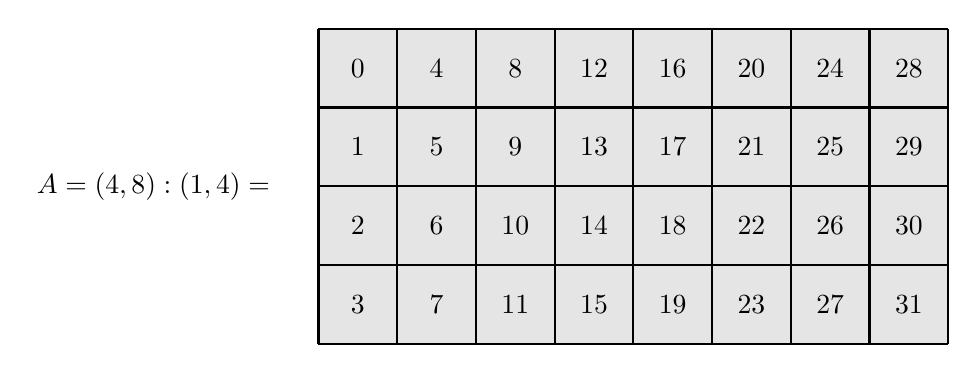
\begin{tikzpicture}[x={(0cm,-1cm)},y={(1cm,0cm)},every node/.style={minimum size=1cm, outer sep=0pt}]

\node[fill=gray!20] at (0,0) {0};
\node[fill=gray!20] at (0,1) {4};
\node[fill=gray!20] at (0,2) {8};
\node[fill=gray!20] at (0,3) {12};
\node[fill=gray!20] at (0,4) {16};
\node[fill=gray!20] at (0,5) {20};
\node[fill=gray!20] at (0,6) {24};
\node[fill=gray!20] at (0,7) {28};
\node[fill=gray!20] at (1,0) {1};
\node[fill=gray!20] at (1,1) {5};
\node[fill=gray!20] at (1,2) {9};
\node[fill=gray!20] at (1,3) {13};
\node[fill=gray!20] at (1,4) {17};
\node[fill=gray!20] at (1,5) {21};
\node[fill=gray!20] at (1,6) {25};
\node[fill=gray!20] at (1,7) {29};
\node[fill=gray!20] at (2,0) {2};
\node[fill=gray!20] at (2,1) {6};
\node[fill=gray!20] at (2,2) {10};
\node[fill=gray!20] at (2,3) {14};
\node[fill=gray!20] at (2,4) {18};
\node[fill=gray!20] at (2,5) {22};
\node[fill=gray!20] at (2,6) {26};
\node[fill=gray!20] at (2,7) {30};
\node[fill=gray!20] at (3,0) {3};
\node[fill=gray!20] at (3,1) {7};
\node[fill=gray!20] at (3,2) {11};
\node[fill=gray!20] at (3,3) {15};
\node[fill=gray!20] at (3,4) {19};
\node[fill=gray!20] at (3,5) {23};
\node[fill=gray!20] at (3,6) {27};
\node[fill=gray!20] at (3,7) {31};
\draw[color=black,thick,shift={(-0.5,-0.5)}] (0,0) grid (4,8);

\node[anchor=east] at (1.5,-1) {$A = (4,8):(1,4) = $};
\end{tikzpicture}

\end{centering} 

\bigskip

\noindent 出于各种目的，我们可能希望对布局 $A$ 进行{\it 铺砌}（tile）。例如，下面给出了用几种不同布局 $B$ 对 $A$ 所作的铺砌（tiling）。

\bigskip


\begin{centering}

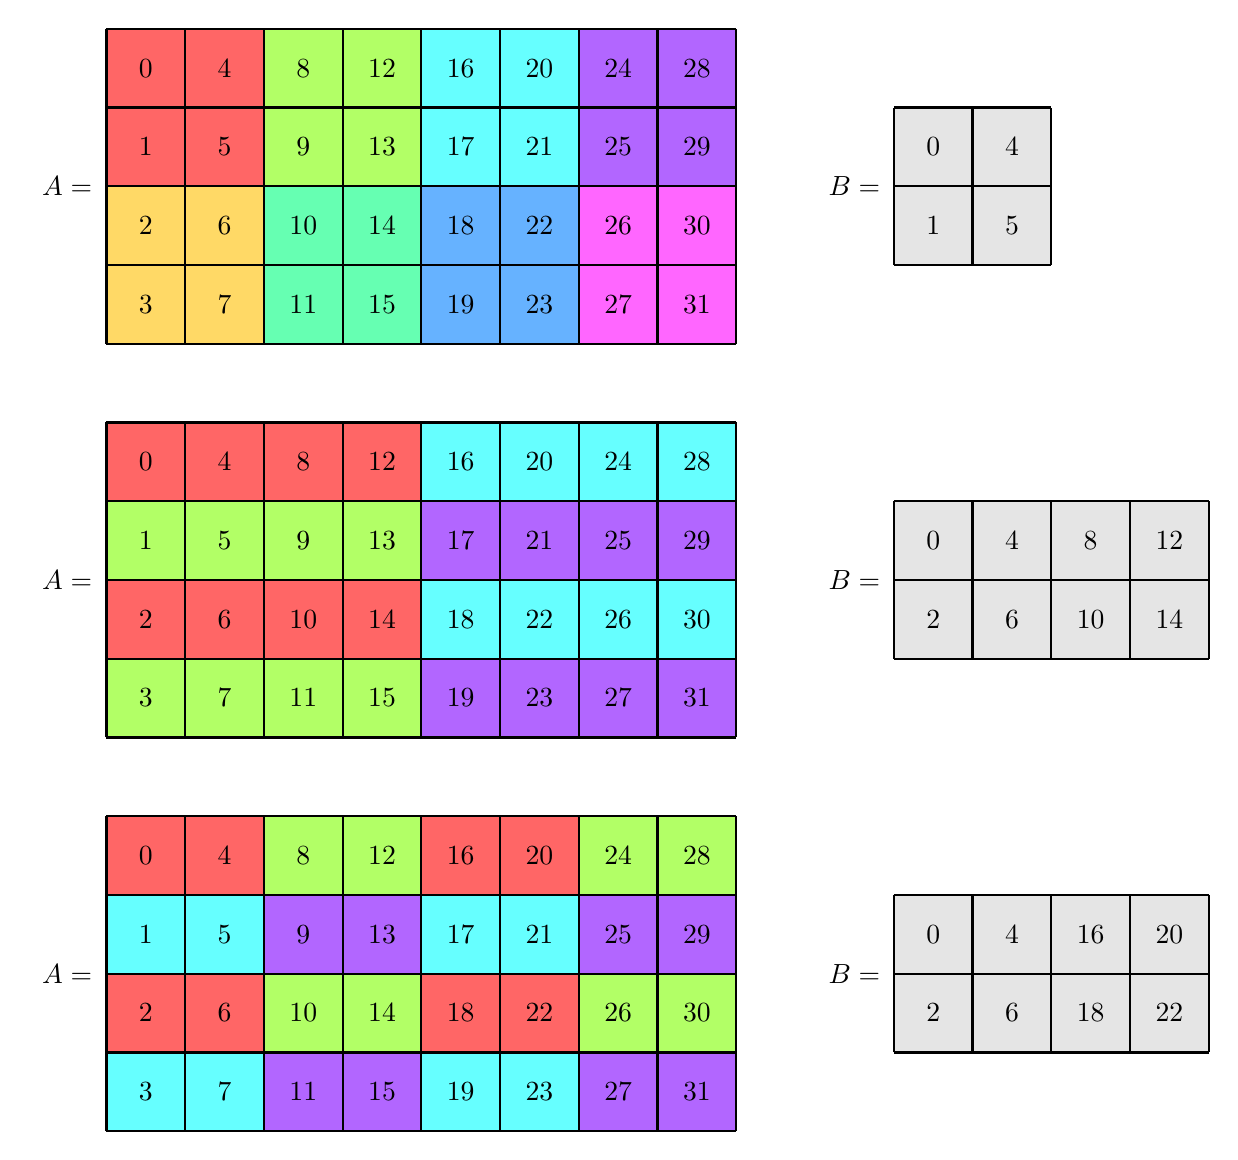
\begin{tikzpicture}[x={(0cm,-1cm)},y={(1cm,0cm)},every node/.style={minimum size=1cm, outer sep=0pt}]

\node[fill=colorx1!60] at (0,0) {0};
\node[fill=colorx1!60] at (0,1) {4};
\node[fill=colorx3!60] at (0,2) {8};
\node[fill=colorx3!60] at (0,3) {12};
\node[fill=colorx5!60] at (0,4) {16};
\node[fill=colorx5!60] at (0,5) {20};
\node[fill=colorx7!60] at (0,6) {24};
\node[fill=colorx7!60] at (0,7) {28};
\node[fill=colorx1!60] at (1,0) {1};
\node[fill=colorx1!60] at (1,1) {5};
\node[fill=colorx3!60] at (1,2) {9};
\node[fill=colorx3!60] at (1,3) {13};
\node[fill=colorx5!60] at (1,4) {17};
\node[fill=colorx5!60] at (1,5) {21};
\node[fill=colorx7!60] at (1,6) {25};
\node[fill=colorx7!60] at (1,7) {29};
\node[fill=colorx2!60] at (2,0) {2};
\node[fill=colorx2!60] at (2,1) {6};
\node[fill=colorx4!60] at (2,2) {10};
\node[fill=colorx4!60] at (2,3) {14};
\node[fill=colorx6!60] at (2,4) {18};
\node[fill=colorx6!60] at (2,5) {22};
\node[fill=colorx8!60] at (2,6) {26};
\node[fill=colorx8!60] at (2,7) {30};
\node[fill=colorx2!60] at (3,0) {3};
\node[fill=colorx2!60] at (3,1) {7};
\node[fill=colorx4!60] at (3,2) {11};
\node[fill=colorx4!60] at (3,3) {15};
\node[fill=colorx6!60] at (3,4) {19};
\node[fill=colorx6!60] at (3,5) {23};
\node[fill=colorx8!60] at (3,6) {27};
\node[fill=colorx8!60] at (3,7) {31};
\draw[color=black,thick,shift={(-0.5,-0.5)}] (0,0) grid (4,8);

\node at (1.5,-1) {$A = $};
\node at (1.5,9) {$B = $};

\node[fill=gray!20] at (1,10) {0};
\node[fill=gray!20] at (2,10) {1};
\node[fill=gray!20] at (1,11) {4};
\node[fill=gray!20] at (2,11) {5};
\draw[color=black,thick,shift={(-0.5,-0.5)}] (1,10) grid (3,12);

\node[fill=colorx1!60] at (5,0) {0};
\node[fill=colorx1!60] at (5,1) {4};
\node[fill=colorx1!60] at (5,2) {8};
\node[fill=colorx1!60] at (5,3) {12};
\node[fill=colorx5!60] at (5,4) {16};
\node[fill=colorx5!60] at (5,5) {20};
\node[fill=colorx5!60] at (5,6) {24};
\node[fill=colorx5!60] at (5,7) {28};
\node[fill=colorx3!60] at (6,0) {1};
\node[fill=colorx3!60] at (6,1) {5};
\node[fill=colorx3!60] at (6,2) {9};
\node[fill=colorx3!60] at (6,3) {13};
\node[fill=colorx7!60] at (6,4) {17};
\node[fill=colorx7!60] at (6,5) {21};
\node[fill=colorx7!60] at (6,6) {25};
\node[fill=colorx7!60] at (6,7) {29};
\node[fill=colorx1!60] at (7,0) {2};
\node[fill=colorx1!60] at (7,1) {6};
\node[fill=colorx1!60] at (7,2) {10};
\node[fill=colorx1!60] at (7,3) {14};
\node[fill=colorx5!60] at (7,4) {18};
\node[fill=colorx5!60] at (7,5) {22};
\node[fill=colorx5!60] at (7,6) {26};
\node[fill=colorx5!60] at (7,7) {30};
\node[fill=colorx3!60] at (8,0) {3};
\node[fill=colorx3!60] at (8,1) {7};
\node[fill=colorx3!60] at (8,2) {11};
\node[fill=colorx3!60] at (8,3) {15};
\node[fill=colorx7!60] at (8,4) {19};
\node[fill=colorx7!60] at (8,5) {23};
\node[fill=colorx7!60] at (8,6) {27};
\node[fill=colorx7!60] at (8,7) {31};
\draw[color=black,thick,shift={(-0.5,-0.5)}] (5,0) grid (9,8);

\node at (6.5,-1) {$A = $};
\node at (6.5,9) {$B = $};

\node[fill=gray!20] at (6,10) {0};
\node[fill=gray!20] at (7,10) {2};
\node[fill=gray!20] at (6,11) {4};
\node[fill=gray!20] at (7,11) {6};
\node[fill=gray!20] at (6,12) {8};
\node[fill=gray!20] at (7,12) {10};
\node[fill=gray!20] at (6,13) {12};
\node[fill=gray!20] at (7,13) {14};
\draw[color=black,thick,shift={(-0.5,-0.5)}] (6,10) grid (8,14);

\node[fill=colorx1!60] at (10,0) {0};
\node[fill=colorx1!60] at (10,1) {4};
\node[fill=colorx3!60] at (10,2) {8};
\node[fill=colorx3!60] at (10,3) {12};
\node[fill=colorx1!60] at (10,4) {16};
\node[fill=colorx1!60] at (10,5) {20};
\node[fill=colorx3!60] at (10,6) {24};
\node[fill=colorx3!60] at (10,7) {28};
\node[fill=colorx5!60] at (11,0) {1};
\node[fill=colorx5!60] at (11,1) {5};
\node[fill=colorx7!60] at (11,2) {9};
\node[fill=colorx7!60] at (11,3) {13};
\node[fill=colorx5!60] at (11,4) {17};
\node[fill=colorx5!60] at (11,5) {21};
\node[fill=colorx7!60] at (11,6) {25};
\node[fill=colorx7!60] at (11,7) {29};
\node[fill=colorx1!60] at (12,0) {2};
\node[fill=colorx1!60] at (12,1) {6};
\node[fill=colorx3!60] at (12,2) {10};
\node[fill=colorx3!60] at (12,3) {14};
\node[fill=colorx1!60] at (12,4) {18};
\node[fill=colorx1!60] at (12,5) {22};
\node[fill=colorx3!60] at (12,6) {26};
\node[fill=colorx3!60] at (12,7) {30};
\node[fill=colorx5!60] at (13,0) {3};
\node[fill=colorx5!60] at (13,1) {7};
\node[fill=colorx7!60] at (13,2) {11};
\node[fill=colorx7!60] at (13,3) {15};
\node[fill=colorx5!60] at (13,4) {19};
\node[fill=colorx5!60] at (13,5) {23};
\node[fill=colorx7!60] at (13,6) {27};
\node[fill=colorx7!60] at (13,7) {31};
\draw[color=black,thick,shift={(-0.5,-0.5)}] (10,0) grid (14,8);

\node at (11.5,-1) {$A = $};
\node at (11.5,9) {$B = $};

\node[fill=gray!20] at (11,10) {0};
\node[fill=gray!20] at (12,10) {2};
\node[fill=gray!20] at (11,11) {4};
\node[fill=gray!20] at (12,11) {6};
\node[fill=gray!20] at (11,12) {16};
\node[fill=gray!20] at (12,12) {18};
\node[fill=gray!20] at (11,13) {20};
\node[fill=gray!20] at (12,13) {22};
\draw[color=black,thick,shift={(-0.5,-0.5)}] (11,10) grid (13,14);
\end{tikzpicture}

\end{centering}


\bigskip 

在处理这类经过铺砌的布局时，我们希望能够用形如 $(\texttt{tile}\_\texttt{coordinate},\texttt{tile})$ 的坐标对布局进行索引，其中 $\texttt{tile}$ 指明我们正在操作的是哪一个瓦片（tile），而 $\texttt{tile}\_\texttt{coordinate}$ 指明所给瓦片内部的一个坐标。例如，若 $A$ 与 $B$ 的秩（rank）均为 $2$，我们便希望把 $((i,j),(k,\ell))$ 写作 $A$ 的第 $(k,\ell)$ 个瓦片中第 $(i,j)$ 个元素（entry）的索引。逻辑切分 $A \oslash B$ 正是为我们提供这一能力的布局。



\begin{definition}\label{definitionoflogicaldivide}
设 $A$ 与 $B$ 为布局，并设
\[B^c = \comp(B,\size(A))\]
为 $B$ 关于 $\size(A)$ 的补（complement）。则 $A$ 除以 $B$ 的{\it 逻辑切分}是布局
\begin{align*}
A \oslash B & = A \circ (B,B^c)\\
& = (A \circ B, A \circ B^c).
\end{align*}
\end{definition}


\begin{example}
    若 $A = (4,8):(1,4)$ 且 $B = (2,2):(1,4)$，则
    \[A \oslash B = ((2,2),(2,4)):((1,4),(2,8)),\]
    如下图所示。

    \bigskip


\begin{centering}
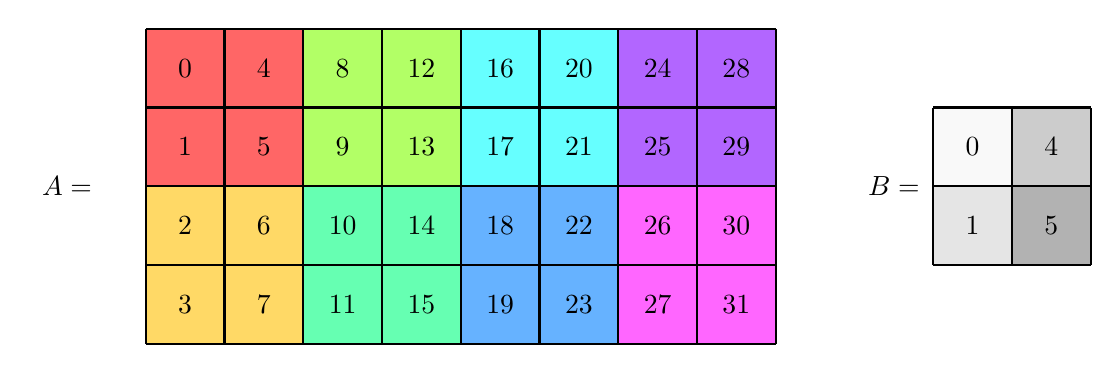
\begin{tikzpicture}[x={(0cm,-1cm)},y={(1cm,0cm)},every node/.style={minimum size=1cm, outer sep=0pt}]

\node[fill=colorx1!60] at (0,0) {0};
\node[fill=colorx1!60] at (0,1) {4};
\node[fill=colorx3!60] at (0,2) {8};
\node[fill=colorx3!60] at (0,3) {12};
\node[fill=colorx5!60] at (0,4) {16};
\node[fill=colorx5!60] at (0,5) {20};
\node[fill=colorx7!60] at (0,6) {24};
\node[fill=colorx7!60] at (0,7) {28};
\node[fill=colorx1!60] at (1,0) {1};
\node[fill=colorx1!60] at (1,1) {5};
\node[fill=colorx3!60] at (1,2) {9};
\node[fill=colorx3!60] at (1,3) {13};
\node[fill=colorx5!60] at (1,4) {17};
\node[fill=colorx5!60] at (1,5) {21};
\node[fill=colorx7!60] at (1,6) {25};
\node[fill=colorx7!60] at (1,7) {29};
\node[fill=colorx2!60] at (2,0) {2};
\node[fill=colorx2!60] at (2,1) {6};
\node[fill=colorx4!60] at (2,2) {10};
\node[fill=colorx4!60] at (2,3) {14};
\node[fill=colorx6!60] at (2,4) {18};
\node[fill=colorx6!60] at (2,5) {22};
\node[fill=colorx8!60] at (2,6) {26};
\node[fill=colorx8!60] at (2,7) {30};
\node[fill=colorx2!60] at (3,0) {3};
\node[fill=colorx2!60] at (3,1) {7};
\node[fill=colorx4!60] at (3,2) {11};
\node[fill=colorx4!60] at (3,3) {15};
\node[fill=colorx6!60] at (3,4) {19};
\node[fill=colorx6!60] at (3,5) {23};
\node[fill=colorx8!60] at (3,6) {27};
\node[fill=colorx8!60] at (3,7) {31};
\draw[color=black,thick,shift={(-0.5,-0.5)}] (0,0) grid (4,8);

\node[anchor = east] at (1.5,-1) {$A = $};
\node[anchor = east] at (1.5,9.5) {$B = $};

\node[fill=gray!5] at (1,10) {0};
\node[fill=gray!20] at (2,10) {1};
\node[fill=gray!40] at (1,11) {4};
\node[fill=gray!60] at (2,11) {5};
\draw[color=black,thick,shift={(-0.5,-0.5)}] (1,10) grid (3,12);
\end{tikzpicture}

\end{centering}

\vspace{0.2in}

\begin{centering}
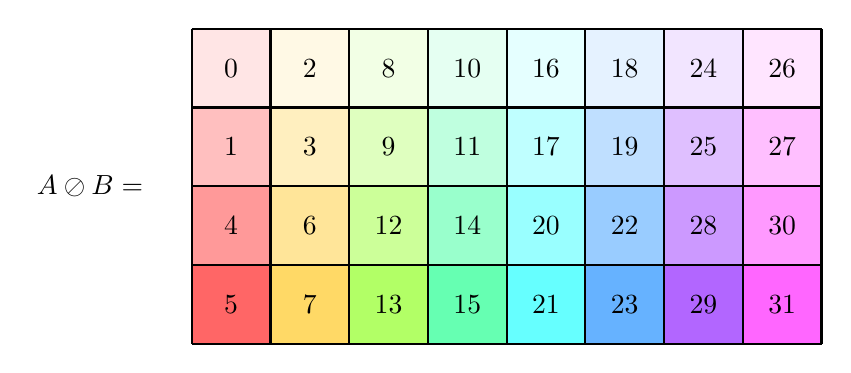
\begin{tikzpicture}[x={(0cm,-1cm)},y={(1cm,0cm)},every node/.style={minimum size=1cm, outer sep=0pt}]

\node[fill=colorx1!10]       at (0,0) {0};
\node[fill=colorx2!10]       at (0,1) {2};
\node[fill=colorx3!10]      at (0,2) {8};
\node[fill=colorx4!10]      at (0,3) {10};
\node[fill=colorx5!10]  at (0,4) {16};
\node[fill=colorx6!10]  at (0,5) {18};
\node[fill=colorx7!10]        at (0,6) {24};
\node[fill=colorx8!10]        at (0,7) {26};

\node[fill=colorx1!25]       at (1,0) {1};
\node[fill=colorx2!25]       at (1,1) {3};
\node[fill=colorx3!25]      at (1,2) {9};
\node[fill=colorx4!25]      at (1,3) {11};
\node[fill=colorx5!25]  at (1,4) {17};
\node[fill=colorx6!25]  at (1,5) {19};
\node[fill=colorx7!25]        at (1,6) {25};
\node[fill=colorx8!25]        at (1,7) {27};

\node[fill=colorx1!40]       at (2,0) {4};
\node[fill=colorx2!40]       at (2,1) {6};
\node[fill=colorx3!40]      at (2,2) {12};
\node[fill=colorx4!40]      at (2,3) {14};
\node[fill=colorx5!40]  at (2,4) {20};
\node[fill=colorx6!40]  at (2,5) {22};
\node[fill=colorx7!40]        at (2,6) {28};
\node[fill=colorx8!40]        at (2,7) {30};

\node[fill=colorx1!60]       at (3,0) {5};
\node[fill=colorx2!60]       at (3,1) {7};
\node[fill=colorx3!60]      at (3,2) {13};
\node[fill=colorx4!60]      at (3,3) {15};
\node[fill=colorx5!60]  at (3,4) {21};
\node[fill=colorx6!60]  at (3,5) {23};
\node[fill=colorx7!60]       at (3,6) {29};
\node[fill=colorx8!60]       at (3,7) {31};
\draw[color=black,thick,shift={(-0.5,-0.5)}] (0,0) grid (4,8);

\node[anchor=east] at (1.5,-1) {$ A \oslash B = $};

\end{tikzpicture}

\end{centering}
\end{example}

\begin{remark}
    $A \oslash B$ 中每个元素的{\it 颜色}（color）表明它属于哪个瓦片，而 $A\oslash B$ 中每个元素的{\it 不透明度}（opacity）表明它代表该瓦片中的哪个元素。这正是 $A\oslash B$ 的每一列颜色相同、每一行不透明度相同的原因。
\end{remark}


\begin{example}
    若 $A = (4,8):(1,4)$ 且 $B = (2,2):(4,1)$，则
    \[A \oslash B = ((2,2),(2,4)):((4,1),(2,8)),\]
    如下图所示。

    \bigskip


\begin{centering}
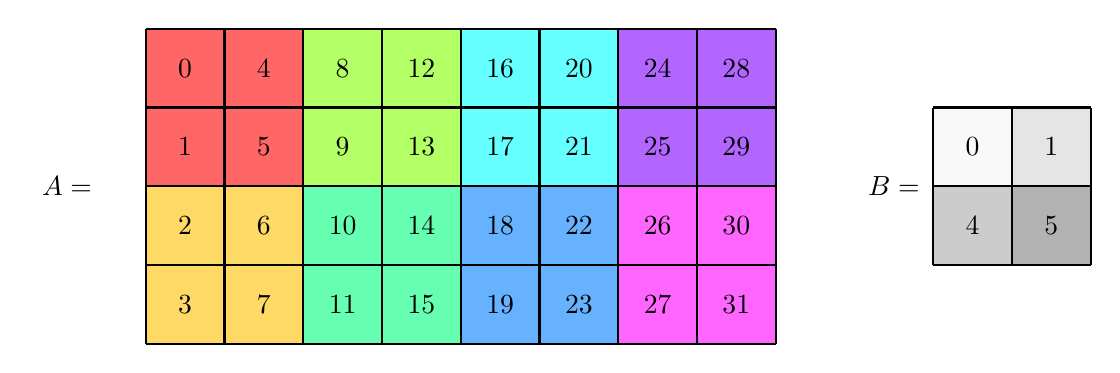
\begin{tikzpicture}[x={(0cm,-1cm)},y={(1cm,0cm)},every node/.style={minimum size=1cm, outer sep=0pt}]

\node[fill=colorx1!60] at (0,0) {0};
\node[fill=colorx1!60] at (0,1) {4};
\node[fill=colorx3!60] at (0,2) {8};
\node[fill=colorx3!60] at (0,3) {12};
\node[fill=colorx5!60] at (0,4) {16};
\node[fill=colorx5!60] at (0,5) {20};
\node[fill=colorx7!60] at (0,6) {24};
\node[fill=colorx7!60] at (0,7) {28};
\node[fill=colorx1!60] at (1,0) {1};
\node[fill=colorx1!60] at (1,1) {5};
\node[fill=colorx3!60] at (1,2) {9};
\node[fill=colorx3!60] at (1,3) {13};
\node[fill=colorx5!60] at (1,4) {17};
\node[fill=colorx5!60] at (1,5) {21};
\node[fill=colorx7!60] at (1,6) {25};
\node[fill=colorx7!60] at (1,7) {29};
\node[fill=colorx2!60] at (2,0) {2};
\node[fill=colorx2!60] at (2,1) {6};
\node[fill=colorx4!60] at (2,2) {10};
\node[fill=colorx4!60] at (2,3) {14};
\node[fill=colorx6!60] at (2,4) {18};
\node[fill=colorx6!60] at (2,5) {22};
\node[fill=colorx8!60] at (2,6) {26};
\node[fill=colorx8!60] at (2,7) {30};
\node[fill=colorx2!60] at (3,0) {3};
\node[fill=colorx2!60] at (3,1) {7};
\node[fill=colorx4!60] at (3,2) {11};
\node[fill=colorx4!60] at (3,3) {15};
\node[fill=colorx6!60] at (3,4) {19};
\node[fill=colorx6!60] at (3,5) {23};
\node[fill=colorx8!60] at (3,6) {27};
\node[fill=colorx8!60] at (3,7) {31};
\draw[color=black,thick,shift={(-0.5,-0.5)}] (0,0) grid (4,8);

\node[anchor = east] at (1.5,-1) {$A = $};
\node[anchor = east] at (1.5,9.5) {$B = $};

\node[fill=gray!5] at (1,10) {0};
\node[fill=gray!40] at (2,10) {4};
\node[fill=gray!20] at (1,11) {1};
\node[fill=gray!60] at (2,11) {5};
\draw[color=black,thick,shift={(-0.5,-0.5)}] (1,10) grid (3,12);
\end{tikzpicture}

\end{centering}

\vspace{0.2in}

\begin{centering}
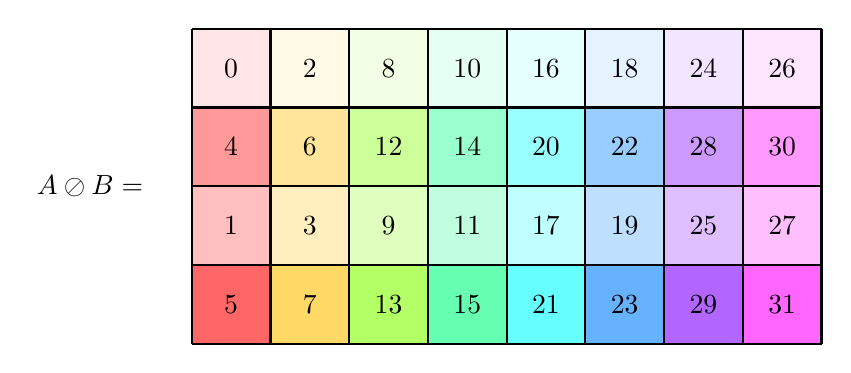
\begin{tikzpicture}[x={(0cm,-1cm)},y={(1cm,0cm)},every node/.style={minimum size=1cm, outer sep=0pt}]

\node[fill=colorx1!10] at (0,0) {0};
\node[fill=colorx2!10] at (0,1) {2};
\node[fill=colorx3!10] at (0,2) {8};
\node[fill=colorx4!10] at (0,3) {10};
\node[fill=colorx5!10] at (0,4) {16};
\node[fill=colorx6!10] at (0,5) {18};
\node[fill=colorx7!10] at (0,6) {24};
\node[fill=colorx8!10] at (0,7) {26};
\node[fill=colorx1!40] at (1,0) {4};
\node[fill=colorx2!40] at (1,1) {6};
\node[fill=colorx3!40] at (1,2) {12};
\node[fill=colorx4!40] at (1,3) {14};
\node[fill=colorx5!40] at (1,4) {20};
\node[fill=colorx6!40] at (1,5) {22};
\node[fill=colorx7!40] at (1,6) {28};
\node[fill=colorx8!40] at (1,7) {30};
\node[fill=colorx1!25] at (2,0) {1};
\node[fill=colorx2!25] at (2,1) {3};
\node[fill=colorx3!25] at (2,2) {9};
\node[fill=colorx4!25] at (2,3) {11};
\node[fill=colorx5!25] at (2,4) {17};
\node[fill=colorx6!25] at (2,5) {19};
\node[fill=colorx7!25] at (2,6) {25};
\node[fill=colorx8!25] at (2,7) {27};
\node[fill=colorx1!60] at (3,0) {5};
\node[fill=colorx2!60] at (3,1) {7};
\node[fill=colorx3!60] at (3,2) {13};
\node[fill=colorx4!60] at (3,3) {15};
\node[fill=colorx5!60] at (3,4) {21};
\node[fill=colorx6!60] at (3,5) {23};
\node[fill=colorx7!60] at (3,6) {29};
\node[fill=colorx8!60] at (3,7) {31};
\draw[color=black,thick,shift={(-0.5,-0.5)}] (0,0) grid (4,8);



\node[anchor=east] at (1.5,-1) {$ A \oslash B = $};

% \node at (0,-1) {\Large{\texttt{0}}};
% \node at (1,-1) {\Large{\texttt{1}}};
% \node at (2,-1) {\Large{\texttt{2}}};
% \node at (3,-1) {\Large{\texttt{3}}};
% \node at (-1,0) {\Large{\texttt{0}}};
% \node at (-1,1) {\Large{\texttt{1}}};
% \node at (-1,2) {\Large{\texttt{2}}};
% \node at (-1,3) {\Large{\texttt{3}}};
% \node at (-1,4) {\Large{\texttt{4}}};
% \node at (-1,5) {\Large{\texttt{5}}};
% \node at (-1,6) {\Large{\texttt{6}}};
% \node at (-1,7) {\Large{\texttt{7}}};
\end{tikzpicture}

\end{centering}
\end{example}


\begin{remark}
    注意前两个例子之间的差别。两个例子中对 $A$ 的铺砌完全相同，但每个瓦片内部的布局各不相同。在第一个例子中，各瓦片具有列主序（column-major）布局，而在第二个例子中，各瓦片具有行主序（row-major）布局。这导致进行逻辑切分时得到不同的布局。
\end{remark}














\begin{example}
    若 $A = (4,8):(1,4)$ 且 $B = (2,4):(2,4)$，则
    \[A \oslash B = ((2,4),(2,2)):((2,4),(1,16)).\]
\end{example}


\begin{example}
    若 $A = (4,6):(1,40)$ 且 $B = 6:4$，则
    \[
    A \oslash B = (6,4):(40,1).
    \]
\end{example}

\begin{example}
    若 $A = (4,6,2,4,2,5) : (36,1,18,0,0,144 )$ 且 $B = (4,10):(1,192)$，则
    \[
    A \oslash B = (((4,(2,5)),(6,2,4)):((36,(0,144)
    ),(1,18,0))
    \]
\end{example}

\begin{example}
    若 $A = (8,(4,4))$ 且 $B = (2,(8,16))$，则
    \[
    A \oslash B = ((2,2),(2,(4,4))):((4,8),(2,(8,16))).
    \]
\end{example}

\subsection{逻辑乘积}\label{logicalproductsection}

本节定义布局的{\bf 逻辑乘积}（logical product）。
% For example, consider the layouts 

%     \[
%     \begin{tikzpicture}[x={(0cm,-1cm)},y={(1cm,0cm)},every node/.style={minimum size=1cm, outer sep=0pt}]

% \node[fill=colorx2!60] at (0,0) {0};
% \node[fill=colorx4!60] at (0,1) {1};
% \node[fill=colorx6!60] at (1,0) {2};
% \node[fill=colorx8!60] at (1,1) {3};
% \draw[color=black,thick,shift={(-0.5,-0.5)}] (0,0) grid (2,2);

% \node[fill=gray!20] at (0,5) {0};
% \node[fill=gray!20] at (0,6) {0};
% \node[fill=gray!20] at (0,7) {0};
% \node[fill=gray!20] at (1,5) {0};
% \node[fill=gray!20] at (1,6) {0};
% \node[fill=gray!20] at (1,7) {0};
% \draw[color=black,thick,shift={(-0.5,-0.5)}] (0,5) grid (2,8);

% \node[anchor = east] at (0.5,-1) {$A = $ };
% \node[anchor = east] at (0.5,4) {$B = $ };

% \end{tikzpicture}
%     \]

\begin{definition} \label{definitionoflogicalproduct}
设 $A$ 与 $B$ 为布局，并设
\[
A^c = \comp\bigl(A,\size(A)\cdot \cosize(B) \bigr)
\]
为 $A$ 关于 $\size(A) \cdot \cosize(B)$ 的补。则 $A$ 与 $B$ 的{\it 逻辑乘积}是布局
\[
A \otimes B = (A , A^c \circ B).
\]
\end{definition}

\begin{observation}
    由命题 \ref{postcomposewithextension} 与命题 \ref{postcomposewithcoalesce} 可知，若对任意合法的 $N \geq \size(A) \cdot \cosize(B)$ 令
    \[
    \widetilde{A}^c = \comp(A,N)
    \]
    则有
    \[
    A^c \circ B = \tilde{A}^c \circ B.
    \]
    这意味着在计算 $A \otimes B$ 时，可以把 $A^c$ 取为 $A$ 的任意足够大的（已排序的）补。
\end{observation}

\begin{example}
    若 $A = (2,2):(5,10)$ 与 $B = (3,5):(5,1)$ 为布局
    \[
    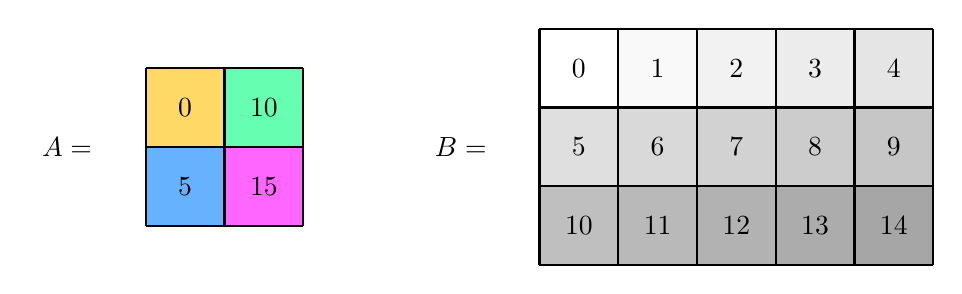
\begin{tikzpicture}[x={(0cm,-1cm)},y={(1cm,0cm)},every node/.style={minimum size=1cm, outer sep=0pt}]

\node[fill=colorx2!60] at (0.5,0) {0};
\node[fill=colorx4!60] at (0.5,1) {10};
\node[fill=colorx6!60] at (1.5,0) {5};
\node[fill=colorx8!60] at (1.5,1) {15};
\draw[color=black,thick,shift={(0,-0.5)}] (0,0) grid (2,2);

\node[fill=gray!0] at (0,5) {0};
\node[fill=gray!5] at (0,6) {1};
\node[fill=gray!10] at (0,7) {2};
\node[fill=gray!15] at (0,8) {3};
\node[fill=gray!20] at (0,9) {4};
\node[fill=gray!25] at (1,5) {5};
\node[fill=gray!30] at (1,6) {6};
\node[fill=gray!35] at (1,7) {7};
\node[fill=gray!40] at (1,8) {8};
\node[fill=gray!45] at (1,9) {9};
\node[fill=gray!50] at (2,5) {10};
\node[fill=gray!55] at (2,6) {11};
\node[fill=gray!60] at (2,7) {12};
\node[fill=gray!65] at (2,8) {13};
\node[fill=gray!70] at (2,9) {14};
\draw[color=black,thick,shift={(-0.5,-0.5)}] (0,5) grid (3,10);

\node[anchor = east] at (1,-1) {$A = $ };
\node[anchor = east] at (1,4) {$B = $ };

\end{tikzpicture}
    \]
    则 $A \otimes B$ 为布局
    \[
    A \otimes B = ((2,2),(3,5)):((5,10),(20,1))
    \]
如下图所示。
    
\[
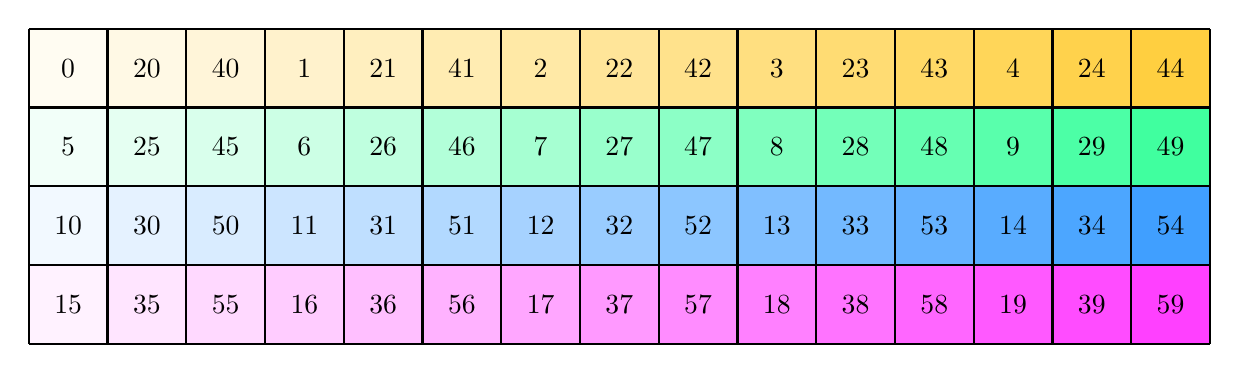
\begin{tikzpicture}[x={(0cm,-1cm)},y={(1cm,0cm)},every node/.style={minimum size=1cm, outer sep=0pt}]
\node[fill=colorx2!5] at (0,0) {0};
\node[fill=colorx2!10] at (0,1) {20};
\node[fill=colorx2!15] at (0,2) {40};
\node[fill=colorx2!20] at (0,3) {1};
\node[fill=colorx2!25] at (0,4) {21};
\node[fill=colorx2!30] at (0,5) {41};
\node[fill=colorx2!35] at (0,6) {2};
\node[fill=colorx2!40] at (0,7) {22};
\node[fill=colorx2!45] at (0,8) {42};
\node[fill=colorx2!50] at (0,9) {3};
\node[fill=colorx2!55] at (0,10) {23};
\node[fill=colorx2!60] at (0,11) {43};
\node[fill=colorx2!65] at (0,12) {4};
\node[fill=colorx2!70] at (0,13) {24};
\node[fill=colorx2!75] at (0,14) {44};
\node[fill=colorx4!5] at (1,0) {5};
\node[fill=colorx4!10] at (1,1) {25};
\node[fill=colorx4!15] at (1,2) {45};
\node[fill=colorx4!20] at (1,3) {6};
\node[fill=colorx4!25] at (1,4) {26};
\node[fill=colorx4!30] at (1,5) {46};
\node[fill=colorx4!35] at (1,6) {7};
\node[fill=colorx4!40] at (1,7) {27};
\node[fill=colorx4!45] at (1,8) {47};
\node[fill=colorx4!50] at (1,9) {8};
\node[fill=colorx4!55] at (1,10) {28};
\node[fill=colorx4!60] at (1,11) {48};
\node[fill=colorx4!65] at (1,12) {9};
\node[fill=colorx4!70] at (1,13) {29};
\node[fill=colorx4!75] at (1,14) {49};
\node[fill=colorx6!5] at (2,0) {10};
\node[fill=colorx6!10] at (2,1) {30};
\node[fill=colorx6!15] at (2,2) {50};
\node[fill=colorx6!20] at (2,3) {11};
\node[fill=colorx6!25] at (2,4) {31};
\node[fill=colorx6!30] at (2,5) {51};
\node[fill=colorx6!35] at (2,6) {12};
\node[fill=colorx6!40] at (2,7) {32};
\node[fill=colorx6!45] at (2,8) {52};
\node[fill=colorx6!50] at (2,9) {13};
\node[fill=colorx6!55] at (2,10) {33};
\node[fill=colorx6!60] at (2,11) {53};
\node[fill=colorx6!65] at (2,12) {14};
\node[fill=colorx6!70] at (2,13) {34};
\node[fill=colorx6!75] at (2,14) {54};
\node[fill=colorx8!5] at (3,0) {15};
\node[fill=colorx8!10] at (3,1) {35};
\node[fill=colorx8!15] at (3,2) {55};
\node[fill=colorx8!20] at (3,3) {16};
\node[fill=colorx8!25] at (3,4) {36};
\node[fill=colorx8!30] at (3,5) {56};
\node[fill=colorx8!35] at (3,6) {17};
\node[fill=colorx8!40] at (3,7) {37};
\node[fill=colorx8!45] at (3,8) {57};
\node[fill=colorx8!50] at (3,9) {18};
\node[fill=colorx8!55] at (3,10) {38};
\node[fill=colorx8!60] at (3,11) {58};
\node[fill=colorx8!65] at (3,12) {19};
\node[fill=colorx8!70] at (3,13) {39};
\node[fill=colorx8!75] at (3,14) {59};
\draw[color=black,thick,shift={(-0.5,-0.5)}] (0,0) grid (4,15);
\end{tikzpicture}
\]
\end{example}

\begin{example} 若 $A = (3,3):(6,1)$ 且 $B = (10,12):(24,2)$，则
    \[ 
    A \otimes B = \bigl((3,3),(10,12) \bigr) : \bigl((6,1),(216,18) \bigr).
    \]
\end{example}

\begin{example}
    若 $A = (2,10):(1680,4) $ 且 $B = (4,9):(2,56)$，则
    \[
    A \otimes B = ( (2,10) , ((2,2),(3,3) ) ) : ((1680,4), ( ( 2 ,40 ) , (560,3360 )  ) ).
    \]
\end{example}

\begin{example}
    若 $A = (4,(2,2)):(9,(1,3))$ 且 $B = ((2,4),8):((1,4),2)$，则
    \[
    A \otimes B = ( ( 4,(2,2)),((2,4),8 ) ) : ( ( 9,(1,3)),((36,144),72 ) ).
    \]
\end{example}

\subsection{可处理布局}

本节定义一类性质特别良好的布局，称为{\it 可处理}（tractable）布局。我们将看到，可处理布局恰好是来自某个范畴（category）$\catstyle{Nest}$ 的布局。

\begin{definition}\label{definitionoftractablelayouts}
    我们称布局 $L$ 是{\it 可处理}的，如果扁平布局（flat layout）$L^\flat$ 依定义 \ref{definitionoftractableflatlayouts} 的意义是可处理的。确切地说，$L$ 是可处理的，如果扁平布局
    \[
    \sort(L^\flat) = (s_1,\dots,s_m):(d_1,\dots,d_m)
    \]
    满足：对每个 $1 \leq i < m$，有
    \begin{enumerate}
        \item $d_i = 0$\text{，或}
        \item $s_id_i$ 整除（divides）$d_{i+1}$。
    \end{enumerate}
\end{definition}

\begin{example}
    布局
    \[L = (((12))):(((17)))\]
    是可处理的。更一般地，任何长度为 $1$ 的布局 $L$ 都是可处理的。
\end{example}

\begin{example}
    布局
    \[L = ((2,4),32):((1,2),8)\]
    是可处理的。更一般地，任何列主序布局都是可处理的。
\end{example}
\begin{example}
    布局
    \[L = (2,(4,32)):(128,(32,1))\]
    是可处理的。更一般地，任何行主序布局 $L$ 都是可处理的。
\end{example}
\begin{example}
    布局
    \[L = ((3,3),(1,3),(3,1,3)):((81,1),(0,8),(3,0,27))\]
    是可处理的。更一般地，任何紧凑（compact）布局都是可处理的。
\end{example}

\begin{example}
    布局
    \[L = ((3,7,7)):((0,15,0))\]
    是可处理的。更一般地，任何恰有一个非零步长（stride）元素的布局都是可处理的。
\end{example}

\begin{example}
    布局
    \[L = (2,(2,(2,2))):(1,(2048,(16,64)))\]
    是可处理的。更一般地，任何可求补（complementable）布局都是可处理的。
\end{example}


\begin{example}
    布局
    \[L = ((8,8),(5,5)):((8,1),(10,2))\]
    不是可处理的。特别地，这表明可处理布局 $L_1$ 与 $L_2$ 的拼接（concatenation）$(L_1,L_2)$ 未必是可处理的。
\end{example}



% cf-ch3a.tex — 译自 FinalVersion.tex L6745-7835
\chapter{布局的范畴}\label{categorieschapter}

在深入探讨了布局的代数之后，我们现在把注意力转向本书的数学核心：把布局（layout）实现为适当定义的范畴（category）中的态射（morphism）。在此过程中，我们将发展一套\emph{布局图的图像演算}，它使布局运算的计算更为直接。

\section{范畴 $\catstyle{Tuple}$}\label{thecategoryTuplesection}

本节中，我们定义一个范畴 $\catstyle{Tuple}$，其对象（object）是正整数元组（tuple），其态射我们称为{\it 元组态射}（tuple morphism）。每个元组态射 $f:S \to T$ 编码一个扁平布局（flat layout）$L_f$。元组态射的复合（composition）与布局复合相容：若 $f$ 与 $g$ 是可复合的元组态射，则
\[
L_{g \circ f}= L_g \circ L_f.
\]
我们定义一个实现函子（realization functor）（\Cref{constructionofrealizationfunctoronC}）
\[
| \cdot |: \catstyle{Tuple} \to \catstyle{FinSet}
\]
它通过公式
\[
|f| = \Phi_{L_f}^{\size(T)}.
\]
恢复 $L_f$ 的布局函数（layout function）。我们还将发展一套「元组态射代数」，其中包括{\it 排序}（sort）（\Cref{subsubsection.sort}）、{\it 合并}（coalesce）（\Cref{subsubsection.coalesce}）、{\it 求补}（complement）（\Cref{subsubsection.complement}）、{\it 拼接}（concatenate）（\Cref{subsubsection.concatenate}）、{\it 扁平切分}（flat division）（\Cref{subsubsection.flatdivision}）与{\it 扁平乘积}（flat products）（\Cref{subsubsection.flatproduct}）等运算，它们与扁平布局上的相应运算相容。

\subsection{基本定义}



\begin{definition}
令 $\catstyle{Fin}_*$ 表示这样一个范畴：其对象是基点有限集（pointed finite set）
\[
\langle m \rangle_* = \{*,1,2,\dots,m\}
\]
其中 $m \geq 0$；其态射 $\alpha: \langle m \rangle_* \to \langle n \rangle_*$ 是满足 $\alpha(*) = *$ 的函数。我们称这类态射为{\it 基点映射}（pointed map），或简称{\it 映射}。
\end{definition}

\begin{aside}
    $\Fin_*$ 是由有限基点集构成的范畴 $\FinSet_*$ 的一个\emph{骨架}（skeleton）。
\end{aside}

\begin{notation} 若基点映射 $\alpha:\langle m \rangle_* \to \langle n \rangle_*$ 的陪域（codomain）已知，我们有时把 $\alpha$ 写成
\[
\alpha = (\alpha(1),\dots,\alpha(m))
\]
即一个长度为 $m$、元素（entry）取自 $\langle n \rangle_*$ 的元组。
\end{notation}
\begin{example}\label{morphisminFinexample1}
    在 $\catstyle{Fin}_*$ 中有一个态射 $\alpha : \langle 4 \rangle_* \to \langle 6 \rangle_*$，由
    \[
    \alpha = (2,1,*,6),
    \]
    给出，我们可以用下图来可视化它。
    \[ \begin{tikzcd} [row sep = 1, column sep = 8]
          & & \bullet \\
     & & \bullet \\
    \bullet \ar[uurr,mapsto] & & \bullet \\
    \bullet & & \bullet \\
    \bullet  \ar[drr,mapsto] & & \bullet \\
    \bullet\ar[urr,mapsto] & & \bullet \\
    & \alpha & \\
    \end{tikzcd} \]
    注意，与元素 $3$ 对应的圆点不带有箭头，这反映了它被送到 $*$ 这一事实。
\end{example}

\begin{example}\label{morphisminFinexample2}
    在 $\catstyle{Fin}_*$ 中有一个态射 $\beta:\langle 5 \rangle_* \to \langle 3 \rangle_*$，由
    \[
    \beta = (*,1,2,3,*)~,
    \]
    给出，我们可以用下图来可视化它。
    \[ \begin{tikzcd} [row sep = 1, column sep = 8]
    \bullet & & \\
    \bullet \ar[drr,mapsto]& & \\
    \bullet \ar[drr,mapsto]& & \bullet\\
    \bullet \ar[drr,bend left = 10, mapsto] & & \bullet\\
    \bullet \ar[rr,mapsto] & & \bullet\\
    & \beta & \\
    \end{tikzcd} \]
\end{example}

\begin{example}\label{morphisminFinexample3}
对任意 $m \geq 0$，$\catstyle{Fin}_*$ 中存在唯一形如 $\pi:\langle m \rangle_* \to \langle 0 \rangle_*$ 的态射，即
\[
\pi = (*,\dots,*).
\]
\end{example}

\begin{example}
对任意 $n \geq 0$，$\catstyle{Fin}_*$ 中存在唯一形如 $\delta : \langle 0 \rangle_* \to \langle m \rangle_*$ 的态射，即
    \[
    \delta = ().
    \]
\end{example}

\begin{aside}
    范畴 $\catstyle{Fin}_*$ 是交换 operad 的算子范畴（category of operators），因此我们有时记
    \[\catstyle{Fin}_* = \catstyle{Comm}^\otimes.\]
\end{aside}

\noindent 我们尤其关注 $\catstyle{Fin}_*$ 中的{\it 可处理}（tractable）态射，其定义如下。

\begin{definition}\label{definitionofessentiallyinjective}
    我们称基点映射 $\alpha: \langle m \rangle_* \to \langle n \rangle_*$ 是{\it 可处理的}，如果对任意 $j \in \langle n \rangle \subset \langle n \rangle_*$，原像（preimage）$\alpha^{-1}(j)$ 为空或由单个元素组成。
\end{definition}

\begin{example}\label{essentiallyinjectivemorphismexample}
    映射
    \[ \begin{tikzcd} [row sep = 1, column sep = 8]
            & &          & & & \bullet & &        & & & \bullet \ar[drr,mapsto] & & \bullet \\
            & &          & & & \bullet \ar[rr,mapsto] & & \bullet & & & \bullet \ar[urr,mapsto] & & \bullet \\
            & & \bullet   & & & \bullet \ar[drr,mapsto] & & \bullet & & & \bullet \ar[drr,mapsto] & & \bullet \\
    \bullet \ar[urr,mapsto] & & \bullet & & & \bullet & & \bullet & & & \bullet \ar[drr,mapsto]  & & \bullet \\
    \bullet \ar[rr,mapsto]& & \bullet & & & \bullet & & \bullet & & & \bullet \ar[uurr,mapsto] & & \bullet \\
    & \alpha_1 & & & & & \alpha_2 & & & & & \alpha_3 & & \\
    \end{tikzcd} \]
    是可处理的，而映射
    \[ \begin{tikzcd} [row sep = 1, column sep = 8]
    & &          & & & \bullet & &        & & & \bullet \ar[drr,mapsto] & & \bullet \\
    & &          & & & \bullet \ar[rr,mapsto] & & \bullet & & & \bullet \ar[urr,mapsto] & & \bullet \\
    & & \bullet   & & & \bullet \ar[drr,mapsto] & & \bullet & & & \bullet \ar[drr,bend left = 10, mapsto] & & \bullet \\
    \bullet \ar[drr,bend left = 10, mapsto] & & \bullet & & & \bullet & & \bullet & & & \bullet \ar[rr,mapsto]  & & \bullet \\
    \bullet \ar[rr,mapsto]& & \bullet & & & \bullet \ar[urr,mapsto] & & \bullet & & & \bullet \ar[urr,bend right = 10, mapsto] & & \bullet \\
    & \beta_1 & & & & & \beta_2 & & & & & \beta_3 & & \\
    \end{tikzcd} \]
    不是可处理的
\end{example}

\begin{remark}
    若我们把 $\catstyle{Fin}_*$ 中的态射 $\alpha:\langle m \rangle_* \to \langle n \rangle_*$ 表示为元组，即
    \[
    \alpha = (\alpha(1),\dots,\alpha(m))
    \]
    则 $\alpha$ 可处理当且仅当 $\alpha$ 中没有正整数出现多于一次。
\end{remark}

\begin{aside} 由可处理基点映射确定的宽子范畴（wide subcategory）
\[\catstyle{E}_0^\otimes \subset \catstyle{Comm}^\otimes = \catstyle{Fin}_*\]是 $\catstyle{E}_0$ operad 的算子范畴。
\end{aside}



\begin{definition}\label{definitionofTuple} 令 $\catstyle{Tuple}$ 表示这样一个范畴：其对象是正整数元组
\[
S = (s_1,\dots,s_m)
\]
其中的态射
\[f:(s_1,\dots,s_m) \to (t_1,\dots,t_n)\]
由一个可处理基点映射 $\alpha:\langle m \rangle_* \to \langle n \rangle_*$
指定，且满足以下性质：
\begin{itemize}
\item 若 $ 1 \leq i \leq m$ 且 $\alpha(i) \neq *$，则 $s_i = t_{\alpha(i)}$~。
\end{itemize}
我们称这样的态射 $f$ {\it 位于} $\alpha$ {\it 之上}（lies over），并把 $f$ 称为{\it 元组态射}。
\end{definition}

\begin{notation}
    若 $f:(s_1,\dots,s_m) \to (t_1,\dots,t_n)$ 是位于 $\alpha$ 之上的元组态射，我们有时把 $f$ 画成
    \[
    \begin{tikzcd}
(s_1,\dots,s_m) \ar[rr,"f"] \ar[rr,swap,"\alpha"] & & (t_1,\dots,t_n).
    \end{tikzcd}
    \]
\end{notation}

我们所发展的布局图像演算，基于 $\Tuple$ 中态射的自然可视化，如下例所示。

\begin{example}
\label{morphismfinC} 元组态射
\[
\begin{tikzcd}
(3,128,128) \ar[rr,"f"] \ar[rr,swap,"(1{,}3{,}5)"] & &  (3,2,128,2,128)
\end{tikzcd} \]
可以用下图来可视化。
    \[
    \begin{tikzcd}[row sep = 1, column sep = 8]
     & & 128  \\
     & & 2   \\
     128 \ar[rruu, mapsto] & & 128  \\
     128  \ar[rru,mapsto] & & 2  \\
     3 \ar[rr,mapsto] & & 3  \\
     & f &  \\
    \end{tikzcd}
    \]
    \end{example}


\begin{example}
\label{morphismginC}
元组态射
\[\begin{tikzcd}
(3,128,128) \ar[rr,"g"] \ar[rr,swap,"(*{,}2{,}1)"] & &  (128,128)
\end{tikzcd} \]
可以用下图来可视化。

\[
    \begin{tikzcd}[row sep = 1, column sep = 8]
     128 \ar[rrdd, mapsto] & &  \\
     128 \ar[rr,mapsto] & & 128 \\
     3 & & 128 \\
     & g & \\
    \end{tikzcd}
    \]
\end{example}
\begin{example}\label{morphismhinC}
    元组态射
    \[ \begin{tikzcd}
    (16,16,16,1,32) \ar[rr,"h"] \ar[rr,swap,"(*{,}*{,}1{,}*{,}2)"] & &  (16,32,1,1)
    \end{tikzcd} \]
    可以用下图来可视化。
    \[
    \begin{tikzcd} [row sep = 1, column sep = 8]
    32 \ar[dddrr,mapsto] & & \\
    1 & & 1 \\
    16 \ar[ddrr,mapsto] & & 1 \\
    16 & & 32 \\
    16 & & 16 \\
    & h & \\
    \end{tikzcd}
    \]
\end{example}

\begin{observation}
    我们可以如下把范畴 $\catstyle{Tuple}$ 与一些熟知的 operad 联系起来。令 $\mathbb{Z}_{>0}^{\mathterm{div}}$ 表示正整数依整除关系构成的偏序集（poset），并把它视为一个对称幺半范畴（symmetric monoidal category），其乘积由整数的乘法给出。令 $(\mathbb{Z}_{>0}^{\mathterm{div}})^\otimes$ 表示 $\mathbb{Z}_{>0}^{\mathterm{div}}$ 的算子范畴。于是存在显然的函子（functor）\[\catstyle{Tuple} \to (\mathbb{Z}_{>0}^{\mathterm{div}})^\otimes,\]与\[\catstyle{Tuple} \to \catstyle{E}_0^\otimes,\]使得图
    \[ \begin{tikzcd}
    \catstyle{Tuple} \ar[r] \ar[d] & (\mathbb{Z}_{>0}^{\mathterm{div}})^\otimes \ar[d] \\
    \catstyle{E}_0^\otimes \ar[r] & \catstyle{Comm}^\otimes
    \end{tikzcd} \]
    交换。这把 $\catstyle{Tuple}$ 展现为拉回（pullback）operad
    \[
    \catstyle{Tuple} \subset \catstyle{E}_0^\otimes \times_{\catstyle{Comm}^\otimes}(\mathbb{Z}_{>0}^{\mathterm{div}})^\otimes\]
    中由满足
    \[
    \alpha(i) \neq 1 \quad \Rightarrow \quad  s_i = t_{\alpha(i)}.
    \]
    的态射
    \[\begin{tikzcd} (s_1,\dots,s_m) \ar[r,"f"] \ar[r,swap,"\alpha"] & (t_1,\dots,t_n)
    \end{tikzcd}\]
    构成的宽子范畴。
\end{observation}

\subsection{从元组态射到扁平布局}

\noindent 使用范畴 $\Tuple$ 的动因在于：每个元组态射 $f$ 都编码一个扁平布局 $L_f$。而且，每个可处理布局 $L$ 都产生一个元组态射 $f_L$。我们在 \Cref{tractableflatlayoutscomefromtuplemorphisms} 中证明：这两个构造在某种意义上互为逆，且可处理布局恰是那些由元组态射编码的布局。

\begin{construction} \label{layoutfrommorphisminTuple}
设
\[\begin{tikzcd} (s_1,\dots,s_m) \ar[rr,"f"] \ar[rr,swap,"\alpha"] & &  (t_1,\dots,t_n)\end{tikzcd} \]
是一个元组态射。我们定义 $L_f$ 为这样一个扁平布局：其形状（shape）
\[\shape(L_f) = (s_1,\dots,s_m)\]
是 $f$ 的定义域（domain），其步长（stride）
\[\stride(L_f) = (d_1,\dots,d_m)\] 由公式
\[d_i = \begin{cases}
0 & \alpha(i) = * \\
\prod_{j < \alpha(i)} t_j & \alpha(i) \neq *.
\end{cases}
\]
定义。我们把 $L_f$ 称为 $f$ 所{\it 编码的布局}（layout encoded by $f$），或 $f$ 所\emph{关联的布局}（layout associated to $f$）。
\end{construction}




\begin{example} 例 \ref{morphismfinC} 中的元组态射
\[
\begin{tikzcd}[row sep = 1, column sep = 8]
 & & 128  \\
 & & 2   \\
 128 \ar[rruu, mapsto] & & 128  \\
 128  \ar[rru,mapsto] & & 2  \\
 3 \ar[rr,mapsto] & & 3  \\
 & f &  \\
\end{tikzcd}
\]
编码布局
\[
L_f  = (3,128,128) : (1,6,1536).
\]
注意，按 \Cref{layoutfrommorphisminTuple} 中的公式计算步长，相当于沿着从某个形状元素指向其目标元素的箭头，把该目标元素下方的所有元素相乘（空积取为 $1$）。
    % \[
    % \begin{tikzcd}[row sep = 1, column sep = 8]
    % & & & 128 & & & & &  \\
    % & & & 2 & & & & &  \\
    % & 128 \ar[rruu, mapsto] & & 128 & & & & & \\
    % & 128 \ar[rru,mapsto] & & 2 & & & \rightsquigarrow & & L_f = (3,128,128) : (1,6,1536)\\
    % & 3 \ar[rr,mapsto] & & 3 & & & & & \\
    % & & f & & & & & &  \\
    % \end{tikzcd}
    % \]
\end{example}

\begin{example} 例 \ref{morphismginC} 中的元组态射
\[\begin{tikzcd}
(3,128,128) \ar[rr,"g"] \ar[rr,swap,"(*{,}2{,}1)"] & &  (128,128)
\end{tikzcd} \]
编码布局
\[
L_g = (3,128,128):(0,128,1).
\]
% \[
%     \begin{tikzcd}[row sep = 1, column sep = 8]
%     & 128 \ar[rrdd, mapsto] & & & & & & & \\
%     & 128 \ar[rr,mapsto] & & 128 & & & \rightsquigarrow & & L_g = (3,128,128):(0,128,1)\\
%     & 3 & & 128 & & & & & \\
%     & & g & & & & & & \\
%     \end{tikzcd}
% \]
\end{example}

\begin{example} 例 \ref{morphismhinC} 中的元组态射
    \[ \begin{tikzcd}
    (16,16,16,1,32) \ar[rr,"h"] \ar[rr,swap,"(*{,}*{,}1{,}*{,}2)"] & &  (16,32,1,1)
    \end{tikzcd} \]
编码布局
\[
L_h = (16,16,16,1,32):(0,0,1,0,16).
\]
% \[
%     \begin{tikzcd}[row sep = 1, column sep = 8]
%     & 32\ar[rrddd,mapsto] & & & & & & & \\
%     & 1 & & 1 & & & & & \\
%     & 16 \ar[rrdd, mapsto] & & 1 & & & & & \\
%     & 16  & & 32 & & & \rightsquigarrow & & L_h = (16,16,16,1,32):(0,0,1,0,16)\\
%     & 16 & & 16 & & & & & \\
%     & & h & & & & & & \\
%     \end{tikzcd}
% \]
\end{example}

我们已经看到如何计算由元组态射 $f$ 编码的扁平布局 $L_f$。另一方面，若 $L$ 是{\it 可处理的}，则我们可以沿相反方向进行，构造一个编码 $L$ 的元组态射 $f$。回顾定义 \ref{definitionoftractableflatlayouts}：扁平布局 $L$ 称为{\it 可处理的}，如果
\[\sort(L) = (s_1,\dots,s_m):(d_1,\dots,d_m)\]
满足以下性质：

\[ \text{若 }1 \leq i < m\text{，则 }d_i = 0\text{，或 }s_id_i \text{ 整除 }d_{i+1}. \]

\begin{construction}\label{tuplemorphismfromlayout}
设 $L = (s_1,\dots,s_m):(d_1,\dots,d_m)$ 可处理，并设
\[
\sort(L) = (s_1',\dots,s_m'):(d_1',\dots,d_m'),
\]
于是存在某个置换（permutation）$\sigma \in \Sigma_m$ 使得 $\sort(L) = L^\sigma$。换言之，对每个 $1 \leq i \leq m$，有 $s_i' = s_{\sigma(i)}$ 且 $d_i' = d_{\sigma(i)}$。若每个 $d_i'$ 都非零，则令 $k = 0$；否则，令 $k$ 为使 $d_k' = 0$ 的最大整数。令 $\ell = 2(m-k)$，并令
\begin{align*}
 (t_1',\dots,t_{\ell}') = \left(d_{k+1}',s_{k+1}', \dfrac{d_{k+2}'}{s_{k+1}'d_{k+1}'} , s_{k+2}' , \dfrac{d_{k+3}'}{s'_{k+2}d'_{k+2}}, \dots,\dfrac{d'_m}{s'_{m-1}d'_{m-1}}, s'_m \right).
\end{align*}
我们把
\[f_L':(s_1,\dots,s_m) \to (t_1',\dots,t_\ell')\]
定义为位于映射 $\alpha : \langle m \rangle_* \to \langle \ell \rangle_*$ 之上的元组态射，$\alpha$ 由
\[
\alpha'(i) = \begin{cases}
    * & \sigma^{-1}(i) \leq k\\
    2(\sigma^{-1}(i)-k) & k+1 \leq \sigma^{-1}(i) \leq m.
\end{cases}
\]
给出。令 $J = \{j_1 < \dots < j_n\} \subset \langle \ell \rangle$ 表示由满足「$j_i$ 为偶数或 $t_{j_i} \neq 1$」的指标构成的集合。令
\[
(t_1,\dots,t_n) = (t_{j_1}',\dots,t_{j_n}'),
\]
并令 $\iota:\langle n \rangle_* \to \langle \ell \rangle_*$ 为包含映射（inclusion）$i \mapsto j_i$。于是按构造，映射 $\alpha'$ 可分解为 $\alpha' = \iota \circ \alpha$，我们定义 $L$ 的{\it 标准表示}（standard representation）为元组态射
\[
\begin{tikzcd}
    (s_1,\dots,s_m) \ar[rr,"f_L"] \ar[rr,swap,"\alpha"] & & (t_1,\dots,t_n). \\
\end{tikzcd}
\]
\end{construction}

\begin{example}
    若
    \[L = (2,2):(3,30),\]
    则 $L$ 可处理，且 $L$ 的标准表示是元组态射
% \[\begin{tikzcd}
%     (64) \ar[rr,"f_L"] \ar[rr,swap,"(2)"]& & (7,64).
% \end{tikzcd}\]
    \[ \begin{tikzcd} [row sep = 1, column sep = 8]
     & & 2\\
     & & 5\\
    2 \ar[uurr,mapsto] & & 2 \\
    2 \ar[urr,mapsto] & & 3 \\
    & f_L & \\
    \end{tikzcd} \]
注意，非正式地说，按 \Cref{tuplemorphismfromlayout} 计算 $f_L$ 相当于：
\begin{itemize}
    \item 把陪域初始化为 $ ()$，
    \item 按递增顺序遍历 $L$ 的非零步长，
    \item 若 $d_j$ 是当前步长，而 $d_i$ 是上一个访问过的步长，则追加
    \begin{itemize}
    \item $(s_j)$（若 $s_{i}d_{i} = d_j$），或
    \item $\left(\frac{d_j}{s_id_i},s_j\right)$（若 $s_id_i < d_j$），
    \end{itemize}
    以及
    \item 把 $s_j$ 映到 $s_j$。
\end{itemize}
\end{example}

\begin{example}
    若
    \[L = (128,128):(128,1),\]
    则 $L$ 可处理，且 $L$ 的标准表示是元组态射
%     \[\begin{tikzcd}
%     (128,128) \ar[rr,"f_L"] \ar[rr,swap,"(4{,}2)"]& & (1,128,1,128).
% \end{tikzcd}\]
\[
\begin{tikzcd}[row sep = 1, column sep = 8]
128 \ar[drr,mapsto] & & 128 \\
128 \ar[urr,mapsto] & & 128 \\
& f_L &
\end{tikzcd}
\]
\end{example}

\begin{example}
    若
    \[L = (2,2,2,2):(24,0,3,480),\]
    则 $L$ 可处理，且 $L$ 的标准表示是元组态射
%     \[\begin{tikzcd}
%     (2,2,2,2) \ar[rr,"f_L"] \ar[rr,swap,"(4{,}*{,}2{,}6)"]& & (3,2,4,2,10,2).
% \end{tikzcd}\]
    \[ \begin{tikzcd} [row sep = 1, column sep = 8]
     & & 2 \\
     & & 10 \\
    2 \ar[uurr,mapsto]& & 2 \\
    2 \ar[drr,mapsto]& & 4 \\
    2 & & 2 \\
    2 \ar[uuurr,mapsto] & & 3 \\
    & f_L & \\
    \end{tikzcd} \]
\end{example}

我们来论证 \Cref{tuplemorphismfromlayout} 中的元组态射 $f_L$ 确实编码布局 $L$。

\begin{lemma}\label{tuplemorphismfromlayoutagreement}
设 $L$ 是可处理扁平布局，$f = f_L$ 是 $L$ 的标准表示。则 $f$ 编码的布局为
\[
L_{f} = L.
\]
\end{lemma}
\begin{proof} 设 $L = (s_1,\dots,s_m):(d_1,\dots,d_m)$ 可处理，并令
\[ \begin{tikzcd}
(s_1,\dots,s_m) \ar[r,"f"] \ar[r,swap,"\alpha"] &  (t_1,\dots,t_n)
\end{tikzcd} \]
为 $L$ 的标准表示。显然
\[
\shape(L_f) = (s_1,\dots,s_m) = \shape(L).
\]
我们需要验证 $\stride(L_f) = \stride(L)$。换言之，需要验证对任意 $1 \leq i \leq m$，有
\[
d_i =
\begin{cases}
0 & \alpha(i) = *\\
\prod_{j < \alpha(i)} t_j & \alpha(i) \neq *.
\end{cases}
\]
我们沿用 \Cref{tuplemorphismfromlayout} 的记号。若 $\alpha(i) = *$，则 $\alpha'(i) = *$，于是 $\sigma^{-1}(i) \leq k$。由此可得
\[
d_i = d'_{\sigma^{-1}(i)} = 0.
\]
反之设 $\alpha(i) \neq *$。则 $\alpha'(i) \neq *$，于是 $k+1 \leq \sigma^{-1}(i) \leq m$。我们计算
\begin{align*}
\prod_{j < \alpha(i)} t_j = \prod_{\substack{j' < \alpha'(i)\\ t_{j'}' \neq 1} } t_{j'}' = \prod_{j' < \alpha'(i)} t_{j'}' = \prod_{j' < 2(\sigma^{-1}(i)-k)}t_{j'}' & = d_{k+1}' \cdot \left( \prod_{v = 1}^{\sigma^{-1}(i)-(k+1)} s'_{k+v} \dfrac{d'_{k+v+1}}{s_{k+v}'d_{k+v}'} \right)\\
& = d_{\sigma^{-1}(i)}'\\
& = d_i.
\end{align*}
\end{proof}

我们已经证明：若 $L$ 是可处理扁平布局，则存在编码 $L$ 的元组态射 $f$。接下来证明逆命题，它蕴含可处理扁平布局恰是那些由元组态射编码的布局。

\begin{proposition}\label{tractableflatlayoutscomefromtuplemorphisms}
设 $L$ 是扁平布局。则存在编码 $L$ 的元组态射 $f$，当且仅当 $L$ 可处理。
\end{proposition}

\begin{proof}
    首先，设 $L$ 是扁平布局，且 $f:(s_1,\dots,s_m) \to (t_1,\dots,t_n)$ 是满足 $L_f = L$ 的元组态射。我们要证 $L_f$ 可处理。令
    \[
    \sort(L) = (s_1',\dots,s_m'):(d_1,\dots,d_m)
    \]
    为 $L$ 的排序，并设 $ 1 \leq i < m$。我们将论证 $d_i = 0$，或 $s_i'd_i$ 整除（divides）$d_{i+1}$。若 $d_i = 0$，则已得证。设 $d_i \neq 0$。则对某个满足 $s_i' = t_k$ 的 $1 \leq k \leq n$，有
    \[d_i = \prod_{j< k}t_j\]
    由于 $d_{i+1} \geq d_i$，可知 $d_{i+1} \neq 0$，故 $d_{i+1}$ 形如
    \[d_{i+1} = \prod_{j<\ell} t_j\]
    其中 $1 \leq \ell \leq n$。分两种情形讨论：
    \begin{itemize}
        \item （情形 1）若 $\ell > k$，则
        \begin{align*}
            d_{i+1} = \prod_{j < \ell} t_j & = \left(\prod_{j \leq k} t_j \right) \left(\prod_{k < j < \ell} t_j \right) = s_i'd_i\left( \prod_{k<j<\ell} t_j \right),
        \end{align*}
        故 $s_i'd_i$ 整除 $d_{i+1}$。
        \item （情形 2）若 $\ell \leq k$，则由
        \[\prod_{j < \ell} t_j = d_{i+1}  \geq d_i =   \prod_{j < k} t_j,\]
        必有
        \[t_\ell  = \cdots = t_{k-1} = 1,\]
        以及
        \[
        d_{i+1} = d_i.
        \]
        特别地，有 $s_{i+1}' = t_\ell = 1$。但由于 $\sort(L_f)$ 是已排序（sorted）的且 $d_{i+1} = d_i$，有 $s_i' \leq s_{i+1}' = 1$，故 $s_i' = 1$。我们推得
        \[s_i' d_i  = d_{i+1},\]
        特别地，$s_i'd_i$ 整除 $d_{i+1}$。
    \end{itemize}
    我们断定 $L$ 可处理。

    其次，设 $L$ 可处理。此时可取 $f = f_L$ 为 $L$ 的标准表示（见构造 \ref{tuplemorphismfromlayout}），于是由引理 \ref{tuplemorphismfromlayoutagreement}，有 $L = L_f$。
\end{proof}




\begin{remark}\label{standardformmotivation} 值得注意的是，有许多不同的元组态射给出同一个布局。例如，下面展示的每个元组态射

\[
\begin{tikzcd}[row sep=1, column sep=8]
  & &    & & &   & & 75 & & &   & & 4\\
  & &    & & &   & & 53 & & &   & & 5\\
  & &    & & &   & & 17 & & &   & & 5\\
  & &  4 & & &   & & 4  & & &   & & 4\\
  & & 25 & & &   & & 25 & & &   & & 1\\
4 \ar[uurr,mapsto] & & 4 & & & 4 \ar[uurr,mapsto] & & 4 & & & 4 \ar[uuuuurr,mapsto] & & 4\\
4 \ar[urr,mapsto] & & 4 & & & 4 \ar[urr,mapsto] & & 4 & & & 4 \ar[uuurr, mapsto] & & 7\\
4 \ar[urr,mapsto] & &14 & & & 4 \ar[urr,mapsto] & &14 & & & 4 \ar[uurr,mapsto] & & 2\\
  &f & & & & & g & & & & & h & \\
\end{tikzcd}
\]
都编码布局
\[
L_{f} = L_{g} = L_{h} = (4,4,4):(14,56,5600).
\]
\noindent 其中 $f$ 最简单：在 $f$ 的像（image）上方没有多余的元素（不同于 $g$），且未被 $f$ 命中的元素是紧缩在一起的（不同于 $h$）。为把 $f$ 在这些态射中的简单性精确化，我们引入{\it 标准形式}（standard form）的概念。
\end{remark}

\begin{definition}\label{definitionofstandardform}
    设
    \[ \begin{tikzcd}
    (s_1,\dots,s_m) \ar[rr,swap,"\alpha"] \ar[rr,"f"] & & (t_1,\dots,t_n)
    \end{tikzcd} \]
    是一个元组态射。若下列条件成立，则称 $f$ 具有{\it 标准形式}：
    \begin{enumerate}
        \item 若 $n > 1$，则 $n \in \Image(\alpha)$。
        \item 若 $1 \leq j < n$，则
        \[
         j \notin \Image(\alpha) \quad \Rightarrow \quad \begin{matrix} t_j \neq 1\text{, and}\\
        j+1 \in \Image(\alpha)
         \end{matrix}
        \]
    \end{enumerate}
\end{definition}

\begin{example}
    注记 \ref{standardformmotivation} 中的元组态射 $f$ 具有标准形式，而 $g$ 与 $h$ 不具有。
\end{example}

\begin{example}
    元组态射

    \[ \begin{tikzcd} [row sep = 1, column sep = 8]
 & & & & & & 64 & &  & &  \\
 & &  & & & & 2 & & & & 128\\
& &  & & 64 \ar[rruu,mapsto] & & 64 & &  128 \ar[urr,mapsto] & & 512\\
& &  & & 64 \ar[rr,mapsto] & & 64 & & 128  & & 128\\
8 \ar[rr,mapsto] & & 8 & & 64 \ar[rruu,mapsto] & & 2 & & 128 \ar[rru,mapsto]  & & 3\\
& f_1 & & & & f_2 & & & & f_3 & \\
\end{tikzcd} \]
    具有标准形式，而元组态射

    \[ \begin{tikzcd} [row sep = 1, column sep = 8]
 & & & & & & 64 & & & & 6\\
 & & & & & & 2 & &  & & 128\\
 & &  & & & & 64 & & & & 256\\
& &  & & 64 \ar[rruuu,mapsto] & & 1 & &  128 \ar[uurr,mapsto] & & 2\\
& & 8 & & 64 \ar[rr,mapsto] & & 64 & & 128  & & 128\\
8 \ar[rru,mapsto] & & 1 & & 64 \ar[rruuu,mapsto] & & 2 & & 128 \ar[rru,mapsto]  & & 3\\
& g_1 & & & & g_2 & & & & g_3 & \\
\end{tikzcd} \]
    不具有。
\end{example}

\begin{example}
    若 $L$ 是可处理布局，则按构造，$L$ 的标准表示 $f_L$ 具有标准形式。
\end{example}

若我们把范围限制到具有标准形式的元组态射，则它与可处理布局之间几乎是一一对应的。然而，有一种需要排除的麻烦情形，如下例所阐明的。

\begin{example}\label{badlayouts}
考虑下面展示的元组态射 $f$ 与 $g$。
\[ \begin{tikzcd}[row sep = 1, column sep = 8]
1 \ar[rr,mapsto] & & 1 & & 1\ar[drr,mapsto]  & & 1\\
1 \ar[rr,mapsto] & & 1 & & 1\ar[urr,mapsto]  & & 1\\
8 \ar[rr,mapsto] & & 8 & & 8 \ar[rr,mapsto] & & 8\\
 & f & & & & g &
\end{tikzcd}\]
$f$ 与 $g$ 都具有标准形式，且
\[
L_f = (8,1,1):(1,8,8) = L_g.
\]
本例说明：形如 $s_i = 1$ 且 $\alpha(i) \neq *$ 的元素的存在，可能导致具有标准形式的表示元组态射不唯一。在布局这一侧，这对应于形状元素 $s_i = 1$ 而步长 $d_i \neq 0$ 的情形。为了排除这类病态例子，我们引入{\it 非退化}（non-degeneracy）的概念。
\end{example}



\begin{definition}\label{definitionofflatnondegenerate}
    设
    \[
    \begin{tikzcd}
(s_1,\dots,s_m) \ar[rr,"f"] \ar[rr,swap,"\alpha"] & & (t_1,\dots,t_n)
    \end{tikzcd}
    \]
    是一个元组态射，且
    \[
    L = (s_1,\dots,s_m):(d_1,\dots,d_m)
    \]
    是一个扁平布局。
    \begin{enumerate}
    \item 我们称 $f$ 是{\it 非退化的}，如果
    \[
    s_i = 1 \quad \Rightarrow \quad \alpha(i) = *.
    \]
    \item 我们称 $L$ 是{\it 非退化的}，如果
    \[
    s_i = 1 \quad \Rightarrow \quad d_i = 0.
    \]
    \end{enumerate}
\end{definition}

\begin{observation}
    若 $f$ 是非退化元组态射，则 $f$ 编码的布局 $L_f$ 非退化。反之，若 $L$ 是非退化扁平布局，则 $L$ 的标准表示 $f_L$ 非退化。
\end{observation}

\begin{observation}
    限制到非退化扁平布局并不真正损失一般性。若 $L$ 是任意扁平布局，则 $\filter(L)$ 是与 $L$ 具有相同坐标函数（coordinate function）与布局函数的非退化扁平布局。
\end{observation}

具有标准形式的非退化元组态射的一条本质性质是：它们由其所编码的布局刻画。精确表述如下。

\begin{lemma}\label{nondegeneratestandardformtuplemorphisms}
设 $f$ 与 $g$ 是具有标准形式的非退化元组态射。若 $L_f = L_g$，则 $f = g$。
\end{lemma}

\begin{proof}
    设
    \[\begin{tikzcd}
        (s_1,\dots,s_m) \ar[rr,"f"] \ar[rr,swap,"\alpha"] & & (t_1,\dots,t_n)
    \end{tikzcd}
    \]
    与
    \[\begin{tikzcd}
        (s_1,\dots,s_m) \ar[rr,"g"] \ar[rr,swap,"\beta"] & & (u_1,\dots,u_p)
    \end{tikzcd}
    \]
    是具有标准形式的非退化元组态射，且
    \[
    L_f = (s_1,\dots,s_m):(d_1,\dots,d_m) = L_g.
    \]
    我们要证 $f = g$。首先论证 $(t_1,\dots,t_n) = (u_1,\dots,u_p)$。令
    \begin{align*}
    X & = \{ t_1 \cdots t_j \mid 1 \leq j \leq n\}\\
    Y & = \{u_1\cdots u_k \mid 1 \leq k \leq p\}
    \end{align*}
    分别表示 $(t_1,\dots,t_n)$ 与 $(u_1,\dots,u_p)$ 的前缀积（prefix product）之集。我们断言 $X = Y$，因为这两个集合都等于
    \[
    Z = \{d_i, s_id_i \mid 1 \leq i \leq m \text{ and }d_i \neq 0\}.
    \]
    来论证 $X = Z$。设 $1 \leq j \leq n$。若存在某个 $i \in \langle m \rangle$ 使 $\alpha(i) = j$，则 $t_1 \cdots t_j = s_id_i$。另一方面，若 $j$ 不在 $\alpha$ 的像中，则由于 $f$ 具有标准形式，存在某个 $i \in \langle m \rangle$ 使 $\alpha(i) = j+1$，此时 $t_1 \cdots t_j = d_i$。这证明了 $X \subseteq Z$。反之，若 $1 \leq i \leq m$ 且 $d_i \neq 0$，则 $d_i = t_1 \cdots t_{\alpha(i)-1}$ 且 $s_id_i = t_1 \cdots t_{\alpha(i)}$，这证明 $Z \subseteq X$。于是 $X = Z$。同理可证 $Y = Z$。


    由于 $f$ 与 $g$ 都是非退化且具有标准形式的，可知每个 $t_j$ 与每个 $u_k$ 都大于 $1$，从而
    \begin{align*}
    t_1  < t_1t_2 < & \cdots < t_1\cdots t_n,\\
    u_1  < u_1u_2 < & \cdots < u_1\cdots u_p,
    \end{align*}
    又因 $X = Y$，可得 $n = p$，且对每个 $1 \leq j \leq n$ 有 $t_1 \cdots t_j = u_1 \cdots u_j$。我们推得 $(t_1,\dots,t_n) = (u_1,\dots,u_p)$。

    接下来需要论证 $\alpha = \beta$。反设存在某个 $i \in \langle m \rangle$ 使 $\alpha(i) \neq \beta(i)$。分两种情形讨论。
    \begin{itemize}
        \item 若 $\alpha(i) = * \neq \beta(i)$，则
        \[
        0 = d_i = t_1 \cdots t_{\beta(i)-1},
        \]
        矛盾。情形 $\alpha(i) \neq * = \beta(i)$ 类似。
        \item 若 $\alpha(i) \neq * \neq \beta(i)$，则不失一般性可设 $\alpha(i) < \beta(j)$，此时
        \[
        d_i = t_1 \cdots t_{\alpha(i)-1} < t_1 \cdots t_{\beta(i)-1} = d_i,
        \]
        矛盾。
    \end{itemize}
    我们推得 $\alpha = \beta$，故 $f = g$。
\end{proof}

现在我们可以证明对应定理了，它把具有标准形式的非退化元组态射与非退化可处理扁平布局等同起来。

\begin{theorem}\label{flatcorrespondence}
    构造 \ref{layoutfrommorphisminTuple} 与 \ref{tuplemorphismfromlayout} 给出的映射
    \[ \begin{tikzcd}
    f \ar[r,mapsto] & L_f \\
    \begin{Bmatrix}
    \text{非退化}\\
        \text{具有标准形式的}\\
        \text{元组态射}
    \end{Bmatrix}
    \ar[r] & \ar[l]
    \begin{Bmatrix}
    \text{非退化}\\
        \text{可处理扁平}\\
        \text{布局}
    \end{Bmatrix} \\
    f_L & \ar[l,mapsto] L
    \end{tikzcd}
    \]
    在具有标准形式的非退化元组态射与非退化可处理扁平布局之间建立了一一对应。
\end{theorem}

\begin{proof}
    我们要证：当限制到所述形式的元组态射与布局时，构造 $f \mapsto L_f$ 与 $L \mapsto f_L$ 互为逆。若 $L$ 是非退化可处理扁平布局，则由引理 \ref{tuplemorphismfromlayoutagreement}，有 $L_{f_L} = L$。其次设 $f$ 是具有标准形式的非退化元组态射，且 $L = L_f$ 是 $f$ 编码的布局。由于 $f$ 与 $f_{L_f}$ 都是具有标准形式的非退化元组态射，且它们编码的布局相等，由引理 \ref{nondegeneratestandardformtuplemorphisms} 得 $f = f_{L_f}$。
\end{proof}


\subsection{例子}

本节引入若干重要的元组态射族，并描述由它们产生的扁平布局。

\begin{example}[恒等态射]
    我们称元组态射 $f$ 为{\it 恒等态射}（identity morphism），如果对某个元组 $S$ 有 $f = \id_S$。若 $f = \id_S$ 是恒等态射，则 $L_{f}$ 是形状为 $S$ 的列主序（column-major）布局。例如，下面给出一个恒等态射 $f$ 及其关联布局 $L_f$ 的例子。
    \[
    \begin{tikzcd}[row sep = 1, column sep = 8]
    & 4 \ar[rr,mapsto] & & 4 & & & & & \\
    & 4 \ar[rr,mapsto] & & 4 & & & & &  \\
    & 2 \ar[rr, mapsto] & & 2 & & & & & \\
    & 2 \ar[rr,mapsto] & & 2 & & & \rightsquigarrow & & L_f = (2,2,2,4,4):(1,2,4,8,32)\\
    & 2 \ar[rr,mapsto] & & 2 & & & & & \\
    & & f & & & & & & \\
    \end{tikzcd}
\]
\end{example}

\begin{example}[同构]
元组态射 $f:S \to T$ 称为{\it 同构}（isomorphism），如果存在元组态射 $g:T \to S$ 使得 $g \circ f = \id_S$ 且 $f \circ g = \id_T$。若 $f$ 是同构，则其关联布局 $L_f$ 是紧凑（compact）的。例如，下面给出一个同构 $f$ 及其关联布局 $L_f$。
    \[
    \begin{tikzcd}[row sep = 1, column sep = 8]
    & 4 \ar[rrd,mapsto] & & 2 & & & & & \\
    & 4 \ar[rrd,mapsto] & & 4 & & & & &  \\
    & 2 \ar[rruu, mapsto] & & 4 & & & & & \\
    & 2 \ar[rrd,mapsto] & & 2 & & & \rightsquigarrow & & L_f = (2,2,2,4,4):(2,1,64,4,16)\\
    & 2 \ar[rru,mapsto] & & 2 & & & & & \\
    & & f & & & & & & \\
    \end{tikzcd}
\].
\end{example}

% \begin{example}[Permutations] \label{definitionofpermutation} Suppose $S = (s_1,\dots,s_m)$ is a tuple of positive integers, and suppose $\sigma \in \Sigma_m$ is a permutation. Then there is a tuple morphism
% \[\begin{tikzcd} (s_1,\dots,s_m) \ar[rr,"f_\sigma"] \ar[rr,swap,"\sigma_*"] & &  (s_{\sigma(1)},\dots,s_{\sigma(m)})
%     \end{tikzcd} \]
% lying over the pointed map $\sigma_*: \langle m \rangle_* \to \langle m \rangle_*$ associated to $\sigma$. We call a tuple morphism of this form a {\it permutation morphism}, or simply a {\it permutation}. If $f_\sigma$ is permutation, then the layout encoded by $f_\sigma$ is compact. For instance, if $\sigma = (1 \; 2)(3 \; 4) \in \Sigma_4$ and $S = (4,1,10,10)$, then $f_\sigma$ and $L_{f_\sigma}$ are as shown below.
%     \[
%     \begin{tikzcd}[row sep = 1, column sep = 8]
%     & 10 \ar[rrd, mapsto] & & 10 & & & &  \\
%     & 10 \ar[rru, mapsto] & & 10 & & & & \\
%     & 32 \ar[rrd, mapsto] & & 4 & & \rightsquigarrow & & L_{f_\sigma} = (4,32,10,10):(32,1,128,1280) \\
%     & 4 \ar[rru, mapsto] & & 32 & & & & \\
%         & & f_\sigma & & & & & \\
%     \end{tikzcd}
%     \]
% \end{example}

\begin{observation}\label{isomorphismsvspermutations}\label{definitionofpermutation}
    注意，若元组态射
    \[\begin{tikzcd} (s_1,\dots,s_m) \ar[rr,"f"] \ar[rr,swap,"\alpha"] & &  (t_1,\dots,t_n)
    \end{tikzcd} \]
    是同构，则 $\alpha : \langle m \rangle_* \to \langle m \rangle_*$ 是双射，从而 $\alpha \mid_{\langle m \rangle} \in \Sigma_m$ 是一个置换。反之，若 $\sigma \in \Sigma_m$ 是置换，且 $(s_1,\dots,s_m)$ 是正整数元组，则我们可以构造同构
    \[\begin{tikzcd} (s_1,\dots,s_m) \ar[rr,"f"] \ar[rr,swap,"\sigma_*"] & &  (s_{\sigma(1)},\dots,s_{\sigma(m)}).
    \end{tikzcd} \]
    由此断定：以 $(s_1,\dots,s_m)$ 为定义域的元组同构 $f$ 与 $\Sigma_m$ 中的置换之间存在一一对应。
\end{observation}



\begin{example}[投影] \label{definitionofprojection} 设 $S = (s_1,\dots,s_m)$ 是一个形状，并设
\[\{i_1<\dots<i_r\} \subset \langle m \rangle\]
是某个子集。令
\[\begin{tikzcd} (s_1,\dots,s_m) \ar[rr,"p"] \ar[rr,swap,"\alpha"] & &  (s_{i_1},\dots,s_{i_r})
    \end{tikzcd} \]
为位于映射 $\alpha$ 之上的元组态射，其中
\[
\alpha(x) =
\begin{cases}
    j & x = i_j\\
    * & \text{否则。}
\end{cases}
\]
我们称 $p$ 为 $(s_1,\dots,s_m)$ 到 $(s_{i_1},\dots,s_{i_r})$ 上的{\it 投影}（projection）。$p$ 编码的布局为
\[L_p = (s_1,\dots,s_m):(d_1,\dots,d_m),
\]
其中
\[
d_i = \begin{cases}
    s_{i_1}\cdots s_{i_{j-1}} & i = i_j \text{，对某个 }1 \leq j \leq r\\
    0 & \text{其他情形。}\\
\end{cases}
\]
例如，下面给出 $(64,64,3,8)$ 到 $(64,3)$ 的投影 $p$ 及其关联布局。
    \[
    \begin{tikzcd}[row sep = 1, column sep = 8]
    & 8 & &  &  & & & & \\
    & 3 \ar[rrd, mapsto] & & & & & & & \\
    & 64 & & 3 & & & \rightsquigarrow & & L_p = (64,64,3,8):(1,0,64,0) \\
    & 64 \ar[rr,mapsto] & & 64 & & & & & \\
    & & p & & & & & & \\
    \end{tikzcd}
\]
\end{example}

\begin{example}[膨胀] \label{definitionofscaling} 设 $S = (s_1,\dots,s_m)$ 是一个形状，并设 $c_1,\dots,c_m$ 是正整数。元组态射
\[\begin{tikzcd} (s_1,\dots,s_m) \ar[rrr,"f"] \ar[rrr,swap,"(*{,}2{,}*{,}4{,}\dots{,}*{,}2m)"] & & &  (c_1,s_1,\dots,c_m,s_m)
    \end{tikzcd} \]
称为 $(s_1,\dots,s_m)$ 经 $(c_1,\dots, c_m)$ 的{\it 膨胀}（dilation）。与该态射关联的布局 $L_f$ 为 $L_f = (s_1,\dots,s_m):(d_1,\dots,d_m)$，其中
\[
d_i = \prod_{j < i} c_js_j.
\]
例如，下面给出 $(512,512)$ 经 $(2,4)$ 的膨胀 $f$ 及其关联布局。
    \[
    \begin{tikzcd}[row sep = 1, column sep = 8]
    &  & & 512 & & & & &  \\
    &  & & 4 & & & & & \\
    & 512 \ar[rruu,mapsto] & & 512 & & & \rightsquigarrow & & L_f = (512,512):(2,4096)\\
    & 512 \ar[rru,mapsto] & & 2 & & & & & \\
        & & f & & & & & & \\
    \end{tikzcd}
    \]
\end{example}

\begin{example}[扩张] \label{definitionofcodomainexpansion} 设 $S = (s_1,\dots,s_m)$ 是正整数元组，并设 $1 \leq i \leq m'$，使得 $S' = (s_1,\dots,s_{m'})$ 整除 $S$。则元组态射
\[\begin{tikzcd} (s_1,\dots,s_{m'}) \ar[rr,"e"] \ar[rr,swap,"(1{,}2{,}\dots{,}m')"] & &  (s_1,\dots,s_{m'},\dots,s_m)
    \end{tikzcd} \]
称为 $S'$ 到 $S$ 的{\it 扩张}（expansion）。$e$ 编码的布局是形状为 $(s_1,\dots,s_{m'})$ 的列主序布局。例如，下面给出 $S' = (4,4)$ 到 $S = (4,4,8,8)$ 的扩张。
    \[
    \begin{tikzcd}[row sep = 1, column sep = 8]
    &  & & 8 & & & & &  \\
    &  & & 8 & & & & & \\
    & 4 \ar[rr,mapsto] & & 4 & & & \rightsquigarrow & & L_e = (4,4):(1,4)\\
    & 4 \ar[rr,mapsto] & & 4 & & & & & \\
        & & e & & & & & & \\
    \end{tikzcd}
    \]
扩张的一个重要性质是：若 $f:S \to T$ 是任意元组态射，且 $e: T \to T'$ 是扩张，则
\[
L_{e \circ f} = L_f.
\]
换言之，把 $f$ 与扩张后复合，不会改变 $f$ 编码的布局。
\end{example}


\begin{example}[限制]\label{definitionofrestriction}
设
\[\begin{tikzcd} (s_1,\dots,s_m) \ar[rr,"f"] \ar[rr,swap,"\alpha"] & &  (t_1,\dots,t_n)
    \end{tikzcd} \]
是一个元组态射，并设
\[I = \{i_1 < \cdots < i_r \} \subset \langle m \rangle\]
是一个指标子集。则元组态射
\[\begin{tikzcd} (s_{i_1},\dots,s_{i_r}) \ar[rr,"f\mid_I"] \ar[rr,swap,"\alpha \circ \iota"] & &  (t_1,\dots,t_n)
    \end{tikzcd} \]
称为 $f$ 在 $I$ 上的{\it 限制}（restriction）。若 $f$ 编码的布局是
 \[L_f = (s_1,\dots,s_m):(d_1,\dots,d_m),\]
 则 $f \mid_I$ 编码的布局是
\[L_{f \mid_I} = (s_{i_1},\dots,s_{i_r}):(d_{i_1},\dots,d_{i_r}).\]
例如，下面给出某个元组态射 $f$ 的限制 $f \mid_I$，其中 $I = \{2,4\}$。
    \[ \begin{tikzcd} [row sep = 1, column sep = 8]
    4 \ar[rrd,mapsto] & & & & & & \\
    8 \ar[ddrr,mapsto] & & 4 & & & & \\
    16 \ar[rr,mapsto] & & 16 & & \rightsquigarrow & & L_f = (2,16,8,4):(0,8,1,128)\\
    2 & & 8 & & & & \\
    & f & & & & & \\
    & & & \vspace{5.0in} & & & \\
    & & & & & &  \\
    & & 4 & & & & \\
    4 \ar[rru,mapsto] & & 16 & & \rightsquigarrow & & L_{f\mid_I} = (16,4):(8,128)\\
    16 \ar[urr,mapsto] & & 8 & &  & & \\
    & f\mid_{I} & & & & & \\
    \end{tikzcd} \]
\end{example}

\begin{example}[元素包含]\label{definitionofentriesoftuplemorphism}
    前一个构造的一个重要特例如下。若 $f:(s_1,\dots,s_m) \to (t_1,\dots,t_m)$ 是元组态射，且 $1 \leq i \leq m$，则 $f$ 的第 $i${\it 个元素} $f_i$ 是
\[\begin{tikzcd} (s_i) \ar[rr,"f_i"] \ar[rr,swap,"(i)"] & &  (t_1,\dots,t_n)
    \end{tikzcd} \]
    若 $f$ 编码的布局是
    \[L_f = (s_1,\dots,s_m):(d_1,\dots,d_m),\]
    则 $f_i$ 编码的布局是
    \[
    L_{f_i} = (s_i):(d_i).
    \]
    例如，下面给出一个元组态射 $f$ 及其第四个元素 $f_4$。
    \[ \begin{tikzcd} [row sep = 1, column sep = 8]
    4 \ar[rrd,mapsto] & & & & & & \\
    8 \ar[ddrr,mapsto] & & 4 & & & & \\
    16 \ar[rr,mapsto] & & 16 & & \rightsquigarrow & & L_f = (2,16,8,4):(0,8,1,128)\\
    2 & & 8 & & & & \\
    & f & & & & & \\
    & & & \vspace{5.0in} & & & \\
    & & & & & &  \\
    & & 4 & & & & \\
    & & 16 & & \rightsquigarrow & & L_{f_4} = (4):(128)\\
    4 \ar[uurr,mapsto] & & 8 & &  & & \\
    & f_4 & & & & & \\
    \end{tikzcd} \]
\end{example}

\begin{remark}
    给定 $\Fin_*$ 中的 $\n_*$，对每个 $i \in \n$ 存在态射 $\varphi_i: \langle 1 \rangle_* \to \n_*$，它把 $* \mapsto *$、$1 \mapsto i$。对位于 $\alpha: \m_* \to \n_*$ 之上的元组态射 $f: (s_1, \dots, s_m) \to (t_1, \dots, t_n)$，其第 $i$ 个元素位于复合 $\alpha \circ \varphi_i: \langle 1 \rangle_* \to \n_*$ 之上。
\end{remark}

\begin{example}[因子分解]\label{definitionoffactorization}
设
\[\begin{tikzcd} (s_1,\dots,s_m) \ar[rr,"f"] \ar[rr,swap,"\alpha"] & &  (t_1,\dots,t_n)
    \end{tikzcd} \]
是一个元组态射，并设
\[J = \{j_1< \cdots < j_\ell\} \subset \langle n \rangle\]
是满足 $\Image(\alpha) \subseteq J \cup \{*\}$ 的子集。若记 $\iota:\langle \ell \rangle_* \to \langle n \rangle_*$ 为映射 $k\mapsto j_k$，则 $\alpha$ 可分解为 $\alpha = \iota \circ \bar{\alpha}$，其中映射 $\bar{\alpha}: \langle m \rangle_* \to \langle \ell \rangle_*$ 唯一；我们定义 $f$ 经由 $J$ 的{\it 因子分解}（factorization）为元组态射
\[\begin{tikzcd} (s_1,\dots,s_m) \ar[rr,"f\mid^J"] \ar[rr,swap,"\bar{\alpha}"] & &  (t_{j_1},\dots,t_{j_\ell}).
    \end{tikzcd} \]
若 $f$ 编码的布局是
\[L_f = (s_1,\dots,s_m):(d_1,\dots,d_m),\]
则 $f \mid^J$ 编码的布局是
\[L_{f \mid^J} = (s_1,\dots,s_m):(d_1',\dots,d_m'),\]
其中
\[
d_i' = \dfrac{d_i}{\left(\displaystyle\prod_{ k < \alpha(i)\text{ and } k \notin J }t_j\right)}.
\]
例如，下面给出某个元组态射 $f$ 的因子分解 $f \mid^J$，其中 $J = \{2,4,5\}$。
    \[ \begin{tikzcd} [row sep = 1, column sep = 8]
    & & 10 & & & & \\
    & & 8 & & & & \\
    & & 2 & & \rightsquigarrow & & L_f = (8,8):(32,2) \\
    8 \ar[rr,mapsto] & & 8 & & & & \\
    8 \ar[uuurr,mapsto] & & 2 & & & &  \\
    & f & & & & & \\
    & \vspace{5.0in} & & & & & \\
    & & 10 & & & & \\
    8 \ar[drr,mapsto] & & 8 & & \rightsquigarrow & & L_{f\mid^J} = (8,8):(8,1)\\
    8 \ar[urr,mapsto] & & 8 & & & & \\
    & f \mid^J & & & & & \\
    \end{tikzcd}\]
\end{example}

\begin{remark}
    因子分解有一个范畴论解释。沿用例 \ref{definitionoffactorization} 的记号，可以观察到一个位于 $\iota$ 之上的元组态射 $i:(t_{j_1},\dots,t_{j_\ell}) \to (t_1,\dots,t_n)$，而 $f \mid^J$ 是 $f$ 沿 $i$ 的拉回：
    \[ \begin{tikzcd}
    (s_1,\dots,s_m) \ar[r,"f \mid^J"] \ar[d,swap,"\id"] \arrow[dr, phantom, "\lrcorner", very near start] & (t_{j_1},\dots,t_{j_\ell}) \ar[d,"i"] \\
     (s_1,\dots,s_m) \ar[r,swap,"f"] & (t_1,\dots,t_n) \\
    \end{tikzcd} \]
\end{remark}


\subsection{元组态射的实现}
\noindent 如我们所见，元组态射 $f:S \to T$ 编码一个扁平布局 $L_f$。本节将构造一个实现函子
\[
| \cdot |:\catstyle{Tuple} \to \catstyle{FinSet}.
\]
使这一编码显式化。实现函子 $| \cdot |$ 把元组态射 $f$ 送到 $L_f$ 的布局函数 $|f|$。为构造实现函子 $| \cdot |$，我们先构造一个辅助函子
\[
F:\catstyle{Tuple} \to \catstyle{FinSet}
\]
它将在我们的构造中使用。
\begin{construction}\label{constructionofrealizationfunctoronC} 我们定义函子
\[F:\catstyle{Tuple} \to \catstyle{FinSet}\]
如下。
\begin{itemize}
\item 对 $\catstyle{Tuple}$ 中的对象 $S = (s_1,\dots,s_m)$，定义
\[
FS = [0,S) = \prod_{i=1}^m  [0,s_i).
\]
\item 对 $\catstyle{Tuple}$ 中位于 $\alpha$ 之上的态射 $f:(s_1,\dots,s_m) \to (t_1,\dots,t_n)$，定义 $Ff$ 为映射
\[\begin{tikzcd}
{[}0,S{)} \ar[rr,"Ff"] & & {[}0,T{)}
\end{tikzcd} \]
它由
\[
(Ff)(x_1,\dots,x_m) = (y_1,\dots,y_n)
\]
给出，其中
\[
y_j= \begin{cases}
    x_i & \text{存在 }1 \leq i \leq m\text{ 使得 }\alpha(i) = j,\\
    0 & \text{否则。}\\
\end{cases}
\]
\end{itemize}
\end{construction}

\noindent 容易验证 $F(g \circ f) = Fg \circ Ff$ 且 $F \id_S = \id_{FS}$，故 $F$ 确为一个函子。

\begin{example}
    设 $f:(4,4) \to (4,4,4)$ 是位于 $\alpha = (1,3)$ 之上的元组态射。则
    \[
    Ff : [0,(4,4))
    \to [0,(4,4,4))
    \]
    由
    \[
    (Ff)(x_1,x_2) = (x_1,0,x_2).
    \]
    给出。
\end{example}

\begin{example}
    设 $g:(3,256,256,512) \to (3,256,256)$ 是位于 $\beta = (*,3,2,*)$ 之上的元组态射。则
    \[
    Fg : [0,(3,256,256,512))
    \to [0,(3,256,256))
    \]
    由
    \[
    (Fg)(x_1,x_2,x_3,x_4) = (0,x_3,x_2).
    \]
    给出。
\end{example}

\begin{construction}\label{constructionofrealizationfunctoronC} 我们定义函子
\[|\cdot |:\catstyle{Tuple} \to \catstyle{FinSet}\]
如下。
\begin{itemize}
\item 对 $\catstyle{Tuple}$ 中的对象 $S = (s_1,\dots,s_m)$，定义
\[
|S| = [0,\size(S)) = \{0,1,\dots,\size(S)-1\}.
\]
\item 对元组态射 $f:S \to T$，定义
\[
|f| = \colex_T \circ Ff \circ \colex_S^{-1}
\]
（回顾 \Cref{definitionofcolex}）。
\end{itemize}
\end{construction}

\noindent 若 $f:S \to T$ 与 $g:T \to U$ 是可复合的元组态射，则
\begin{align*}
    |g \circ f| & = \colex_U \circ F(g \circ f) \circ \colex_S^{-1}\\
    & = \colex_U \circ Fg \circ Ff \circ \colex_S^{-1} \\
    & = \colex_U \circ Fg \circ \colex_T^{-1} \circ \colex_T \circ Ff \circ \colex_S^{-1} \\
    & = |g| \circ |f|
\end{align*}
而若 $f = \id_S$ 是恒等态射，则
\begin{align*}
|\id_S| & = \colex_S \circ F \id_S \circ \colex_S^{-1}\\
& = \colex_S \circ \id_{S} \circ \colex_S^{-1}\\
& = \colex_S \circ \colex_S^{-1}\\
& = \id_{|S|}
~,
\end{align*}
故 $| \cdot |$ 确实给出一个函子。接下来我们注意到：对 $\catstyle{Tuple}$ 中的态射 $f$，映射 $|f|$ 是 $L_f$ 的布局函数。由此容易推出 $\catstyle{Tuple}$ 中态射的复合与扁平布局的复合相容（见推论 \ref{compatibilityofcompositioninC}）。

\begin{lemma} \label{layoutfunctionlemma}
    若 $f:S \to T$ 是元组态射，则 $f$ 的实现 $|f|$ 是 $L_f$ 的布局函数：
    \[ |f| = \Phi_{L_f}^{\size(T)}
    \]
\end{lemma}

\begin{proof}
    记 $S = (s_1,\dots,s_m)$，$T = (t_1,\dots,t_n)$，并令
    \[L_f = (s_1,\dots,s_m):(d_1,\dots,d_m)\]
    为与 $f$ 关联的布局，其步长 $d_i$ 由公式
    \[d_i = \begin{cases}
0 & \alpha(i) = * \\
\prod_{j < \alpha(i)} t_j & \text{否则。}
\end{cases}
\]
    定义。用 $\colex_S:\prod_{i=1}^m[0,s_i) \to [0,\size(S))$ 预复合后，只需证明：对任意 $(x_1,\dots,x_m) \in \prod_{i=1}^m [0,s_i)$，有
    \[(\colex_T \circ Ff) (x_1,\dots,x_m) = (x_1,\dots,x_m) \cdot (d_1,\dots,d_m).\]
    对一般输入 $(x_1,\dots,x_m) \in \prod_{i=1}^m [0,s_i)$，有
    \[
    (Ff) (x_1,\dots,x_m) = (y_1,\dots,y_n)
    \]
    其中 $y_j$ 在 $\alpha(i) = j$ 时等于 $x_i$，否则等于 $0$。由此可得
    \begin{align*}
    (\colex_T \circ Ff)(x_1,\dots,x_m) & = (y_1, \cdots ,y_n) \cdot (1,t_1 , \dots, t_1 \cdots t_{n-1}) \\
    & = \sum_{j=1}^n y_j \cdot t_1 \cdots t_{j-1} \\
    & = \sum_{i=1}^m x_i d_i \\
    & = (x_1,\dots,x_m) \cdot (d_1,\dots,d_m),
    \end{align*}
    这正是所要证明的。
\end{proof}



\begin{corollary}\label{compatibilityofcompositioninC}
    若 $f$ 与 $g$ 是可复合的非退化元组态射，则
    \[
    L_{g \circ f} = L_g \circ L_f
    \]
\end{corollary}

\begin{proof}
    设 $f:S \to T$ 与 $g:T \to U$ 是 $\catstyle{Tuple}$ 中分别位于 $\alpha$ 与 $\beta$ 之上的态射。记 $S = (s_1,\dots,s_m)$，$T = (t_1,\dots,t_n)$。我们需要验证：
    \begin{enumerate}
        \item {\it  $\shape(L_{g \circ f})$ 加细（refines）$\shape(L_f)$}：由于 $L_f$ 与 $L_{g \circ f}$ 的形状都等于 $S$，该条成立。
        \item {\it $L_{g \circ f}$ 在 $\shape(L_f)$ 上已合并（coalesced）}：由于元组态射 $g \circ f$ 非退化，故布局 $L_{g \circ f}$ 亦非退化，该条成立。
        \item {\it $\Phi_{L_{g\circ f}} = \Phi_{L_g} \circ \Phi_{L_f}^{\size(L_g)}$}：利用引理 \ref{layoutfunctionlemma}，有
        \begin{align*}
        \Phi_{L_{g \circ f}}^{\size(U)} &  = |g \circ f|\\
        & = |g| \circ |f|\\
        & = \Phi_{L_g}^{\size(U)} \circ \Phi_{L_f}^{\size(T)}.
        \end{align*}
        再以包含映射 $[0,\size(U)) \subset \mathbb{Z}$ 作后复合，并注意到 $\size(T) = \size(L_{g})$，即得结论。
    \end{enumerate}
\end{proof}

% cf-ch3b.tex — 译自 FinalVersion.tex L7836-8959
\subsection{元组态射上的运算}


\noindent 我们的下一个目标是发展一套「元组态射代数」，其中包括{\it 合并}（coalesce）、{\it 求补}（complement）、{\it 复合}（composition）、{\it 扁平切分}（flat division）以及{\it 扁平乘积}（flat products）等运算。我们将证明，这些运算中的每一个都与扁平布局（flat layout）上的相应运算相容。


\subsubsection{和}
元组态射 $f$ 与 $g$ 的和（sum）$f \oplus g$ 通过拼接 $f$ 与 $g$ 的定义域（domain）与陪域（codomain）得到。为了精确定义这个运算，我们先在 $\catstyle{Fin}_*$ 中的态射上定义一个相应的运算。

\begin{definition}
    设 $\alpha: \langle m \rangle_* \to \langle n \rangle_*$ 与 $\beta: \langle p \rangle_* \to \langle q \rangle_*$ 是 $\catstyle{Fin}_*$ 中的态射。我们把 $\alpha$ 与 $\beta$ 的{\it 和}定义为态射
    \[
    \alpha \oplus \beta : \langle m + p \rangle_* \to \langle n + q \rangle_*
    \]
    它由
    \[
(\alpha\oplus\beta)(x) = \begin{cases}
    \alpha(x) & 1 \leq x \leq m\\
    n + \beta( x - m) & m+1 \leq x \leq m + p\\
    * & x = *.
\end{cases}
\]
给出。该运算满足结合律，因此对 $\catstyle{Fin}_*$ 中任意有限组态射 $\alpha_1,\dots,\alpha_k$，可以考虑和 $\alpha_1 \oplus \cdots \oplus \alpha_k$。
\end{definition}

\begin{remark}
    若 $\alpha$ 与 $\beta$ 是可处理（tractable）的基点映射（pointed map），则 $\alpha \oplus \beta$ 是可处理的。
\end{remark}

\noindent 现在我们可以定义 $\catstyle{Tuple}$ 中态射的和。

\begin{definition}\label{sumofmorphismsinC} 设 $f:S \to T$ 与 $g:U \to V$ 是分别{\it 位于} $\alpha$ 与 $\beta$ {\it 之上}（lies over）的元组态射。我们把 $f$ 与 $g$ 的{\it 和}定义为元组态射
\[f \oplus g: S \star U \to T \star V\]
它位于 $\alpha \oplus \beta$ 之上。该运算满足结合律，因此对 $\catstyle{Tuple}$ 中任意有限组态射 $f_1,\dots,f_k$，可以考虑和 $f_1 \oplus \cdots \oplus f_k$。
\end{definition}


\begin{example} \label{concatenationexample}
    下面给出元组态射 $f$ 与 $g$ 的和 $f \oplus g$ 的一个例子。
        \[ 
    \begin{tikzcd}[row sep = 1, column sep = 8]
    & & & & & & & & 4  & & 4 \\
      & & & & & & & &  4 \ar[rru,mapsto] & & 2\\
    32 \ar[rr, mapsto] & & 32 & & 4  & & 4 & & 32 \ar[rr,mapsto] & & 32\\
    16 \ar[rr,mapsto] & & 16 & & 4 \ar[rru ,mapsto]& & 2 & & 16 \ar[rr,mapsto] & & 16\\
    & f & & & & g & & & & f \oplus g  &  \\
    \end{tikzcd}
    \]
\end{example}

\begin{example}
    下面给出元组态射 $f$ 与 $g$ 的和 $f \oplus g$ 的另一个例子。
            \[ 
    \begin{tikzcd}[row sep = 1, column sep = 8]
    & & & & & & & & 64 \ar[rr,mapsto] & & 64 \\
    & & & & & & & & 512 \ar[rrd,mapsto]   & & 256 \\
      & & & & 64 \ar[rr,mapsto] & & 64& &  256 \ar[rru,mapsto] & & 512\\
    128 \ar[rrd, mapsto] & & 128 & & 512  \ar[rrd,mapsto] & & 256 & & 128 \ar[rrd,mapsto] & & 128\\
    128 \ar[rru,mapsto] & & 128 & & 256 \ar[rru ,mapsto]& & 512 & & 128 \ar[rru,mapsto] & & 128\\
    & f & & & & g & & & & f \oplus g  &  \\
    \end{tikzcd}
    \]
\end{example}

\begin{remark}
    元组态射的和有一个范畴论解释：若 $f:S \to T$ 与 $g:U \to V$ 是元组态射，则
    \[
    f \oplus g: S \star U \to T \star V
    \]
    是箭头范畴（arrow category）$\mathterm{Ar}(\catstyle{Tuple})$ 中 $f$ 与 $g$ 的余积（coproduct）。
\end{remark}

\subsubsection{压缩}

我们常常希望从元组中去掉所有等于整数 $1$ 的分量。这一任务由{\it 压缩}（squeeze）函子（functor）完成。

\begin{definition}\label{squeeze} 
我们定义函子
\[ \begin{tikzcd} 
\catstyle{Tuple} \ar[rr,"\squeeze(-)"] & & \catstyle{Tuple}
\end{tikzcd} \]
如下。若 $S = (s_1,\dots,s_m)$ 是 $\catstyle{Tuple}$ 中的对象（object），我们定义
\[
\squeeze(S) = (s_{i_1},\dots,s_{i_k})
\]
其中 $\{i_1<\dots<i_k\} \subset  \langle m \rangle$ 是满足 $s_{i_j} \neq 1$ 的那些指标。若 $f:(s_1,\dots,s_m) \to (t_1,\dots,t_n)$ 是元组态射，我们定义
\[
\squeeze(f):\squeeze(S) \to \squeeze(T)
\]
为元组态射
\[
\squeeze(f) = (f \mid_I )\mid^J
\]
其中 $f \mid_I$ 是 $f$ 到
\[
I = \{ i \in \langle m \rangle \mid s_i \neq 1\}
\]
的限制（restriction），见定义 \ref{definitionofrestriction}；而 $(f\mid_I)\mid^J$ 是 $f \mid_I$ 经由
\[
J = \{ j \in \langle n \rangle \mid t_j \neq 1\},
\]
的因子分解（factorization），见定义 \ref{definitionoffactorization}。
\end{definition}

\begin{example}\label{squeezeexample} 下面给出一个态射 $f$ 及相应态射 $\squeeze(f)$ 的例子。 

\[ \begin{tikzcd}[row sep = 1, column sep = 12]
 & & 256 & & & & & & \\
256 \ar[rru ,mapsto] & & 128   & & & & & & 256 \\
128 \ar[rru,mapsto] & & 1& & & & & & 128 \\
1 & & 32 & & & & 256 \ar[uurr,mapsto] & & 32\\
8 \ar[drr,mapsto] & & 32 & & \rightsquigarrow & & 128 \ar[uurr,mapsto]  & & 32 \\
1 & & 8 & & & &  8 \ar[rr,mapsto] & & 8 \\
& f & & & & & & \mathclap{\squeeze(f)} & 
\end{tikzcd} \]
    
\end{example}

\begin{example}
    若 $f:(s_1,\dots,s_m) \to (t_1,\dots,t_n)$ 是元组态射，则
    \[
    f = \squeeze(f) \hspace{0.2in} \Leftrightarrow \hspace{0.2in} \text{没有 }s_i \text{、}t_j \text{ 等于 }1.
    \]
\end{example}

\begin{proposition}\label{squeezecompatibility}
    若 $f$ 是元组态射，则
    \[
    L_{\squeeze(f)} = \squeeze(L_f).
    \]
\end{proposition}

\begin{proof}
    设 $f:(s_1,\dots,s_m) \to (t_1,\dots,t_m)$ 是元组态射，并令
    \[
    L_f = (s_1,\dots,s_m):(d_1,\dots,d_m)
    \]
    为 $f$ 所关联的布局。令 $I = \{i_1<\cdots < i_{m'}\} \subset \langle m \rangle$ 表示满足 $s_{i_k} \neq 1$ 的指标子集。于是
    \begin{align*}
    L_{f \mid_I} & = (s_{i_1},\dots,s_{i_k}):(d_{i_1},\dots,d_{i_k})\\
    & = \squeeze(L_f).
    \end{align*}
    
    \noindent 令 $J = \{j_1<\dots<j_{n'}\} \subset \langle n \rangle$ 表示满足 $t_{j_k} \neq 1$ 的指标子集，于是 $\squeeze(f) = \left(f \mid_I \right)\mid^J$。令 $\beta$ 表示 $\squeeze(f)$ 所位于的映射。则
    \begin{align*}
        L_{\squeeze(f)} = L_{\left( f \mid_I \right)\mid^J} & = (s_{i_1},\dots,s_{i_k}) : (d_{i_1}',\dots,d_{i_k}')
    \end{align*}
    其中
    \begin{align*}
    d_{i_k}' & = \dfrac{d_{i_k}}{\left( \displaystyle\prod_{\ell < \beta(k) \text{ and }\ell \notin J } t_{\ell} \right)}\\
    & = d_{i_k}
    \end{align*}
    因为对任意 $\ell \notin J$ 有 $t_\ell = 1$。我们得到
    \begin{align*}
    L_{\squeeze(f)} & = (s_{i_1},\dots,s_{i_k}):(d_{i_1},\dots,d_{i_k})\\
    & = \squeeze(L_f).
    \end{align*}
\end{proof}

\begin{observation}
    若 $f$ 是元组态射，则
    \[
    \squeeze(\squeeze(f)) = \squeeze(f),
    \]
    因此
    \[
    \begin{tikzcd} 
    \catstyle{Tuple} \ar[rr,"\squeeze(-)"] & & \catstyle{Tuple}
    \end{tikzcd} \]
    是一个幂等（idempotent）函子。
\end{observation}



\subsubsection{排序}
\label{subsubsection.sort}

排序（sort）运算 $f \mapsto \sort(f)$ 通过置换（permutation）$f$ 的定义域，使所得态射在下述意义上是{\it 已排序}（sorted）的。

\begin{definition}\label{definitionofsortedmorphisminC}
    我们称元组态射
    \[\begin{tikzcd} (s_1,\dots,s_m) \ar[r,"f"] \ar[r,swap,"\alpha"] &  (t_1,\dots,t_n) \end{tikzcd} \]
    为{\it 已排序}的，如果对任意 $1 \leq i,j \leq m$，以下条件成立。
    \begin{enumerate}
        \item 若 $\alpha(i) = * \neq \alpha(j)$，则 $i < j$。 
        \item 若 $\alpha(i) = * = \alpha(j)$，则
        \[
        i \leq j \quad \Rightarrow \quad s_i \leq s_j.
        \]
        \item 若 $\alpha(i) \neq * \neq \alpha(j)$，则
        \[
        i \leq j \quad \Rightarrow \quad \alpha(i) \leq \alpha(j).
        \]

    \end{enumerate}
\end{definition}


\begin{example}\label{sortedmorphismsinCexample}
    下面展示的态射 $f_1$、$f_2$ 与 $f_3$
    \[ \begin{tikzcd} [row sep = 1, column sep = 8]
     & & & & &  & & 4 & & & 60 \ar[rr,mapsto] & & 60\\
    128 \ar[drr,mapsto] & & & & & 4 \ar[urr,mapsto] & & 1 & & & 20 \ar[rrd,mapsto] & & 2\\
    512 \ar[drr,mapsto] & & 128 & & & 1 & & 8 & & & 32 & & 20\\
    3 & & 512 & & & 1 & & 64 & & & 8 & & 4 \\
     & f_1 & & & & & f_2 & & & & & f_3 & \\
    \end{tikzcd} \]
    是已排序的，而下面展示的态射 $g_1$、$g_2$ 与 $g_3$
    \[ \begin{tikzcd}[row sep = 1, column sep = 8]
     & & 512 & & & & & & & & & & \\
    512 \ar[urr,mapsto] & & 2 & & & 1  & & 4 & & & 2 \ar[rr,mapsto] & & 2 \\
    32 \ar[drr,mapsto] & & 32 & & & 4 \ar[urr,mapsto] & & 8 & & & 8 & & 24\\
    32 \ar[urr,mapsto] & & 32 & & & 8 \ar[urr,mapsto] & & 64 & & & 24 & & 16 \\
    & g_1 & & & & & g_2 & & & & & g_3 & \\
    \end{tikzcd} \]
    不是已排序的。态射 $g_1$、$g_2$ 与 $g_3$ 分别违反条件 $3$、$1$ 与 $2$。
\end{example}

\begin{proposition}\label{sortmorphisminCproposition}
    若 $f$ 是已排序的元组态射，则扁平布局 $L_f$ 是已排序的。 
\end{proposition}

\begin{proof}
    设
    \[\begin{tikzcd} (s_1,\dots,s_m) \ar[r,"f"] \ar[r,swap,"\alpha"] &  (t_1,\dots,t_n) \end{tikzcd} \]
    已排序，并考虑布局
    \[L_f = (s_1,\dots,s_m):(d_1,\dots,d_m).\] 设 $1 \leq i < m$。我们要证明 $d_i < d_{i+1}$，或 $d_i = d_{i+1}$ 且 $s_i \leq s_{i+1}$。分两种情形讨论。
    \begin{itemize} 
    \item （情形 1）设 $\alpha(i) = *$，于是 $d_i = 0$。若 $\alpha(i+1) = *$，则 $d_{i+1} = 0$，且由于 $f$ 已排序，有 $s_i \leq s_{i+1}$。若 $\alpha(i+1) \neq *$，则 $d_{i+1} \geq 1 > 0 = d_i$。 
    
    \item （情形 2）设 $\alpha(i) \neq *$，此时 $\alpha(i+1) \neq *$ 且 $\alpha(i) < \alpha(i+1)$。则
        \[
        d_i = \prod_{j<\alpha(i)}t_j \leq \prod_{j < \alpha(i+1)} = d_{i+1},
        \]
    其中等号仅当 $ s_i = t_{\alpha(i)} = 1$ 时成立，而这蕴含 $s_i \leq s_{i+1}$。
    \end{itemize} 
    我们得到 $L_f$ 是已排序的。
    % Suppose next that $L_f = (s_1,\dots,s_m):(d_1,\dots,d_m)$ is sorted. We will argue that $f$ is sorted. Let $1 \leq i \leq m$. There are two cases to consider.
    % \begin{itemize}
    %     \item (Case 1) Suppose $i > 1$ and $\alpha(i) = *$. Then $d_i = 0$, and since $L_f$ is sorted we have $d_{i-1} \leq d_i = 0$. This implies that $d_{i-1} = 0$, so  $\alpha(i-1) = *$. Again, since $L_f$ is sorted, we must have $s_{i-1} \leq s_i$. 
    %     \item (Case 2) Suppose $i < m$ and $\alpha(i) \neq *$. Then $d_i > 0$ which implies that $d_{i+1} > 0$, and so $\alpha(i+1) \neq *$. We need to argue that $\alpha(i) < \alpha(i+1)$. This follows from the fact that 
    % \[
    % \prod_{j < \alpha(i)} t_j = d_i \leq d_{i+1} = \prod_{j<\alpha(i+1)} t_j,
    % \]
    % and $t_\alpha(i) = s_i > 1$.
    % \end{itemize} 
    % We conclude that $f$ is sorted, as desired.     
\end{proof}

\noindent 接下来，我们定义 $\catstyle{Tuple}$ 上的 $\sort(-)$ 运算。若 $f$ 是元组态射，则 $\sort(f)$ 将通过用一个适当的置换 $g$ 预复合（precompose）$f$ 而得到。

\begin{construction}\label{sortofmorphisminC}
    设
    \[ \begin{tikzcd} 
    (s_1,\dots,s_m) \ar[r,"f"] \ar[r,swap,"\alpha"] &  (t_1,\dots,t_n)
    \end{tikzcd}\]
    是一个元组态射。我们如下定义一个置换 $\sigma \in \Sigma_m$。令
    \begin{align*} P & = \{i \in \langle m \rangle \mid \alpha(i) = *\},\\
Q & = \{ i \in \langle m \rangle \mid \alpha(i) \neq *\},
    \end{align*}
    于是 $\langle m \rangle$ 是 $P$ 与 $Q$ 的不相交并（disjoint union）。我们定义 $P$ 上的一个线性序（linear ordering）：$i_1 \preceq_P i_2$，如果
    \begin{enumerate} 
    \item $s_{i_1} < s_{i_2}$，或 
    \item $s_{i_1} = s_{i_2}$ 且 $i_1 \leq i_2$。
    \end{enumerate}
    我们定义 $Q$ 上的线性序：若 $\alpha(i_1) \leq \alpha(i_2)$，则 $j_1 \preceq_Q j_2$。我们定义 $\langle m \rangle$ 上的线性序：$i_1 \preceq i_2$，如果
    \begin{enumerate} 
    \item $i_1 \in P$ 且 $i_2 \in Q$，
    \item $i_1,i_2 \in P$ 且 $i_1 \preceq_P i_2$，或 
    \item $i_1,i_2 \in Q$ 且 $i_1 \preceq_Q i_2$。 
    \end{enumerate}
    令 $\sigma$ 为与 $\langle m \rangle$ 的线性序 $\preceq$ 相关联的置换，并令 $\sigma^{-1}$ 为其逆（inverse）。映射 $\sigma^{-1}_*:\langle m \rangle_* \to \langle m \rangle_*$ 由一个元组态射覆盖（covered by）
    \[
    g: (s_{\sigma^{-1}(1)},\dots,s_{\sigma^{-1}(m)}) \to (s_1,\dots,s_m),
    \]
    我们定义 $\sort(f)$ 为复合
    \[
    \sort(f) = f \circ g.
    \]
\end{construction}

\begin{example} 例 \ref{sortedmorphismsinCexample} 中态射 $g_1$、$g_2$ 与 $g_3$ 的排序结果如下所示。
    \[ \begin{tikzcd} [row sep = 1, column sep = 16]
    & & 512 & & & & & & 512\\
    512 \ar[urr,mapsto] & & 2 & & & & 512 \ar[urr,mapsto] & & 2\\
    32 \ar[drr,mapsto] & & 32 & & \rightsquigarrow & & 32 \ar[rr,mapsto] & & 32\\
    32 \ar[urr,mapsto] & & 32 & & & & 32 \ar[rr,mapsto] & & 32\\
    & g_1 & & & & & & \mathclap{\sort(g_1)} & \\
 & \vspace{0.2in} & & &  & & & & \\
        1 & & 4 & & & & 4\ar[rr,mapsto]  & & 4\\
    4 \ar[urr,mapsto] & & 8 & & \rightsquigarrow & & 8 \ar[rr,mapsto] & & 8\\
    8  \ar[urr,mapsto] & & 64 & & & & 1 & & 64\\
    & g_2 & & & & & & \mathclap{\sort(g_2)} & \\
     & \vspace{0.2in} & & &  & & & & \\
     & & & & & & & & \\
        2  \ar[rr,mapsto] & & 2 & & & & 2 \ar[rr,mapsto]  & & 2\\
    8  & & 24 & & \rightsquigarrow & & 24  & & 24\\
    24    & & 16 & & & & 8 & & 16\\
    & g_3 & & & & & & \mathclap{\sort(g_3)} & \\
    \end{tikzcd} \]
\end{example}

\begin{lemma}
    设 $f:S \to T$ 是元组态射。则 $f$ 已排序当且仅当 $\sort(f) = f$。
\end{lemma}
\begin{proof}
    我们对 $\sort(-)$ 的构造保证：对任意元组态射 $f$，$\sort(f)$ 都是已排序的。特别地，若 $f = \sort(f)$，则 $f$ 已排序。反之，若 $f$ 已排序，则构造 \ref{sortofmorphisminC} 中的置换 $\sigma \in \Sigma_m$ 是恒等置换，于是 $g = \id_S$，从而
    \[
    \sort(f) = f \circ \id_S = f.
    \]
\end{proof}

\begin{proposition}\label{sortofmorphisminCcompatibility} 若 $f$ 是元组态射，则
\[
L_{\sort(f)} = \sort(L_f).
\]
\end{proposition}

\begin{proof}
    沿用构造 \ref{sortofmorphisminC} 的记号，我们有 $\sort(f) = f \circ g$，其中
    \[
    g : (s_{\sigma^{-1}(1)},\dots,s_{\sigma^{-1}(m)}) \to (s_1,\dots,s_m)
    \]
    位于 $\sigma^{-1}_*: \langle m \rangle_* \to \langle m \rangle_*$ 之上。若 $L_f = (s_1,\dots,s_m):(d_1,\dots,d_m)$，则
    \begin{align*}
    L_{\sort(f)} & = (s_1',\dots,s_m'):(d_1',\dots,d_m') \\
    & = (s_{\sigma^{-1}(1)},\dots,s_{\sigma^{-1}(m)}):(d_{\sigma^{-1}(1)},\dots,d_{\sigma^{-1}(m)}). 
    \end{align*}
    由于 $L_{\sort(f)}$ 的各模式（mode）是 $L_f$ 的各模式的一个置换，只需证明 $L_{\sort(f)}$ 是已排序的。设 $1 \leq i <m$。先设 $\sigma^{-1}(i) \in P$，于是 $d_i' = d_{\sigma^{-1}(i)} = 0$。若 $\sigma^{-1}(i+1) \in P$，则 $d'_{i+1} = d_{\sigma^{-1}(i+1)} = 0$。由 $\sigma$ 的构造，有 $s_i' = s_{\sigma^{-1}(i)} \leq s_{\sigma^{-1}(i+1)} = s_{i+1}'$。若 $\sigma^{-1}(i+1) \in Q$，则 $d_{i+1}' = d_{\sigma^{-1}(i+1)}' > 0 = d_i'$。再设 $\sigma^{-1}(i) \in Q$。则由 $\sigma$ 的构造，有 $\sigma^{-1}(i+1) \in Q$ 且 $\alpha(\sigma^{-1}(i)) < \alpha(\sigma^{-1}(i+1))$，并且
    \begin{align*}
    d_i' = d_{\sigma^{-1}(i)} & = \prod_{j < \alpha(\sigma^{-1}(i))} t_j \\
    & \leq \prod_{j<\alpha(\sigma^{-1}(i+1))} t_j \\
    & = d_{\sigma^{-1}(i+1)}\\
    & = d_{i+1}',
    \end{align*}
    其中等号成立当且仅当 $t_{\alpha(\sigma^{-1}(i))} =  \cdots = t_{\alpha(\sigma^{-1}(i+1))-1} = 1$。特别地，我们有 $s_i = s_{\sigma^{-1}(i)} = t_{\alpha(\sigma^{-1}(i))} = 1$，于是 $s_i' \leq s_{i+1}'$。我们得到 $L_{\text{sort(f)}}$ 是已排序的，因此 $L_{\sort(f)} = \sort(L_f)$。 
\end{proof}

\begin{remark}
    运算 $\sort(-)$ 不具函子性。例如，考虑元组态射
    \[ \begin{tikzcd} (2,3)\ar[r,"f"] \ar[r,swap,"(2{,}1)"] & (3,2) & \text{ and } & (10,25)\ar[r,"g"] \ar[r,swap,"(2{,}1)"] & (25,10)\end{tikzcd} \]
    则 $f$ 与 $g$ 可复合，且 $g \circ f = \id_{(25,10)}$，但已排序的态射
    \[ \begin{tikzcd} (10,25)\ar[rr,"\sort(f)"] \ar[rr,swap,"(1{,}2)"] & & (10,25) & \text{ and } & (25,10)\ar[rr,"\sort(g)"] \ar[rr,swap,"(1{,}2)"] & & (25,10)\end{tikzcd} \]
    不可复合。
\end{remark}

\subsubsection{合并}
\label{subsubsection.coalesce}

\noindent 我们先引入已合并（coalesced）元组态射的概念。
\begin{definition}\label{definitionofcoalescedmorphisminC}
    设 $f:S \to T$ 是位于 $\alpha$ 之上的元组态射。我们称 $f$ 是{\it 已合并}的，如果
    \begin{enumerate}
        \item $S = \squeeze(S)$，且
        \item 对任意 $ 1 \leq i < \len(S)$，以下条件中恰有一个成立： 
        \begin{enumerate}
            \item $\alpha(i) = * \neq \alpha(i+1)$，
            \item $\alpha(i) \neq *=\alpha(i+1)$，
            \item $\alpha(i) > \alpha(i+1)$，或 
            \item $\alpha(i)<\alpha(i+1)$，且存在 $ \alpha(i) < j < \alpha(i+1)$ 使得 $t_j > 1$。 
        \end{enumerate}
    \end{enumerate}
\end{definition}

\begin{example}
    若存在某个 $1 \leq i < \len(S)$ 使得 $\alpha(i+1) = \alpha(i)+1$，则 $f$ 不是已合并的。
\end{example}

\begin{remark}
    若 $f:S \to T$ 是满足 $f = \squeeze(f)$ 的元组态射，则 $f$ 已合并当且仅当对任意 $1 \leq i < \len(S)$，以下条件之一成立：
    \begin{enumerate}
            \item $\alpha(i) = * \neq \alpha(i+1)$，
            \item $\alpha(i) \neq * = \alpha(i+1)$，
            \item $\alpha(i) > \alpha(i+1)$，或
            \item $\alpha(i+1) \neq \alpha(i) + 1$。
    \end{enumerate}
\end{remark}

\begin{example}\label{coalescedmorphismsinCexample}
    态射
    \[ \begin{tikzcd} [row sep = 1, column sep = 8]
    & & & & & & & 4 & & & & & \\
     & & 48 & & & 4 \ar[urr,mapsto] & & 32 & & & & 2 \\
    48 \ar[rru,mapsto] & & 8 & & & 2 & & 8 & & 2 \ar[rrdd,mapsto] & & 8 \\
    32 & & 16 & & & 32 \ar[uurr,mapsto] & & 16 & & 32 \ar[rr,mapsto] & & 32 \\
    16 \ar[rru,mapsto] & & 2 & & & 16 \ar[urr,mapsto] & & 8 & & 16 & & 2 \\
    & f_1 & & & & & f_2 & & & &  f_3 & \\
    \end{tikzcd} \]
    是已合并的，而态射
    \[ \begin{tikzcd} [row sep = 1, column sep = 8]
    & & & & & & & 4 & & & & & \\
     & & 8 & & & 4 \ar[urr,mapsto] & & 32 & & & & 2 \\
    32 & & 48 & & & 2 & & 1 & & 1 & & 8 \\
    48 \ar[urr,mapsto] & & 16 & & & 32 \ar[uurr,mapsto] & & 16 & & 32 \ar[rr,mapsto] & & 32 \\
    16 \ar[rru,mapsto] & & 2 & & & 16 \ar[urr,mapsto] & & 8 & & 16 & & 1 \\
    & g_1 & & & & & g_2 & & & &  g_3 & \\
    \end{tikzcd} \]
    不是已合并的。
\end{example}


\begin{proposition}\label{coalescedmorphismcoalescedlayoutproposition}
    设 $f$ 是元组态射。则 $f$ 已合并当且仅当 $L_f$ 已合并。 
\end{proposition}
\begin{proof} 设 $f:(s_1,\dots,s_m) \to (t_1,\dots,t_n)$ 是元组态射，并令
\[L_f = (s_1,\dots,s_m):(d_1,\dots,d_m)\]
为 $f$ 所编码的布局。 

先设 $f$ 是已合并的。则 $\shape(L_f) = \domain(f)$ 中没有元素（entry）等于 $1$。设 $1 \leq i < m$。我们要证明 $s_id_i$ 不等于 $d_{i+1}$。若 $d_i = 0$，则 $\alpha(i) = *$，且
\begin{align*}
    s_id_i = d_{i+1} & \hspace{0.2in} \Leftrightarrow \hspace{0.2in} d_{i+1} = 0\\
    & \hspace{0.2in} \Leftrightarrow \hspace{0.2in} \alpha(i+1) = *
\end{align*}
但由 $f$ 已合并的假设，有 $\alpha(i+1) \neq *$，因此 $s_id_i \neq d_{i+1}$。若 $d_i \neq 0$，则 $\alpha(i) \neq *$。若 $\alpha(i+1) = *$，则 $d_{i+1} = 0$，故 $s_id_i \neq d_{i+1}$。若 $\alpha(i+1) < \alpha(i)$，则 $d_i \geq d_{i+1}$，又因 $s_i \neq 1$，有 $s_id_i > d_{i+1}$。最后，若 $\alpha(i) < \alpha(i+1)$，则
\begin{align*}
s_id_i = s_i \cdot \left( \prod_{j< \alpha(i)} t_j\right) & = \prod_{j \leq \alpha(i)} t_j \\
& < \prod_{j < \alpha(i+1)} t_j\\
& = d_{i+1}.
\end{align*}
我们得到 $L_f$ 是已合并的。 

再设布局 $L_f$ 是已合并的。则 $\domain(f) = \shape(L_f)$ 中没有元素等于 $1$。设 $1 \leq i < m$。若 $\alpha(i) = *$，则 $d_i = 0$，且由于 $L_f$ 已合并，必有 $d_{i+1} \neq s_id_i = 0$，因此 $\alpha(i+1) \neq *$。设 $\alpha(i) \neq *$ 且 $\alpha(i)<\alpha(i+1)$。由于 $L_f$ 已合并，有 $s_id_i \neq d_{i+1}$。但若记  
\[
s_i d_i = \prod_{j \leq \alpha(i)} t_j,
\]
与
\[
d_{i+1} = \prod_{j<\alpha(i+1)} t_j,
\]
则这蕴含 $\prod_{\alpha(i) < j < \alpha(i+1)}t_j \neq 1$。特别地，存在某个 $\alpha(i)<j<\alpha(i+1)$ 使得 $t_j >1$。我们得到 $f$ 是已合并的。 
\end{proof}

接下来，我们定义元组态射上的 $\coalesce(-)$ 运算。


\begin{construction}\label{constructionofcoalesceofmorphisminC}
    设 $f$ 是元组态射。我们如下定义一个态射 $\coalesce(f)$：
    \begin{enumerate}
    \item 首先，令 $g = \squeeze(f)$，并把 $g$ 所位于的映射记作 $\beta:\langle m \rangle_* \to \langle n \rangle_*$。 
        \item 接着，我们在 $\langle m \rangle$ 上定义一个等价关系（equivalence relation）$\sim$：$i \sim i'$ 如果满足以下两条之一：
        \begin{enumerate}
            \item 对所有 $i \leq i'' \leq i'$ 有 $\beta(i'') = *$，或 
            \item 对所有 $i \leq i'' \leq i'$ 有 $\beta(i'') = \beta(i) + (i'' - i)$。 
        \end{enumerate}
        商（quotient）$\langle m \rangle / \sim$ 按「若 $i_1 \leq i_2$ 则 $[i_1] \leq [i_2]$」定序，因此我们可以把这个商等同于 $\langle \bar{m} \rangle$，其中 $\bar{m}$ 是 $\langle m \rangle / \sim$ 的大小（size）。 
        \item 接着，我们在 $\langle n \rangle$ 上定义等价关系 $\sim$：$j \sim j'$ 如果存在 $i \in \langle m \rangle$ 使得对所有 $j \leq j'' \leq j'$ 都有
        \[\beta(i + (j''-j)) = \beta(i) + (j'' - j)\]
        商 $\langle n \rangle / \sim$ 按「若 $j_1 \leq j_2$ 则 $[j_1] \leq [j_2]$」定序，因此我们可以把这个商等同于 $\langle \bar{n} \rangle$，其中 $\bar{n}$ 是 $\langle n \rangle / \sim$ 的大小。 
        \item 接着，我们观察到映射 $\beta:\langle m \rangle_* \to \langle n \rangle_*$ 下降（descends to）为一个映射
        \[
        \bar{\beta}: \langle \bar{m} \rangle_* \to \langle \bar{n} \rangle_*
        \]
        它由 $\bar{\beta}([i]) = [\beta(i)]$ 给出。
        \item $\coalesce(f)$ 的定义域 $\bar{S} = (\bar{s}_1,\dots,\bar{s}_{\bar{m}})$ 定义如下：若 $i \in \langle \bar{m} \rangle$ 对应于等价类（equivalence class）$I \in \langle m \rangle / \sim$，则令
        \[
        \bar{s}_i = \prod_{i' \in I} s_{i'}
        \]
        $\coalesce(f)$ 的陪域 $\bar{T} = (\bar{t}_1,\dots,\bar{t}_{\bar{n}})$ 定义如下：若 $j \in \langle \bar{n} \rangle$ 对应于等价类 $J \in \langle n \rangle / \sim$，则令
        \[
        \bar{t}_j = \prod_{j' \in J} t_{j'}
        \]
        然后我们把 \[\coalesce(f):\bar{S} \to \bar{T}\] 定义为位于 $\bar{\beta}$ 之上的元组态射。 
    \end{enumerate}
\end{construction}
\color{black}

\begin{example}
    下面给出一个元组态射 $f$ 及已合并态射 $\coalesce(f)$ 的例子。
    \[ \begin{tikzcd} [row sep = 1, column sep = 8]
    7 \ar[rr,mapsto] & & 7 & & & & & & \\
    5 & & 2 & & & & & & \\
    5 & & 3 & & & & & & \\
    3 \ar[urr,mapsto] & & 3 & & & & & & 7\\
    3 \ar[urr,mapsto] & & 2 & & & & 7 \ar[urr,mapsto] & & 2\\
    2 \ar[rr,mapsto] & & 2 & & & & 25 & & 9\\
    2 \ar[rr,mapsto] & & 2 & & \rightsquigarrow  & & 9 \ar[urr,mapsto] & & 2\\
    2 \ar[rr,mapsto] & & 2 & & & & 8 \ar[rr,mapsto] & & 8\\
    & f &  & & & & & \mathclap{\coalesce(f)} &\\
    \end{tikzcd} \]
\end{example}

\begin{example} 我们可以把例 \ref{squeezeexample} 中的态射 $f$ 合并如下
\[ \begin{tikzcd}[row sep = 1, column sep = 8]
 & & 256 & & & & & & \\
256 \ar[rru ,mapsto] & & 128   & & & & & & 256 \\
128 \ar[rru,mapsto] & & 1& & & & & & 128 & & & & & & 32768 \\
1 & & 32 & & & & 256 \ar[uurr,mapsto] & & 32 & & & & & & 32\\
8 \ar[drr,mapsto] & & 32 & & \rightsquigarrow & & 128 \ar[uurr,mapsto]  & & 32 & & \rightsquigarrow & & 32768 \ar[uurr,mapsto] & & 32\\
1 & & 8 & & & &  8 \ar[rr,mapsto] & & 8 & & & & 8 \ar[rr,mapsto] & & 8\\
& f & & & & & & \mathclap{\squeeze(f)} & & & & & & \mathclap{\coalesce(f)} & 
\end{tikzcd} \]
\end{example}



\begin{proposition}\label{coalesceinCproposition}
    若 $f$ 是元组态射，则
    \begin{enumerate}
    \item $\coalesce(f)$ 是已合并的，且 
    \item $ L_{\coalesce(f)} = \coalesce(L_f).$
    \end{enumerate}
\end{proposition}

\begin{proof}
首先，我们论证 $\coalesce(f)$ 是已合并的。这由我们的构造直接可得：施用 $\squeeze$ 消除了所有等于 $1$ 的模式，而在我们的构造中取商则归并了所有满足 $\alpha(i+1) = \alpha(i)+1$ 的相邻模式。 

    接下来，我们证明 $L_{\coalesce(f)} = \coalesce(L_f)$。由命题 \ref{coalesceproposition} 与命题 \ref{coalescedmorphismcoalescedlayoutproposition}，只需证明 $\Phi_{\coalesce(f)} = \Phi_f$。对 $f$ 施用 $\squeeze(-)$ 当然不会影响所关联的布局函数（layout function），因此我们只需论证：在我们的构造中取商不会改变所关联布局的布局函数。这来自如下事实：我们的商可以分步构造，每一步合并满足 $\alpha(i) = * = \alpha(i+1)$ 或 $\alpha(i+1) = \alpha(i) + 1$ 的相邻模式。这两种情形分别对应于把形如 $s_i,s_{i+1}:0,0$ 的相邻模式替换为 $s_is_{i+1}:0$，以及把 $s_i,s_{i+1}:d_i,s_id_i$ 替换为 $s_is_{i+1}:d_i$。这两种操作都不改变布局的布局函数，于是我们得到 $\Phi_{L_{\coalesce(f)}} = \Phi_{\coalesce(L_f)}$，如所欲证。
\end{proof}


\subsubsection{拼接}
\label{subsubsection.concatenate}

接下来，我们将定义元组态射上的拼接（concatenate）运算。该运算可以作用于满足某个「不交性」（disjointness）条件的元组态射，我们将在下面具体说明。

\begin{definition}\label{definitionofdisjointimagesinFin*}
    设 $\alpha:\langle m \rangle_* \to \langle n \rangle_*$ 与 $\beta:\langle p \rangle_* \to \langle n \rangle_*$ 是 $\catstyle{Fin}_*$ 中陪域相同的态射。我们称 $\alpha$ 与 $\beta$ {\it 像不交}（disjoint images），如果
    \[
    \Image(\alpha) \cap \Image(\beta) = \{*\}.
    \]
\end{definition}

\begin{construction}
    若 $\alpha:\langle m \rangle_* \to \langle n \rangle_*$ 与 $\beta: \langle p \rangle_* \to \langle n \rangle_*$ 像不交，则我们有一个良定义（well-defined）的态射
    \[
    \alpha \star \beta: \langle m + p \rangle_* \to \langle n\rangle_*
    \]
    它由
    \[
    (\alpha \star \beta)(i) = \begin{cases}
    * & i = *\\
        \alpha(i) & 1 \leq i \leq m\\
        \beta(i-m) & m+1 \leq i \leq m+p.
    \end{cases}
    \]
    给出。该运算满足结合律，因此对 $\catstyle{Fin}_*$ 中任意一组两两像不交的态射 $\alpha_1,\dots,\alpha_k$，可以考虑 $\alpha_1 \star \cdots \star \alpha_k$。
\end{construction}

\begin{remark}
    若 $\alpha$ 与 $\beta$ 是可处理的基点映射且 $\alpha$ 与 $\beta$ 像不交，则 $\alpha \star \beta$ 是可处理的。 
\end{remark}

\begin{definition}\label{definitionofdisjointimagesinC} 设
\[
f:S \to T
\]
与
\[g:U \to T\]
是分别位于 $\alpha$ 与 $\beta$ 之上的元组态射。我们称 $f$ 与 $g$ {\it 像不交}，如果态射 $\alpha$ 与 $\beta$ 像不交。 
\end{definition}

\begin{example}\label{exampleofdisjointimages}
    考虑下面展示的元组态射 $f$、$g$ 与 $h$。 
    \[ \begin{tikzcd}[row sep = 1, column sep = 8]
    & & 64 & & & & & 64 & & & & & 64\\
     & & 64 & & & 32 & & 64 & & & & & 64\\
    64 \ar[rruu,mapsto] & & 64 & & &  3 \ar[rrd, mapsto] & & 64 & & & 64 \ar[urr,mapsto] & & 64\\
    64 \ar[rru,mapsto]& & 3 & & &  64 \ar[rruu,mapsto] & & 3 & & & 64 \ar[urr,mapsto] & & 3\\
    & f & & & & & g & & & & & h & \\
    \end{tikzcd} \]
    则 $f$ 与 $g$ 像不交，而 $h$ 与 $g$ 并非像不交。
\end{example}



\begin{construction}\label{constructionofflatconcatenation}
    设
    \[f:S \to T \text{, and }g:U \to T\]
    是分别位于 $\alpha$ 与 $\beta$ 之上的元组态射，且 $f$ 与 $g$ 像不交。我们把 $f$ 与 $g$ 的{\it 拼接}定义为位于 $\alpha \star \beta$ 之上的态射
    \[
    f \star g: S \star U \to T
    \]
    该运算满足结合律，因此对任意有限组两两像不交的态射 $f_i$，可以考虑 $f_1\cdots f_k$。 
\end{construction}

\begin{example}\label{exampleofconcatenation}
    若 $f$ 与 $g$ 是例 \ref{exampleofdisjointimages} 中 $\catstyle{Tuple}$ 的态射，则 $f$ 与 $g$ 的拼接是下面展示的态射。 
    \[ \begin{tikzcd} [row sep = 1, column sep = 24]
    32 & & \\
    3 \ar[dddrr,mapsto]& & 64\\
    64 \ar[rr,mapsto] & & 64\\
    64 \ar[uurr,mapsto] & & 64 \\
    64 \ar[urr,mapsto] & & 3 \\
    \end{tikzcd} 
    \]
    \[ f \star g \]
\end{example}

\begin{example}
设 $f:(s_1,\dots,s_m) \to (t_1,\dots,t_n)$ 是元组态射，且对任意 $1 \leq i \leq m$，令 
\[f_i:(s_i) \to (t_1,\dots,t_n)\]
表示 $f$ 的第 $i$ 个元素，如例 \ref{definitionofentriesoftuplemorphism} 所述。于是我们可以把 
\[
f = f_1 \star \cdots \star f_m
\]
写成它的诸元素的拼接。
\end{example}

\begin{lemma}\label{compositiondistributesoverconcatenation}
    设 $f_1:S_1 \to T$ 与 $f_2: S_2 \to T$ 是像不交的元组态射。若 $g:T \to U$ 是任意元组态射，则
    \[
    g \circ (f_1 \star f_2) = (g \circ f_1) \star (g \circ f_2).
    \]
\end{lemma}

\begin{proof}
    设 $f_1$、$f_2$ 与 $g$ 分别位于 $\alpha_1:\langle m_1 \rangle_* \to \langle n \rangle$、$\alpha_2:\langle m_2 \rangle_* \to \langle n \rangle$ 与 $\beta: \langle n \rangle \to \langle p \rangle$ 之上。所讨论的两个映射有相同的定义域与相同的陪域，因此只需证明
    \[
    \beta \circ (\alpha_1 \star \alpha_2) = (\beta \circ \alpha_1) \star (\beta \circ \alpha_2). 
    \]
    我们计算 
    \begin{align*}
        (\beta \circ (\alpha_1 \star \alpha_2))(i) & = \beta((\alpha_1 \star \alpha_2)(i))\\
        & = \begin{cases} 
        \beta(*) & i = *\\
        \beta(\alpha_1(i)) & 1 \leq i \leq m_1 \\
        \beta (\alpha_2(i-m_1)) & m_1 + 1 \leq i \leq m_1 + m_2
        \end{cases}\\
        & = \begin{cases} 
        * & i = *\\
        (\beta\circ \alpha_1)(i) & 1 \leq i \leq m_1 \\
        (\beta \circ \alpha_2)(i-m_1) & m_1 + 1 \leq i \leq m_1 + m_2
        \end{cases}\\
        & = ((\beta \circ \alpha_1)\star (\beta \circ \alpha_2))(i).
    \end{align*}
\end{proof}

\begin{proposition}\label{concatenateinCproposition}
    设 $f_1,\dots,f_k$ 是 $\catstyle{Tuple}$ 中陪域相同且两两像不交的态射。则布局 $L_{f_1},\dots,L_{f_k}$ 满足 
    \[
    L_{f_1 \star \cdots \star  f_k} = 
    L_{f_1} \star \cdots \star  L_{f_k}.
    \]
\end{proposition}
\begin{proof}
    首先，我们证明 $k = 2$ 的情形。设
    \[f = (s_1,\dots,s_m) \to (t_1,\dots,t_n)\text{, and } g:(u_1,\dots,u_p) \to (t_1,\dots,t_n)\]
    像不交，并记
    \[L_f = (s_1,\dots,s_m):(d_1,\dots,d_m)\text{, and }L_g = (u_1,\dots, u_p) :(d_1',\dots,d_{p}').\]
    则布局 $L_{f \star g}$ 由
    \[
    L_{f \star g} = (s_1,\dots,s_m,u_1,\dots,u_p): (e_1,\dots,e_{m+m'})
    \] 
    给出，其中
    \begin{align*}
    e_i & = \prod_{j< (\alpha \star \beta)(i)} t_j \\
    & = \begin{cases}
        \displaystyle\prod_{j<\alpha(i)}t_j & 1 \leq i \leq m\\
        \displaystyle\prod_{j<\beta(i-m)} t_j & m+1 \leq i \leq m+m'.
    \end{cases}\\
    & = \begin{cases}
        d_i & 1 \leq i \leq m\\
        d_{i-m}' & m+1 \leq i \leq m+m'.
    \end{cases}
    \end{align*}
    这就完成了 $k = 2$ 情形的证明。一般情形可由元组态射拼接的结合律与扁平布局拼接的结合律得到。
\end{proof}

\subsubsection{补}
\label{subsubsection.complement}

我们先定义元组态射的补的概念。

\begin{definition}\label{definitionofcomplementarymorphismsinC} 设 $f:S \to T$ 与 $g:U \to T$ 是元组态射。我们称 $g$ 是 $f$ 的一个{\it 补}，如果 
\begin{enumerate} 
\item $f$ 与 $g$ 像不交，且 
\item 拼接
\[ \begin{tikzcd} f \star g:S \star U \ar[r,"\cong"] &  T \end{tikzcd} \] 是一个同构（isomorphism）。
\end{enumerate}
\end{definition}

\begin{example}
    若 $f$ 与 $g$ 是下面展示的态射
    \[ \begin{tikzcd} [row sep = 1, column sep = 8]
     & & 16 & & & & & & 16 \\
     & & 32 & & & &  & & 32\\ 
    32 \ar[rru,mapsto] & & 32 & & & & 10 \ar[rrd, bend left = 20, mapsto] & & 32\\
    32 \ar[rru,mapsto] & & 10 & & & & 16 \ar[rruuu, mapsto]  & & 10 \\
     & f & & & & & & g & 
    \end{tikzcd} \]
    则 $g$ 是 $f$ 的一个补。
\end{example}

\begin{example}
    若 $f$ 是下面展示的态射
    \[\begin{tikzcd}[row sep = 1, column sep = 8]
    256 \ar[rrdd,mapsto] & & \\
    128 & & 128\\ 
    128 \ar[rru,bend left = 20,mapsto] & & 256 \\
    & f & \\
    \end{tikzcd} \]
    则 $f$ 不容许（admit）有补。 
\end{example}

\noindent 接下来，我们证明互补的元组态射产生互补的扁平布局。

\begin{proposition}\label{complementofmorphisminCproposition}
    若 $f:S \to T$ 是元组态射且 $g$ 是 $f$ 的补，则 $L_{g}$ 是 $L_f$ 的一个 $\size(T)$-补。
\end{proposition}

\begin{proof}
    记 $S = \domain(f)$、$U = \domain(g)$、$T = \codomain(f) = \codomain(g)$。首先，我们注意到
    \begin{align*}
    \size(L_f) \cdot \size(L_{g}) & = \size(L_f\star L_{g})\\
    & = \size(L_{f \star g})\\
    & = \size(S \star U)\\
    & = \size(T).
    \end{align*}
    其次，我们注意到 $f \star g$ 是同构，因此
    \[
    |f \star g| = \Phi_{L_{f \star g}}^{\size(T)} 
    \]
    也是同构，这里我们使用了引理 \ref{layoutfunctionlemma} 中对 $\Phi^{\size(T)}_{L_{f \star g}}$ 的等同。
\end{proof}

\begin{proposition}\label{coalescedlayoutoftuplemorphismcomplement}
    若 $f$ 是单射（injective）元组态射，则
    \[
    \coalesce^\flat(L_{f^c}) = \comp^\flat(L_f,\size(T)).
    \]
\end{proposition}

\begin{proof}
    由命题 \ref{complementofmorphisminCproposition}，我们知道 $L_{f^c}$ 是 $L_f$ 的一个 $\size(T)$-补。由于 $f^c$ 已排序，$L_{f^c}$ 亦然，于是由命题 \ref{characterizationofflatNcomplement} 可得
    \[
    \coalesce^\flat(L_{f^c}) = \comp^\flat(L_f,\size(T)),
    \]
    因为这两个布局都是 $L_f$ 的大小相同、扁平、已排序、已合并的补。 
\end{proof}

\begin{proposition}
    若 $f:(s_1,\dots,s_m) \to (t_1,\dots,t_n)$ 是标准形式（standard form）的单射元组态射，则
    \[
    L_{f^c} = \comp^\flat(L_f).
    \]
\end{proposition}

\begin{proof}
    记
    \[
    L_f = (s_1,\dots,s_m):(d_1,\dots,d_m)
    \]
    为 $f$ 所编码的布局。由命题 \ref{complementofmorphisminCproposition}，我们知道 $L_{f^c}$ 是 $L_f$ 的一个 $\size(T)$-补，其中
    \begin{align*}
    \size(T) = t_1 \cdots t_n & = (t_1 \cdots t_{n-1})t_n\\
    & = d_m s_m.
    \end{align*}
    按构造，$f^c$ 已排序，因此 $L_{f^c}$ 亦然。此外，由于 $f$ 具有标准形式，可得 $f^c$ 是已合并的。由命题 \ref{characterizationofflatcomplement}，我们推出
        \[
    L_{f^c} = \comp^\flat(L_f).
    \]
\end{proof}


\begin{definition}\label{definitionofcomplementabletuplemorphism}
    设 $f$ 是位于 $\alpha:\langle m \rangle_* \to \langle n \rangle_*$ 之上的元组态射。我们称 $f$ 是{\it 可求补}（complementable）的，如果 $\alpha$ 是单射。
\end{definition}

\begin{construction}\label{complementofmorphisminC}
    设 $f:(s_1,\dots,s_m) \to (t_1,\dots,t_n)$ 是可求补的元组态射。令 $j_1 < \cdots < j_{n-m}$ 表示 $\langle n \rangle$ 中不在 $\alpha$ 的像（image）中的那些指标。我们把 $f$ 的{\it 补}定义为元组态射
    \[
    f^c :(t_{j_1},\dots,t_{j_k}) \to (t_1,\dots,t_n)
    \]
    它位于映射 $\complement(\alpha): \langle n-m \rangle_* \to \langle n \rangle_*$ 之上，该映射由 $k \mapsto j_k$ 给出。由构造可以观察到，$f^c$ 是定义 \ref{definitionofcomplementarymorphismsinC} 意义下 $f$ 的补
\end{construction}

\begin{example}
    下面给出一个态射 $f$ 及其补 $ f^c$ 的例子。 
        \[ \begin{tikzcd} [row sep = 1, column sep = 16]
     & & 512 & & & & & & 512 \\
     & & 512 & & & &  & & 512\\ 
    512 \ar[rru,mapsto] & & 256 & & & & 512 \ar[rruu, mapsto] & & 256\\
    256 \ar[rru,mapsto] & & 10 & & & & 10\ar[rr, mapsto]  & & 10 \\
     & f & & & & & & f^c & 
    \end{tikzcd} \]
\end{example}

\begin{proposition}
    若 $f$ 是元组态射且 $g$ 是 $f$ 的补，则
    \[
    \sort(g) = f^c.
    \]
\end{proposition}
\begin{proof}
    设 $f$ 位于 $\alpha:\langle m \rangle_* \to \langle n \rangle_*$ 之上，$\sort(g)$ 位于 $\beta: \langle n - m \rangle_* \to \langle n \rangle_*$ 之上，$f^c$ 位于 $\alpha^c:\langle n - m \rangle_* \to \langle n \rangle_*$ 之上。则 $\beta$ 与 $\alpha^c$ 是有相同像的递增映射（increasing map），即
    \[\Image(\beta) = \langle n \rangle \setminus \Image(\alpha) = \Image(\alpha^c),\]
    因此 $\beta = \alpha^c$，从而 $\sort(g) = f^c$。 
\end{proof}

\begin{proposition}
    设 $f$ 是元组态射。则 $f$ 容许有补当且仅当 $f$ 是定义 \ref{definitionofcomplementabletuplemorphism} 意义下可求补的。
\end{proposition}

\begin{proof}
    若 $f$ 位于一个非单射的映射 $\alpha$ 之上，则对任意使 $f$ 与 $f^*$ 像不交的态射 $f^*$，态射 $f \star f^*$ 位于一个非单射的映射之上，因此 $f \star f^*$ 不是同构。反之，若 $f$ 位于一个单射映射之上，则构造 \ref{complementofmorphisminC} 中的态射 $f^c$ 是 $f$ 的补。
\end{proof}

\begin{proposition}
    若 $f$ 是可求补的元组态射，则
    \[
    \sort(f) = (f^c)^c.
    \]
\end{proposition}

\begin{proof}
    这两个映射都是递增的、单射的，且有相同的像，因此它们相等。
\end{proof}

 

\subsubsection{扁平切分}
\label{subsubsection.flatdivision}

本节中，我们在元组态射上定义一种切分（division）运算。 

\begin{definition}
    若 $f$ 与 $g$ 是元组态射，我们称 $g$ {\it 整除} $f$，如果 $g$ 与 $f$ 可复合。换言之，
    \[
    \codomain(g) = \domain(f).
    \]
\end{definition}

% In order to do so, we first need to define the notion of {\it divisibility} of tuple morphisms. Recall from section \ref{tuplessection} that a tuple $S'$ {\it divides} a tuple $S$ if there exists a tuple $S''$ with 
% \[
% S' \star S'' = S.
% \]
% For example, if $S' = (2,2)$ and $S = (2,2,2,3,16)$, then $S'$ divides $S$.

% \begin{definition}
%     Suppose 
%     \[
%     f:S \to T
%     \]
%     and
%     \[ 
%     g:U \to S'
%     \]
%     are tuple morphisms. We say $g$ {\it divides} $f$ if 
%     \begin{enumerate}
%         \item $S'$ divides $S$, and
%         \item $g$ is injective.
%     \end{enumerate}
% \end{definition}

% \begin{remark}
%     We often have $S' = S$, so $g$ and $f$ are composable, but it is important to use this more flexible definition so that divisibility of tuple morphisms is a transitive relation. 
% \end{remark}

% \begin{example}\label{divisibletuplemorphismsexample1}
%     If $f$ and $g$ are the morphisms shown below, then $g$ divides $f$.
%     \[ \begin{tikzcd} [row sep = 1, column sep = 8]
%      & & 128& & & 128 \ar[rr,mapsto] & & 128\\
%     128 \ar[rru,mapsto] & & 2 & & &  2 \ar[rr,mapsto] & & 2\\
%     & g & & & & & f & 
%     \end{tikzcd} \]
% \end{example}

% \begin{example}\label{divisibletuplemorphismsexample2}
%     If $f$ and $g$ are the morphisms shown below, then $g$ divides $f$.
%     \[ \begin{tikzcd} [row sep = 1, column sep = 8]
%      & & 5 & & & 5 \ar[rr,mapsto] & & 5 \\
%      & & 5 & & & 5 \ar[rr,mapsto] & & 5\\
%     5 \ar[uurr,mapsto] & & 2 & & & 2 \ar[rr,mapsto] & & 2\\
%     5 \ar[uurr,mapsto] & & 2 & & & 2 \ar[rr,mapsto] & & 2\\
%     & g & & & & & f & 
%     \end{tikzcd} \]
% \end{example}

% \begin{example}\label{divisibletuplemorphismsexample3}
%     If $f$ and $g$ are the morphisms shown below, then $g$ divides $f$.
%     \[ \begin{tikzcd} [row sep = 1, column sep = 8]
%     & & & 512 & & 512 \ar[drr,mapsto] & & \\
%      & & & 2 & & 2 & & 512 \\
%      & & 8 &  & 8  & & 4\\
%     8 \ar[urr,mapsto] & & 2 &  & 2 \ar[drr,mapsto]  & & 8\\
%     8 \ar[rr,mapsto] & & 8 &  & 8 \ar[urr,mapsto] & &  2\\
%     & g & & & & f & 
%     \end{tikzcd} \]
% \end{example}


% \begin{definition}
%     Suppose 
%     \[
%     f:S \to T
%     \]
%     and 
%     \[
%     g:U \to S'
%     \]
%     are tuple morphisms, and that $g$ divides $f$. Let $\bar{g}:U \to S$ denote the composite of $g$ with the canonical map $S' \rightarrowtail S$. Let 
%     \[
%     \bar{g}^c:U^* \to S
%     \]
%     denote the complement of $\bar{g}$. We define the {\it flat division}
%     \[
%     f/g:U \star U^* \to T
%     \]
%     of $f$ by $g$ to be the tuple morphism 
%     \[
%     f /g = f \circ (\bar{g} \star \bar{g}^c).
%     \]
% \end{definition}

\begin{definition}
    设 $g: S \to T$ 与 $f:T \to U$ 是元组态射。$f$ 除以 $g$ 的{\it 扁平切分}是元组态射 
    \[
    f \oslash^\flat g = f \circ (g \star g^c).
    \]
\end{definition}


\begin{example}
下面给出元组态射 $f$ 与 $g$ 及其扁平商（flat quotient）$f \oslash^\flat g$ 的一个例子。
    \[ \begin{tikzcd} [row sep = 1, column sep = 8]
     & & 128& & & 128 \ar[rr,mapsto] & & 128 & & & 2 \ar[drr,mapsto] & & 128\\
    128 \ar[rru,mapsto] & & 2 & & &  2 \ar[rr,mapsto] & & 2 & & & 128 \ar[urr,mapsto] & & 2\\
    & g & & & & & f & & & & & f \oslash^\flat g & 
    \end{tikzcd} \]
\end{example}

\begin{example}
    下面给出元组态射 $f$ 与 $g$ 及其扁平商 $f \oslash^\flat g$ 的一个例子。
    \[ \begin{tikzcd} [row sep = 1, column sep = 8]
     & &  5 \ar[rr,mapsto] & & 5 & & & 2 \ar[ddrr,mapsto] & & 5\\
     & &  5 \ar[rr,mapsto] & & 5 & & & 2 \ar[ddrr,mapsto] & & 5\\
    5 \ar[uurr,mapsto] & &  2 \ar[rr,mapsto] & & 2 & & & 5 \ar[uurr,mapsto] & & 2\\
    5 \ar[uurr,mapsto] & &  2 \ar[rr,mapsto] & & 2 & & & 5 \ar[uurr,mapsto] & & 2\\
    & g & & f & & & & & f\oslash^\flat g & 
    \end{tikzcd} \]
\end{example}

\begin{example}
   下面给出元组态射 $f$ 与 $g$ 及其扁平商 $f \oslash^\flat g$ 的一个例子。
    \[ \begin{tikzcd} [row sep = 1, column sep = 8]
    & & 512 \ar[drr,mapsto] & & & & & 512 \ar[drr,mapsto] & & \\
     & & 2 & & 512 & & & 2 & & 512\\
     & & 8  & & 4 & & & 2 \ar[ddrr,mapsto] & & 4\\
    8 \ar[urr,mapsto] & & 2  \ar[drr,mapsto]  & & 8 & & & 8 & & 8\\
    8 \ar[rr,mapsto] & & 8 \ar[urr,mapsto] & &  2 & & & 8 \ar[urr,mapsto]  & & 2\\
    & g & & f & & & &  & f \oslash^\flat g & 
    \end{tikzcd} \]
\end{example}


% \begin{proposition}
%     Suppose $f$, $g$, and $h$ are tuple morphisms such that $h$ divides $g$ and $g$ divides $f$. Then $g / h$ divides $f$, $h$ divides $f/g$, and 
%     \[f/(g/h) = (f/g)/h.\]
% \end{proposition}
% \begin{proof}
%     First, we will argue that $g/h$ divides $f$. We have 
%     \[g/h = g \circ (\bar{h} \star \bar{h}^c),\]
%     which is the composite of injective functions, so $g/h$ is injective. Moreover, the codomain of $g/h$ is the codomain of $g$, which by assumption, divides the domain of $f$. We conclude that $g/h$ divides $f$.

%     Next, we will argue that $h$ divides $f/g$. By assumption, we have that $h$ is injective. Moreover, the codomain of $h$ divides the domain of $g$, which divides the domain of $\bar{g} \star \bar{g}^c$. This is the same as the domain of $f/g$, so be the transitivity of tuple divisibility, it follows that the codomain of $h$ divides the domain of $f/g$. We conclude that $h$ divides $g/f$. 

%     Finally, we will argue that $f/(g/h) = (f/g)/h$. In order to do so, let's fix some notation. Let's write 
%     \[
%     h: S \to T',\hspace{ 0.1in} g:T \to U',\text{ and } f:U \to V.
%     \]
%     with $U = U'\star U''$ and $T = T' \star T''$. Let's also write
%     \[
%     \bar{h}:S \to T \text{, and } \bar{g}:T \to U
%     \]
%     for the relevant codomain expansions of $h$ and $g$. Then 
%     \begin{align*}
%         (f/g)/h & = (f/g) \circ (\bar{h} \circ \bar{h}^c)
%     \end{align*}
%     INCOMPLETE
% \end{proof}


\begin{proposition}
    若 $f$ 与 $g$ 是非退化（non-degenerate）的可复合元组态射，则
    \[
    \coalesce^\flat(L_{f \oslash^\flat g}) = \coalesce^\flat(L_f \oslash^\flat L_g)
    \]
\end{proposition}

\begin{proof}
由命题 \ref{coalescedlayoutoftuplemorphismcomplement}，我们有
\[
\coalesce^\flat(L_{g^c}) = \comp^\flat(L_g,\size(L_f)),
\]
我们计算
    \begin{align*}
    \coalesce^\flat(L_f \oslash^\flat L_g) & = \coalesce^\flat(L_f \circ \left(L_g \star \comp(L_g,\size(L_f))\right))\\
    & = \coalesce(L_f \circ \left( L_{g} \star L_{g^c} \right))\\
    & = \coalesce(L_f \circ L_{g\star g^c})\\
    & = \coalesce(L_{f \circ (g \star g^c)})\\
    & = \coalesce(L_{f \oslash^\flat g}).
    \end{align*}
\end{proof}

\subsubsection{扁平乘积}
\label{subsubsection.flatproduct}

本节中，我们在元组态射上定义一种乘积运算。 
\begin{definition}
设 $f$ 与 $g$ 是元组态射。我们称 $f$ 与 $g$ 是{\it 乘积可许}（product admissible）的，如果 $\codomain(g) = \domain(f^c)$。若 $f$ 与 $g$ 乘积可许，则我们把 $f$ 与 $g$ 的{\it 扁平乘积}定义为  
    \[
    f \otimes^\flat g = f \star (f^c \circ g).
    \]
\end{definition}



\begin{example}
    若 $f$ 与 $g$ 是下面展示的元组态射
    \[ \begin{tikzcd} [row sep = 1, column sep = 8]
      & & & & & & & 16\\
      & & & & & & & 16\\
     16 \ar[rr,mapsto] & & 16 & & & 8 \ar[rr,mapsto] & & 8\\
    16 \ar[rr,mapsto] & & 16 & & & 8 \ar[rr,mapsto] & & 8\\
    & g & & & & & f & \\
    \end{tikzcd} \]
    则
    $f$ 与 $g$ 乘积可许，且 $f \otimes^\flat g$ 是下面展示的元组态射。
    \[ \begin{tikzcd}[row sep = 1, column sep = 8]
    16 \ar[rr,mapsto] & & 16\\
    16 \ar[rr,mapsto] & & 16 \\
    8 \ar[rr,mapsto] & & 8\\
    8 \ar[rr,mapsto] & & 8 \\
    & f \otimes^\flat g & 
    \end{tikzcd} \]
\end{example}

\begin{example}
    若 $f$ 与 $g$ 是下面展示的元组态射
    \[ \begin{tikzcd} [row sep = 1, column sep = 8]
      & & & & & & & 128\\
      & & & & & & & 128\\
      & & 32 & & & 128 \ar[uurr,mapsto] & & 32\\
    32 \ar[urr,mapsto] & & 32 & & & 128 \ar[uurr,mapsto] & & 32\\
    & g & & & & & f & \\
    \end{tikzcd} \]
    则
    $f$ 与 $g$ 乘积可许，且 $f \otimes^\flat g$ 是下面展示的元组态射。
    \[ \begin{tikzcd}[row sep = 1, column sep = 8]
     & & 128\\
    32 \ar[drr,mapsto] & & 128 \\
    128 \ar[uurr,mapsto] & & 32\\
    128 \ar[uurr,mapsto] & & 32 \\
    & f \otimes^\flat g & 
    \end{tikzcd} \]
\end{example}


\begin{lemma}\label{complementdistributesoverproducts}
    若 $f$ 与 $g$ 乘积可许且 $g$ 是单射，则 $f \otimes^\flat g$ 是单射，且
    \[
    (f \otimes^\flat g)^c = f^c \circ g^c.
    \]
\end{lemma}
\begin{proof}
    元组态射 $(f \otimes^\flat g)^c$ 与 $f^c \circ g^c$ 都是单射、递增，且有相同的陪域，因此只需证明它们有相同的像。$(f \otimes^\flat g)^c = (f \star (f^c \circ g) )^c$ 的像由那些既不在 $f$ 的像中、也不在 $f^c \circ g$ 的像中的元素组成。$f^c$ 的像由那些不在 $f$ 的像中的元素组成，于是复合 $f^c \circ g^c$ 的像由那些既不在 $f$ 的像中、也不在 $f^c \circ g$ 的像中的元素组成。 
\end{proof}

\begin{proposition}
    设 $f$ 与 $g$ 乘积可许，且 $g$ 与 $h$ 乘积可许。则
    \begin{enumerate}
        \item $f \otimes^\flat g$ 与 $h$ 乘积可许，
        \item $f$ 与 $g \otimes^\flat h$ 乘积可许，且
        \item $(f \otimes^\flat g) \otimes^\flat h = f \otimes^\flat (g \otimes^\flat h)$。
    \end{enumerate}
\end{proposition}

\begin{proof}
    利用引理 \ref{compositiondistributesoverconcatenation} 与引理 \ref{complementdistributesoverproducts}，我们计算 
    \begin{align*}
    f \otimes^\flat (g \otimes^\flat h) & = f \star (f^c \circ (g \otimes^\flat h))\\
    & = f \star (f^c \circ (g \star (g^c \circ h) ) )\\
    & = f \star ( (f^c \circ g) \star (f^c \circ (g^c \circ h) ) ) \\
    & = f \star ( (f^c \circ g) \star ((f^c \circ g^c) \circ h ) ) \\
    & = f \star (f^c \circ g) \star ( (f \otimes^\flat g)^c \circ h) \\
    & = (f \otimes^\flat g) \star ( (f \otimes^\flat g)^c \circ h) \\
    & = (f \otimes^\flat g) \otimes^\flat h.
    \end{align*} 
\end{proof}



\begin{proposition}
    设 $f$ 与 $g$ 是非退化的元组态射，且 $f$ 与 $g$ 乘积可许。则
    \[
    L_{f \otimes^\flat g} = L_f \otimes^\flat L_g.
    \]
\end{proposition}

\begin{proof} 设 $f:S \to T$ 与 $g:U \to V$ 乘积可许，并令
    \[
    L_f^* = \comp^\flat(L_f,\size(L_f)\cdot \cosize(L_g)).
    \]
    由于 $f$ 是单射且 $g$ 的陪域是 $f^c$ 的定义域，可得
    \[\size(L_f) \cdot \cosize(L_g) \leq \size(S) \cdot \size(V) = \size(T).\]
    利用这一事实，以及事实
    \[\Phi_{\comp(L_f,\size(T))} = \Phi_{L_{f^c}},\]
    我们有
    \begin{align*}
    L_f^* \circ L_g & = \comp(L_f,\size(T)) \circ L_g\\
    & = L_{f^c} \circ L_g.
    \end{align*}
    利用这一事实，我们计算 
    \begin{align*}
        L_f \otimes^\flat L_g & = L_f \star (L_f^* \circ L_g)\\
        & = L_f \star (L_{f^c} \circ L_g)\\
        & = L_f \star L_{f^c \circ g}\\
        & = L_{f \star (f^c \circ g)}\\
        & = L_{f \otimes^\flat g}
    \end{align*}
\end{proof}


\newpage 








\newpage

% TODO 待翻译：对应原文 FinalVersion.tex L8960-9394

% cf-ch3d.tex — 译自 FinalVersion.tex L9395-9832
\subsection{加细}\label{categoryrefinements}
本节中，我们从范畴（category）论的视角重新审视嵌套元组（nested tuple）的加细（refinement）。回顾 \ref{refinementsection} 节：若 $S'$ 可由 $S$ 把 $S$ 的每个元素（entry）替换为某个大小（size）相同的嵌套元组而得到，则嵌套元组 $S'$ {\it 加细} $S$，记为
\[ \begin{tikzcd} S' \ar[r,two heads] &  S\end{tikzcd} \]
例如，
\[
(2,(2,2)) \twoheadrightarrow 8,
\]
以及
\[
((2,2),(3,3),(5,5)) \twoheadrightarrow (4,9,25).
\]
若 $\len(S) = m$ 且 $\profile(S) = P$，则我们可以把
\[
S' = (S_1',\dots,S_m')_P
\]
写成诸相对模式（relative mode）
\[
S_i' = \mode_i(S',S).
\]
的 $P$-代入（substitution）。我们把普通拼接（concatenation）
\[
(S_1',\dots,S_m') = \flatten(S',S)
\]
称为 $S'$ 相对于 $S$ 的扁平化（flattening）。


令 $\catstyle{Ref}$ 表示正整数的嵌套元组依加细关系构成的偏序集范畴（poset category），于是 $\catstyle{Ref}$ 中的态射（morphism）就是加细 $S' \twoheadrightarrow S$。若 $S$ 是嵌套元组，令
\[
\catstyle{Ref}(S) = \{ S' \mid S'\text{ 加细 }S \}
\]
表示由加细 $S$ 的嵌套元组构成的偏序集（poset）。等价地，$\catstyle{Ref}(S)$ 就是切片范畴（slice category）$\catstyle{Ref}_{/S}$。


\begin{construction}\label{definitionofrelativemodeinclusions}[相对模式包含映射]
设 $S' \twoheadrightarrow S$ 是一个加细，并把
\[
S_i' = \mode_i(S',S)
\]
记为 $S'$ 相对于 $S$ 的各模式（mode）。$S'$ 与 $(S_1',\dots,S_m')$ 有相同的扁平化，于是我们有一个重新加括号同构（reparenthesization isomorphism）
\[
\begin{tikzcd} 
\id_{(S_1',\dots,S_m')}^{S'}:(S_1',\dots,S_m') \ar[r,"\cong"] & S'
\end{tikzcd}
\]
并且我们定义
\[
\incl_i(S',S): S_i' \to S'
\]
为 $(S_1',\dots,S_m')$ 的第 $i$ 个模式包含映射与重新加括号同构 $(S_1',\dots,S_m') \cong S'$ 复合（composite）而成的态射
\[
\begin{tikzcd} 
S_i' \ar[rrr,"\incl_i((S_1'{,}\dots{,}S_m'))"] & & & (S_1',\dots,S_m') \ar[rr,"\id_{(S_1',\dots,S_m')}^{S'}"] & & S'
\end{tikzcd} 
\]
\end{construction}

\begin{example}
    若 $S = (4,(9,25))$ 且 $S' = ((2,2),((3,3),25))$，则 $S'$ 加细 $S$，且 $\incl_2(S',S)$ 是嵌套元组态射（nested tuple morphism）
    \[ \begin{tikzcd} 
    (3,3) \ar[rr,"\incl_2(S'{,}S)"] \ar[rr,swap,"(3{,}4)"] & & ((2,2),((3,3),25)).
    \end{tikzcd} \]
\end{example}

\begin{construction}\label{definitionofrelativemodes}[相对模式]
    设 $f':S' \to T'$ 是嵌套元组态射，且设 $S'$ 加细 $S$。我们定义 $f'$ {\it 相对于} $S$ 的第 $i${\it 个模式}，记为
    \[
    \mode_i(f',S) = f' \circ \incl_i(S',S): S_i' \to T'
    \]
    它是复合
    \[
    \begin{tikzcd} S_i' \ar[rr ,"\incl_i(S'{,}S)"] & & S' \ar[r,"f'"] &  T'
    \end{tikzcd} 
    \]
    特别地，我们有
    \[
    \mode_i(\id_{S'},S) = \incl_i(S',S).
    \]
\end{construction}

\begin{example}
    设 $S = (4,(9,25))$ 且 $S' = ((2,2),((3,3),25))$，于是 $S'$ 加细 $S$。若 $f'$ 是嵌套元组态射
    \[ \begin{tikzcd} 
    ((2,2),((3,3),25)) \ar[rr,"f'"] \ar[rr,swap,"(1{,}3{,}2{,}*{,}4)"] & & (2,3,2,25).
    \end{tikzcd} \]
    则 $\mode_2(f',S)$ 是嵌套元组态射
    \[ \begin{tikzcd} 
    (3,3) \ar[rr,"\mode_2(f'{,}S)"] \ar[rr,swap,"(2{,}*)"] & & (2,3,2,25).
    \end{tikzcd} \]
\end{example}





\begin{construction}[拉回]
    设 $f:S \to T$ 是位于 $\alpha$ 之上（lies over）的嵌套元组态射，并设 $T' \twoheadrightarrow T$ 是一个加细。令
    \[
    T_j' = \mode_j(T',T)
    \]
    表示 $T'$ 相对于 $T$ 的第 $j$ 个模式，且对任意 $1 \leq i \leq \len(S)$，规定
    \[
    S_i' = 
    \begin{cases} 
    \entry_i(S) & \alpha(i) = *\\
    T'_j & \alpha(i) = j.
    \end{cases}
    \] 
    我们定义 $T'$ {\it 沿} $f$ 的{\it 拉回}（pullback）为嵌套元组
    \[
    S' = f^*T' = \sub(S,(S_1',\dots,S_m')).
    \]
    对任意 $1 \leq i \leq m$，令
    \[
    f_i' :S_i' \to T'
    \]
    在 $\alpha(i) = *$ 时为平凡映射（trivial map），在 $\alpha(i) = j$ 时为包含映射（inclusion）
    \[
    \incl_j(T',T):S_i' = T_j' \to T'
    \]
    诸映射 $f_1',\dots,f_m'$ 的像（image）两两不相交，因此我们作拼接
    \[
    (f_1',\dots,f_m') : (S_1',\dots,S_m') \to T'.
    \]
    我们定义 $f' = T'^*f$ 为复合
    \[ \begin{tikzcd}
    S' \ar[rrr,"\id_{S'}^{(S_1'{,}\dots{,}S_m')}"] & & &  (S_1',\dots,S_m') \ar[rr,"(f_1'{,}\dots{,}f_m')"] & & T'.
    \end{tikzcd} \]
    我们把 $f'$ 称为 $f$ 沿 $T$ 的拉回，并把这样的拉回描绘为一个方块
    \[ \begin{tikzcd} 
    S' \ar[r,"f'"] \ar[d, two heads] \arrow[dr, phantom, "\lrcorner", very near start] & T' \ar[d,two heads] \\
    S \ar[r,swap,"f"] & T.
    \end{tikzcd} \]
\end{construction}

\begin{example}
    设 $f:(64,32) \to (4,64,4,32)$ 位于 $\alpha = (2,4)$ 之上。则我们有一个拉回方块（pullback square）
    \[ \begin{tikzcd} 
    ((16,4),(16,2)) \ar[d,two heads] \ar[r,"f'"] \arrow[dr, phantom, "\lrcorner", very near start] & ((2,2),(16,4),(2,2),(16,2)) \ar[d, two heads] \\
    (64,32) \ar[r,swap,"f"] & (4,64,4,32) 
    \end{tikzcd} \]
    其中 $f'$ 位于 $\alpha' = (3,4,7,8)$ 之上。
\end{example}

\begin{example}
    设 $S$ 是嵌套元组，其扁平化为
    \[
    S^\flat = (s_1,\dots,s_m),
    \]
    并设 $S' \twoheadrightarrow S$ 是一个加细，其相对扁平化（relative flattening）为
    \[
    (S_1',\dots,S_m').
    \]
    则 $S' \twoheadrightarrow S$ 沿去扁平化同构（unflattening isomorphism）
    \[
    \id_{(s_1,\dots,s_m)}^S :(s_1,\dots,s_m) \to S 
    \]
    的拉回是重新加括号同构
    \[ \begin{tikzcd} 
    (S_1',\dots,S_m') \ar[rr,"\id_{(S_1'{,}\dots{,}S_m')}^{S'}"] \ar[d, two heads] \arrow[drr, phantom, "\lrcorner", very near start] & & S' \ar[d,two heads] \\
    (s_1,\dots,s_m) \ar[rr,swap,"\id_{(s_1{,}\dots{,}s_m)}^S"] & & S.
    \end{tikzcd}
    \]
\end{example}

\begin{example}
    设 $S' \twoheadrightarrow S$ 是一个加细，并考虑第 $i$ 个元素包含映射
    \[
    s_i \to S.
    \]
    则 $S' \twoheadrightarrow S$ 沿 $s_i \to S$ 的拉回是第 $i$ 个相对模式包含映射
        \[ \begin{tikzcd} 
    S_i' \ar[rr,"\incl_i(S'{,}S)"] \ar[d, two heads] \arrow[drr, phantom, "\lrcorner", very near start] & & S' \ar[d,two heads] \\
    s_i \ar[rr,swap] & & S.
    \end{tikzcd}
    \]
\end{example}

\begin{observation}
    上面的拉回构造给出了一个反变函子（contravariant functor）
    \[ \begin{tikzcd} 
\catstyle{Nest}^\text{op} \ar[r] & \catstyle{Cat} \\
    S \ar[r,mapsto] \ar[d,swap,"f"] & \catstyle{Ref}(S)  & f^*T' \leftarrow f^*T'' \\
    T \ar[r,mapsto]  & \catstyle{Ref}(T) \ar[u,swap,"f^*"] & T' \leftarrow T'' \ar[u,mapsto] 
    \end{tikzcd} \]
\end{observation}

拉回的关键性质是：$f'$ 的布局函数（layout function）与 $f$ 的布局函数相等。

\begin{lemma}\label{pullbacklemma}
    设
    \[ \begin{tikzcd} 
    S' \ar[r,"f'"] \ar[d, two heads] \arrow[dr, phantom, "\lrcorner", very near start] & T' \ar[d,two heads] \\
    S \ar[r,swap,"f"] & T
    \end{tikzcd} \]
    是一个拉回方块，其中 $f$ 位于 $\alpha$ 之上。令
    \[f_i' : S_i' \to T\]
    表示 $f'$ 相对于 $S$ 的第 $i$ 个模式，
    并令
    \[(L_f)^\flat = (s_1,\dots,s_m):(d_1,\dots,d_m).\]
    则对任意 $1 \leq i \leq m$，我们有
    \[
    \coalesce(L_{f_i'}) = s_i:d_i.
    \]
\end{lemma}
\begin{proof}
    设 $1 \leq i \leq m$。若 $\alpha(i) = *$，则 $f_i'$ 是平凡映射，于是
    \[
    L_{f_i'} = s_i : 0 = s_i : d_i.
    \]
    特别地，$\coalesce(L_{f_i'}) = s_i:0 = s_i:d_i$。接下来设 $\alpha(i) = j \neq *$。由 $f'$ 的构造，我们有
    \[f_i' = \incl_j(T',T):T_j' \to T'.\]
    它位于由 $t \mapsto \len_{<j}(T',T) + t$ 给出的映射 $\alpha'_i$ 之上。对每个 $1 \leq t < \len(T'_j)$，都有 $\alpha'_i(t) = \alpha'_i(t+1)$，因此 $L_{f_i'}$ 是大小为 $\size(T_j') = t_j = s_i$ 的列主序（column-major）布局。这意味着 $\coalesce(L_{f_i'})$ 是形如
    \[
    \coalesce(L_{f_i'}) = s_i : e
    \]
    的深度（depth）为 $0$ 的布局，其中 $e \geq 0$ 是某个整数。我们断言 $e = d_i$。若记 $t_{j'}' = \entry_{j'}(T')$，则我们有
    \begin{align*}
    e = \entry_1(\stride(L_{f_i'})) & = \prod_{j' < \alpha_i'(1)} t_{j'}'\\
    & = \prod_{j' \leq  \len_{<j}(T',T)} t_{j'}'\\
    & = \prod_{j' < j} \size(T_{j'}')\\
    & = \prod_{j' < j} t_{j'}\\
    & = d_i .
    \end{align*}
\end{proof}


\begin{proposition}\label{pullbackproposition}
    若
    \[ \begin{tikzcd} 
    S' \ar[r,"f'"] \ar[d, two heads] \arrow[dr, phantom, "\lrcorner", very near start] & T' \ar[d,two heads] \\
    S \ar[r,swap,"f"] & T
    \end{tikzcd} \]
    是一个拉回方块，则 $\Phi_{L_f} = \Phi_{L_{f'}}$。
\end{proposition}

\begin{proof}
    我们先固定记号。令 $m = \len(S)$，并令
    \begin{align*}
    S^\flat & = (s_1,\dots,s_m),\\
    S_i' & = \mode_i(S',S),\\
    T_j' & = \mode_j(T',T),\\
    (L_f)^\flat & = (s_1,\dots,s_m):(d_1,\dots,d_m).
    \end{align*}
    考虑重新加括号同构
    \[
    \id_{(S_1',\dots,S_m')}^{S'}:(S_1',\dots,S_m') \to S'
    \]
    该映射与 $f'$ 的复合是拼接 $(f_1',\dots,f_m')$，其中 $f_i'$ 在 $\alpha(i) = *$ 时为平凡映射，否则为相对模式包含映射
    \[
    \incl_i(T',T):S_i' = T_j' \to T'
    \]
    利用引理 \ref{pullbacklemma} 以及 $L_{f'} = L_{(f_1',\dots,f_m')}$ 这一事实，我们计算出
    \begin{align*}
    \coalesce(L_{f'}) & = \coalesce(L_{(f_1',\dots,f_m')})\\
    & = \coalesce((L_{f_1'},\dots,L_{f_m'}))\\
    & = \coalesce((\coalesce(L_{f_1'}),\dots,\coalesce(L_{f_m'}) ) )\\
    & = \coalesce((s_1,\dots,s_m):(d_1,\dots,d_m))\\
    & = \coalesce(L_f).
    \end{align*}
    由命题 \ref{nestedcoalesceproposition}，我们推出 $\Phi_{L_{f'}} = \Phi_{L_f}$。
\end{proof}

\begin{construction}[前推]
    设 $f:S \to T$ 是位于 $\alpha$ 之上的嵌套元组态射，并设 $S' \twoheadrightarrow S$ 是一个加细。令
    \[
    S_i' = \mode_i(S',S)
    \]
    表示 $S'$ 相对于 $S$ 的第 $i$ 个模式，且对任意 $1 \leq j \leq \len(T)$，规定
    \[
    T_j' = 
    \begin{cases} 
    \entry_j(T) & j \notin \Image(\alpha) \\
    S'_i & \alpha(i) = j.
    \end{cases}
    \]
    我们定义 $S'$ {\it 沿} $f$ 的{\it 前推}（pushforward）为嵌套元组
    \[
    T' = f_*S' = \sub(T,(T_1',\dots,T_n')).
    \]
    对任意 $1 \leq i \leq m$，令
    \[
    f_i':S_i' \to T' 
    \]
    在 $\alpha(i) = *$ 时为平凡映射，在 $\alpha(i) = j$ 时为相对模式包含映射
    \[
    \incl_j(T',T):S_i' = T_j' \to T'
    \]
    诸态射 $f_1',\dots,f_m'$ 的像两两不相交，因此我们可以作拼接
    \[
    (f_1',\dots,f_m'):(S_1',\dots,S_m') \to T'.
    \]
    我们定义 $f' = S'_*f$ 为复合
    \[ \begin{tikzcd}
    S' \ar[rrr,"\id_{S'}^{(S_1'{,}\dots{,}S_m')}"] & & &  (S_1',\dots,S_m') \ar[rr,"(f_1'{,}\dots{,}f_m')"] & & T'.
    \end{tikzcd} \]
    我们把 $f'$ 称为 $f$ 沿 $T$ 的前推。我们把这样的前推描绘为
    \[ \begin{tikzcd} 
    S' \ar[r,"f'"] \ar[d,two heads] & \arrow[dl, phantom, "\llcorner", very near start]T' \ar[d,two heads] \\
    S \ar[r,swap,"f"] & T\\
    \end{tikzcd} \]
\end{construction}

\begin{example}
    若 $f:(64,32) \to (4,64,4,32)$ 位于 $\alpha = (2,4)$ 之上，则我们有一个前推方块（pushforward square）
    \[ \begin{tikzcd} 
    ((16,4),(16,2)) \ar[r,"f'"] \ar[d,two heads] & \arrow[dl, phantom, "\llcorner", very near start](4,(16,4),4,(16,2)) \ar[d, two heads] \\
    (64,32) \ar[r,swap,"f"] & (4,64,4,32)\\
    \end{tikzcd} \]
\end{example}



拉回的关键性质是：$f'$ 的布局函数与 $f$ 的布局函数相等。

\begin{lemma}\label{pushforwardlemma}
    设
    \[ \begin{tikzcd} 
    S' \ar[r,"f'"] \ar[d, two heads] & T' \ar[d,two heads]\arrow[dl, phantom, "\llcorner", very near start] \\
    S \ar[r,swap,"f"] & T
    \end{tikzcd} \]
    是一个前推方块，其中 $f$ 位于 $\alpha$ 之上。令
    \[f_i' : S_i' \to T\]
    表示 $f'$ 相对于 $S$ 的第 $i$ 个模式，
    并令
    \[(L_f)^\flat = (s_1,\dots,s_m):(d_1,\dots,d_m).\]
    则对任意 $1 \leq i \leq m$，我们有
    \[
    \coalesce(L_{f_i'}) = s_i:d_i.
    \]
\end{lemma}
\begin{proof}
其证明与引理 \ref{pullbacklemma} 的证明完全相同。
\end{proof}


\begin{proposition}\label{pushforwardproposition}
    若
    \[ \begin{tikzcd} 
    S' \ar[r,"f'"] \ar[d, two heads]  & T' \ar[d,two heads]\arrow[dl, phantom, "\llcorner", very near start] \\
    S \ar[r,swap,"f"] & T
    \end{tikzcd} \]
    是一个前推方块，则 $\Phi_{L_f} = \Phi_{L_{f'}}$。
\end{proposition}

\begin{proof}
    其证明与命题 \ref{pullbackproposition} 的证明完全相同。
\end{proof}



\begin{observation}
    上面定义的前推构造给出了一个协变函子（covariant functor）
    \[ \begin{tikzcd} 
    \catstyle{Nest} \ar[r] & \catstyle{Cat} \\
    S \ar[r,mapsto] \ar[d,swap,"f"] & \catstyle{Ref}(S) \ar[d,"f_*"] & S'' \rightarrow S'\ar[d,mapsto]  \\
    T \ar[r,mapsto]  & \catstyle{Ref}(T)  & f_*S'' \rightarrow f_*S'   
    \end{tikzcd} \]
\end{observation}

\begin{observation}
    若 $f:S \to T$ 是嵌套元组之间的一个同构（isomorphism），则
    \[\begin{tikzcd}
        \catstyle{Ref}(T) \ar[r,"f^*"] & \catstyle{Ref}(S)
    \end{tikzcd}
    \]
    与
    \[\begin{tikzcd}
        \catstyle{Ref}(S) \ar[r,"f_*"] & \catstyle{Ref}(T)
    \end{tikzcd}
    \]
    是一对互逆的范畴同构（isomorphism of categories）。具体而言，
    \[
    (f^{-1})^* = f_* \hspace{0.2in} \text{and} \hspace{0.2in} (f^{-1})_* = f^*.
    \]
\end{observation}

\begin{observation}
    若 $S_1$ 与 $S_2$ 是满足 $\flatten(S_1) = \flatten(S_2)$ 的嵌套元组，则存在一个典范（canonical）的嵌套元组同构 $S_1 \cong S_2$，从而存在一个典范的范畴同构
    \[
    \catstyle{Ref}(S_1) \cong \catstyle{Ref}(S_2).
    \]
\end{observation}

我们还需要再规定一个概念，称为{\it 相互加细}（mutual refinement）。这一概念的重要性将在第 \ref{computationschapter} 章变得清晰，届时我们会在布局复合算法中使用这一概念。

\begin{definition}
设 $T$ 与 $U$ 是嵌套元组。$(T,U)$ 的一个{\it 相互加细}是形如
\[ \begin{tikzcd} 
T' \ar[r,rightarrowtail] \ar[d, two heads] & U' \ar[d,two heads] \\
T & U
\end{tikzcd} \]
的图。确切地说，这是一对嵌套元组 $(T',U')$，满足\begin{enumerate}
    \item $T'$ 加细 $T$，
    \item $U'$ 加细 $U$，且
    \item $T'$ 整除（divides）$U'$。 
\end{enumerate}
\end{definition}

除相互加细的定义之外，我们还需要下面的事实。

\begin{lemma}\label{mutualrefinementsofflattenings}
    设 $T$ 与 $U$ 是嵌套元组。则 $(T,U)$ 的相互加细与 $(T^\flat,U^\flat)$ 的相互加细之间存在一一对应。 
\end{lemma}
\begin{proof}
    若 $(T',U')$ 是 $(T,U)$ 的一个相互加细，则沿去扁平化同构 $\id_{T^\flat}^T$ 与 $\id_{U^\flat}^U$ 作拉回，得到 $(T^\flat, U^\flat)$ 的一个相互加细
    \[ \begin{tikzcd} 
 (\id_{T^\flat}^T)^*T' \ar[r,rightarrowtail] \ar[d, two heads] & (\id_{U^\flat}^U)^*U' \ar[d,two heads] \\
T^\flat & U^\flat
\end{tikzcd} \]
    反之，若 $((T^\flat)',(U^\flat)')$ 是 $T^\flat,U^\flat$ 的一个相互加细，则沿扁平化同构（flattening isomorphism）$\id^{T^\flat}_T$ 与 $\id^{U^\flat}_U$ 作拉回，得到 $(T^\flat, U^\flat)$ 的一个相互加细
    \[ \begin{tikzcd} 
 (\id^{T^\flat}_T)^*(T^\flat)' \ar[r,rightarrowtail] \ar[d, two heads] & (\id^{U^\flat}_U)^*(U^\flat)' \ar[d,two heads] \\
T & U
\end{tikzcd} \]
\end{proof}
% \begin{construction}
%     Suppose $S'$ is a refinement of $S$, and suppose $\len(S') = m'$ and $\len(S) = m$. We may define a pointed map 
%     \[
%     \mu:\langle m' \rangle_* \to \langle m \rangle_*
%     \]
%     by the formula 
%     \[
%     \mu(i') = \text{max}\{i \in \langle m \rangle \mid \len_i(S',S) < i' \}.
%     \]
% \end{construction}

% \begin{example}
%     If $S'=((2,2),(3,3),(5,5))$ and $S = (4,9,25)$, then $S' \twoheadrightarrow S$ lies over the map $\mu = (1,1,2,2,3,3)$.
% \end{example}





\newpage 

% TODO 待翻译：对应原文 FinalVersion.tex L9833-10487

% TODO 待翻译：对应原文 FinalVersion.tex L10488-11424

% cf-ch4b.tex — 译自 FinalVersion.tex L11425-11570
\section{逻辑切分与逻辑乘积}
本节展示如何利用复合（composition）算法 \ref{tractablelayoutcompositionalgorithm} 来计算逻辑切分（logical division）与逻辑乘积（logical product）。
\subsection{逻辑切分的例子}
回顾：若 $A$ 与 $B$ 是布局（layout），则逻辑切分 $A \oslash B$ 定义为
\[
A \oslash B = A \circ (B,B^c)
\]
其中
\[
B^c = \comp(B, \size(A)).
\]

\begin{example}
    设我们想要计算逻辑切分 $A \oslash B$，其中 $A = (8,8):(8,1)$，$B = (2,2):(1,4)$。于是可以把它们写作 $A = L_g$、$B = L_h$ 与 $B^c = L_{h^c}$，其中 $f$ 与 $f^c$ 是如下所示的元组态射（tuple morphism）。
    \[ \begin{tikzcd} [row sep = 1, column sep = 8]
     & & 2 & & & & 2 & & & & \\
     & & 2 & & & & 2 & & & & \\
    2 \ar[urr,mapsto] & & 2 & & 2 \ar[uurr,mapsto] & & 2 & & 8 \ar[drr,mapsto] & & 8\\
    2 \ar[rr,mapsto] & & 2 & & 2 \ar[urr,mapsto] & & 2 & & 8 \ar[urr,mapsto] & & 8\\
     & h & & & & h^c & & & & g &   \\
    \end{tikzcd} \]
    由此可知，$(B,B^c)$ 由如下所示的嵌套元组态射（nested tuple morphism）$f = (h,h^c)$ 编码。
    \[ \begin{tikzcd} [row sep = 1, column sep = 8]
      & & 2 \ar[rr,mapsto] & & 2 \\
      & & 2 \ar[drr,mapsto] & & 2\\
    4 \ar[urr,-] \ar[uurr,-] & & 2 \ar[urr,mapsto] & & 2 \\
    4 \ar[rr,-] \ar[urr,-]  & & 2 \ar[rr,mapsto] & & 2\\
    & & & f &
    \end{tikzcd} \]
    接下来，我们像之前那样执行复合算法。我们用算法 \ref{mutualrefinementalgorithm} 求出相互加细（mutual refinement）
    \[ \begin{tikzcd} [row sep = 1, column sep = 8]
       & & 4 & & \\
       2 \ar[rr,-] & & 2 & & \\
       2 \ar[rr,-]& & 2 & & \\
     2 \ar[rr,-] & & 2 & & \ar[uull,-] \ar[uuull,-] 8\\
     2 \ar[rr,-] & & 2 & & \ar[ll,-] \ar[ull,-] \ar[uull,-] 8\\
    \end{tikzcd} \]
    构成图表
    \[ \begin{tikzcd} [row sep = 1, column sep = 8]
      & & & & & & 4 & & & & \\
      & & 2 \ar[rr,mapsto] & & 2 \ar[rr,-] & & 2 & & & & \\
      & & 2 \ar[drr,mapsto] & & 2 \ar[rr,-]& & 2 & & & & \\
    4 \ar[urr,-] \ar[uurr,-] & & 2 \ar[urr,mapsto] & & 2 \ar[rr,-] & & 2 & & \ar[uull,-] \ar[uuull,-] 8 \ar[drr,mapsto] & & 8\\
    4 \ar[rr,-] \ar[urr,-]  & & 2 \ar[rr,mapsto] & & 2 \ar[rr,-] & & 2 & & \ar[ll,-] \ar[ull,-] \ar[uull,-] 8 \ar[urr,mapsto] & & 8\\
    & & & f & & & & & &  g &
    \end{tikzcd} \]
    解出该图表，得到
    \[ \begin{tikzcd} [row sep = 1, column sep = 8]
    & & & & 4 \ar[dddrr,mapsto]& & 2 \\
      & & 2 \ar[rr,mapsto] & & 2  \ar[dddrr,mapsto] & & 2\\
      & & 2 \ar[drr,mapsto] & & 2  \ar[uurr, mapsto] & & 2\\
    4 \ar[urr,-] \ar[uurr,-] & & 2 \ar[urr,mapsto] & & 2 \ar[uurr,mapsto] & & 4\\
    4 \ar[rr,-] \ar[urr,-]  & & 2 \ar[rr,mapsto] & & 2  \ar[uurr,mapsto] & & 2\\
    & & & f & & g' &
    \end{tikzcd} \]
    并把 $f$ 与 $g'$ 复合，得到
    \[
    \begin{tikzcd} [row sep = 1, column sep = 8]
      & &   & & 2\\
      & & 2 \ar[dddrr,mapsto] & & 2\\
      & & 2 \ar[urr,mapsto] & & 2\\
    4 \ar[urr,-] \ar[uurr,-] & & 2 \ar[uuurr,mapsto] & & 4\\
    4 \ar[rr,-] \ar[urr,-]  & & 2 \ar[uurr,mapsto] & & 2\\
     & & & g' \circ f & \\
    \end{tikzcd}
    \]
    该嵌套元组态射编码的布局是
    \[
    L_{g' \circ f} = ((2,2),(2,2)):((8,32),(16,1))
    \]
    它在 $((2,2),(2,2))$ 上已合并（coalesced），因此我们断定
    \[
    A \oslash B = ((2,2),(2,2)):((8,32),(16,1)).
    \]
\end{example}

\subsection{逻辑乘积的例子}

回顾：若 $A$ 与 $B$ 是布局，则逻辑乘积 $A \otimes B$ 定义为
\[
A \otimes B = (A, A^c \circ B)
\]
其中
\[
A^c= \comp(A, \size(A)\cdot \cosize(B)).
\]
特别地，若想手工计算 $A \otimes B$，只需算出 $A^c \circ B$，再把所得结果与 $A$ 拼接（concatenate）即可。

\begin{example}
    设我们想要计算逻辑乘积 $A \otimes B$，其中 $A = (2,2):(1,2)$，$B = (5,5):(5,1)$。于是
    \begin{align*}
    A^c & = \comp(A,\size(A)\cdot \cosize(B))\\
     & = \comp(A, 100)\\
     & = (25):(4).
    \end{align*}
    我们按上一节的方式进行。
    \begin{enumerate}
        \item 取 $B$ 与 $\coalesce(A^c) = A^c$ 的标准表示（standard representation）。
        \[ \begin{tikzcd} [row sep = 1, column sep = 8]
        5 \ar[drr,mapsto] & & 5 & & & & 25\\
        5 \ar[urr,mapsto] & & 5 & & 25 \ar[urr,mapsto] & & 4\\
        & f & & & & g & \\
        \end{tikzcd} \]
        \item 应用算法 \ref{mutualrefinementalgorithm}，得到相互加细
        \[ \begin{tikzcd} [row sep = 1, column sep = 8]
        5 \ar[rr,-] & & 5 & & \\
        5 \ar[rr,-] & & 5 & & \ar[ll,-] \ar[ull,-] 25 \\
        \end{tikzcd} \]
        \item 构成图表
        \[ \begin{tikzcd} [row sep = 1, column sep = 8]
        5 \ar[drr,mapsto] & & 5 \ar[rr,-] & & 5 & & & & 25 \\
        5 \ar[urr,mapsto] & & 5 \ar[rr,-] & & 5 & & \ar[ll,-] \ar[ull,-] 25 \ar[urr,mapsto] & & 4\\
         & f & & & & & & g & \\
        \end{tikzcd} \]
        \item 解出该图表，得到
        \[ \begin{tikzcd}[row sep = 1, column sep = 8]
         & & & & 5\\
        5 \ar[drr,mapsto] & & 5 \ar[urr,mapsto] & & 5 \\
        5 \ar[urr,mapsto] & & 5 \ar[urr,mapsto] & & 4\\
        & f' & & g' & \\
        \end{tikzcd} \]
        \item 把 $f'$ 与 $g'$ 复合，得到
        \[ \begin{tikzcd}[row sep = 1, column sep = 8]
         & & 5\\
        5 \ar[rr,mapsto] & & 5\\
        5 \ar[uurr,mapsto] & & 4\\
        & g' \circ f' & \\
        \end{tikzcd} \]
        \item 计算所编码的布局
        \[
        L_{g' \circ f'} = (5,5):(20,4).
        \]
        \item 布局 $L_{g' \circ f'}$ 在 $(5,5)$ 上已合并，因此
        \[
        A^c \circ B = (5,5):(20,4).
        \]
    \end{enumerate}
我们断定
        \[
        A \otimes B = ((2,2),(5,5)):((1,2),(20,4)).
        \]

\end{example}

\appendix


% TODO 待翻译：对应原文 FinalVersion.tex L11571-11794


\printbibliography

\end{document}
